%%%%%%%%%%%%%%%%%%%%%%% file template.tex %%%%%%%%%%%%%%%%%%%%%%%%%
%
% This is a  template file for the LaTeX package SVJour3 width change file svepjc3.clo
% for Springer journal:
% The European Physical Journal C
%
% Copy it to a new file with a new name and use it as the basis
% for your article. Delete % signs as needed.
%
% This template includes a few options for different layouts and
% content for various journals. Please consult a previous issue of
% your journal as needed.
%
%%%%%%%%%%%%%%%%%%%%%%%%%%%%%%%%%%%%%%%%%%%%%%%%%%%%%%%%%%%%%%%%%%%
%
% First comes an example EPS file -- just ignore it and
% proceed on the \documentclass line
% your LaTeX will extract the file if required
%\begin{filecontents*}{example.eps}
%!PS-Adobe-3.0 EPSF-3.0
%%BoundingBox: 19 19 221 221
%%CreationDate: Mon Sep 29 1997
%%Creator: programmed by hand (JK)
%%EndComments
%gsave
%newpath
%  20 20 moveto
%  20 220 lineto
%  220 220 lineto
%  220 20 lineto
%closepath
%2 setlinewidth
%gsave
%  .4 setgray fill
%grestore
%stroke
%grestore
%\end{filecontents*}
%
%\RequirePackage{fix-cm}
%
\documentclass[twocolumn,epjc3]{svjour3}  
%
\smartqed  % flush right qed marks, e.g. at end of proof
%
% RP
% \RequirePackage{graphicx}
\RequirePackage[pdftex]{graphicx}
%
\RequirePackage{mathptmx}      % use Times fonts if available on your TeX system
%

% insert here the call for the packages your document requires
%\RequirePackage{latexsym}
%\RequirePackage[numbers,sort&compress]{natbib}
%\RequirePackage[colorlinks,citecolor=blue,urlcolor=blue,linkcolor=blue]{hyperref}
% etc.
%
% please place your own definitions here and don't use \def but
% \newcommand{}{}

\usepackage{amsmath,amssymb}
\usepackage[hypertexnames,setpagesize,%
    pdftex,%
    colorlinks,%
    citecolor=blue,%
    hyperindex,%
    plainpages=false,%
    bookmarksopen,%
    bookmarksnumbered%
  ]{hyperref}
% to turned off hypernation uncomment line below
%\usepackage[none]{hyphenat} 

% RP
% --- DO NOT remove this line:
\providecommand\texorpdfstring[2]{#1}
\usepackage[numbers,square,comma,sort&compress]{natbib}

\usepackage{textcomp}

% for displaying the line numbers:
\usepackage{lineno,xcolor}
\linenumbers
\setlength\linenumbersep{5pt}
\renewcommand\linenumberfont{\normalfont\tiny\sffamily\color{gray}}

% for TDM part
\def\kt{\ensuremath{k_t}}
\newcommand{\Pmax}{p}
\newcommand{\CCFM}{CCFMa,CCFMb,Catani:1989sg,CCFMd}


% for tikz pictures
\usepackage{tikz}
\usetikzlibrary{arrows,shapes,positioning}

% for tables
\usepackage{multirow}

\bibliographystyle{herafitter-epjc}


\usepackage{xspace}
%\newcommand\fitter{\mbox{\tt HERAFitter}}
\providecommand{\fitter}{{\texttt{HERAFitter}}\xspace}
\providecommand{\fastnlo}{{\texttt{fastNLO}}\xspace}
\providecommand{\applgrid}{{\texttt{APPLGRID}}\xspace}
\providecommand{\qcdnum}{{\texttt{QCDNUM}}\xspace}
\providecommand{\minuit}{{\texttt{MINUIT}}\xspace}
\providecommand{\mcfm}{{\texttt{MCFM}}\xspace}
\providecommand{\nlojetpp}{{\texttt{NLOJet++}}\xspace}
\providecommand{\lhapdf}{{\texttt{LHAPDF}}\xspace}
\providecommand{\crundec}{{\texttt{CRunDec}}\xspace}
\providecommand{\hoppet}{{\texttt{HOPPET}}\xspace}
\providecommand{\GeV}{\ensuremath{\,\text{Ge\hspace{-.08em}V}}\xspace}
\providecommand{\pperp}{\ensuremath{p_{\perp}}\xspace}
\providecommand{\mur}{\ensuremath{\mu_\mathrm{R}}\xspace}
\providecommand{\muf}{\ensuremath{\mu_\mathrm{F}}\xspace}
\providecommand{\as}{\ensuremath{\alpha_\mathrm{s}}\xspace}
\providecommand{\asmz}{\ensuremath{\alpha_\mathrm{s}(M_Z)}\xspace}
\providecommand{\asq}{\ensuremath{\alpha_\mathrm{s}(Q)}\xspace}
\providecommand{\tmdlib}{{\texttt{TMDlib}}\xspace}


%
\journalname{Eur. Phys. J. C}
%
\begin{document}

\title{HERAFitter %\thanksref{t1}
}
\subtitle{Open Source QCD Fit Project \\
    { \small {Version 0.92 (svn - post Mandy)}}
}

%\titlerunning{Short form of title}        % if too long for running head

% author list 
%\author{The \fitter Team\ref{alist}}
\author{%         HERAFitter developers team \and \\
%
S.~Alekhin$^{16,17}$\and
O.~Behnke$^{1}$\and
P.~Belov$^{1,12}$\and
M.~Botje$^{18}$\and
D.~Britzger$^{1}$\and
S.~Camarda$^{1}$\and 
A.M.~Cooper-Sarkar$^{2}$\and 
K.~Daum$^{29,30}$\and
C.~Diaconu$^{3}$\and 
J.~Feltesse$^{19}$\and
A.~Gizhko$^{1}$\and
A.~Glazov$^{1}$\and
A.~Guffanti$^{20}$\and
M.~Guzzi$^{1}$\and
F.~Hautmann$^{13,14,15}$\and
A.~Jung$^{31}$\and
H.~Jung$^{1,32}$\and
V.~Kolesnikov$^{4}$\and    
H.~Kowalski$^{1}$\and
O.~Kuprash$^{1}$\and
A.~Kusina$^{21}$\and
S.~Levonian$^{1}$\and
K.~Lipka$^{1}$\and
B.~Lobodzinski$^{28}$\and 
K.~Lohwasser$^{16}$\and
A.~Luszczak$^{5}$\and    
B.~Malaescu$^{24}$\and
R.~McNulty$^{27}$\and
V.~Myronenko$^{1}$\and
S.~Naumann-Emme$^{1}$\and
K.~Nowak$^{1}$\and
F.~Olness$^{21}$\and 
E.~Perez$^{23}$\and
H.~Pirumov$^{1}$\and
R.~Pla\v cakyt\. e$^{1}$\and
K.~Rabbertz$^{6}$\and    
V.~Radescu$^{1}$\and
R.~Sadykov$^{4}$\and
G.~Salam$^{25,26}$\and
A.~Sapronov$^{4}$\and
A.~Sch\"oning$^{10}$\and
T.~Sch\"orner-Sadenius$^{1}$\and
S.~Shushkevich$^{1}$\and    
W.~Slominski$^{7}$\and    
H.~Spiesberger$^{22}$\and
P.~Starovoitov$^{1}$\and    
M.~Sutton$^{8}$\and    
J.~Tomaszewska$^{9}$\and    
O.~Turkot$^{1}$\and
A.~Vargas$^{1}$\and
G.~Watt$^{11}$\and 
K.~Wichmann$^{1}$
%Karin Daum//R  
}
%\authorrunning{Short form of author list} % if too long for running head
\institute{$ $Deutsches Elektronen-Synchrotron (DESY), Hamburg, Germany\\
 $ ^{2}$ Department of Physics, University of Oxford, Oxford, United Kingdom \\
 $ ^{3}$ CPPM, IN2P3-CNRS, Univ. Mediterranee, Marseille, France \\
 $ ^{4}$ Joint Institute for Nuclear Research (JINR), Joliot-Curie 6, 141980, Dubna, Moscow Region, Russia \\
 $ ^{5}$ T. Kosciuszko Cracow University of Technology \\
 $ ^{6}$ Institut f\" ur Experimentelle Kernphysik, Karlsruhe, Germany \\
 $ ^{7}$ Jagiellonian University, Institute of Physics, Reymonta 4, PL-30-059 Cracow, Poland \\
 $ ^{8}$ University of Sussex, Department of Physics and Astronomy, Sussex House, Brighton BN1 9RH, United Kingdom \\
 $ ^{9}$ Warsaw University of Technology, Faculty of Physics, Koszykowa 75, 00-662 Warsaw, Poland \\
 $ ^{10}$ Physikalisches Institut, Universit\"at Heidelberg, Heidelberg, Germany \\
 $ ^{11}$ Institute for Particle Physics Phenomenology, Durham University, Durham, DH1 3LE, United Kingdom \\
 $ ^{12}$ Current address: Department of Physics, St. Petersburg State University, Ulyanovskaya 1, 198504 St. Petersburg, Russia\\
 $ ^{13}$ Dept. of Physics and Astronomy, University of Sussex, Brighton BN1 9QH, United Kingdom \\
 $ ^{14}$ Rutherford Appleton Laboratory, Chilton OX11 0QX, United Kingdom \\
 $ ^{15}$ Dept. of Theoretical Physics, University of Oxford, Oxford OX1 3NP, United Kingdom \\
 $ ^{16}$ Deutsches Elektronen-Synchrotron (DESY), Platanenallee 6, D–15738 Zeuthen, Germany \\
 $ ^{17}$ Institute for High Energy Physics,142281 Protvino, Moscow region, Russia \\
 $ ^{18}$ Nikhef, Science Park, Amsterdam, the Netherlands \\
 $ ^{19}$ CEA, DSM/Irfu, CE-Saclay, Gif-sur-Yvette, France \\
 $ ^{20}$ Niels Bohr Institute, University of Copenhagen, Denmark \\
 $ ^{21}$ Southern Methodist University, Dallas, Texas \\
 $ ^{22}$ PRISMA Cluster of Excellence, Institut f\"ur Physik (WA THEP), Johannes-Gutenberg-Universit\" at, D-55099 Mainz, Germany \\
 $ ^{23}$ CERN, European Organization for Nuclear Research, Geneva, Switzerland \\
 $ ^{24}$ Laboratoire de Physique Nucl\' eaire et de Hautes Energies, UPMC and Universit\'e, Paris-Diderot and CNRS/IN2P3, Paris, France \\
 $ ^{25}$ CERN, PH-TH, CH-1211 Geneva 23, Switzerland \\
 $ ^{26}$ LPTHE; CNRS UMR 7589; UPMC Univ. Paris 6; Paris 75252, France \\
 $ ^{27}$ University College Dublin, Dublin 4, Ireland \\
 $ ^{28}$ Max Planck Institut F\"ur Physik, Werner Heisenberg Institut, F\"ohringer Ring 6, Mu\"nchen \\
 $ ^{29}$ Fachbereich C, Universit\"at Wuppertal, Wuppertal, Germany \\
 $ ^{30}$ Rechenzentrum, Universit\"at Wuppertal, Wuppertal, Germany \\
 $ ^{31}$ FERMILAB, Batavia, IL, 60510, USA \\
 $ ^{32}$ Elementaire Deeltjes Fysica, Universiteit Antwerpen, B 2020 Antwerpen, Belgium 
}
%

%
%
%\thankstext{t1}{Grants or other notes
%about the article that should go on the front page should be
%placed here. General acknowledgments should be placed at the end of the article.
%\thankstext{e1}{e-mail: fauthor@example.com}

%\authorrunning{Short form of author list} % if too long for running head

%\institute{Version 0.7 (svn 1383)
%\institute{Deutsches Elektronen-Synchrotron, DESY,
%            Notkestr. 85, 22607 Hamburg \label{addr1}
%           \and
%           Second address \label{addr2}
%           \and
%           \emph{Present Address:} if needed\label{addr3}
%}

\date{Received: date / Accepted: date}
% The correct dates will be entered by the editor


\setcounter{tocdepth}{4}
\maketitle

\begin{abstract}
\fitter \cite{herafitter:page} is an open-source package
which provides a framework for the determination of the
parton distribution functions (PDFs) of the proton and for
many different kinds of analyses in Quantum Chromodynamics (QCD).

Measurements of lepton-proton deep inelastic scattering
and of proton-proton (proton-antiproton) collisions
at hadron colliders are included in the \fitter package,
and are used to probe and constrain
the partonic content of the proton.

The parton distribution functions are determined by using 
the factorisation properties of the hadron cross sections 
in which short-distance perturbatively calculable parton scattering cross sections       
and the non-perturbative universal PDFs,
are factorised.

The \fitter platform provides a common
environment for QCD analyses using a variety of theoretical calculations and
methodological options. A broad range of options for the treatment of the experimental uncertainties is also provided.
The general structure of \fitter together with the choices of options available within it are described in this paper.

%The paper presents the \fitter package \cite{herafitter:page}
%which provides a framework for Quantum Chromodynamics (QCD) analyses related 
%to the proton structure.
%%in the context of multi-processes and multi-experiments.
%The main processes sensitive to the Parton Distribution Functions (PDFs) 
%of the proton are Deep-Inelastic-Scattering (DIS) 
%in $ep$ collisions at HERA and Drell-Yan (DY), jet and top quark production in 
%$pp$ ($p\bar{p}$) collisions at the LHC (Tevatron).
%Data of recent measurements are included into \fitter and can 
%be used for PDF determination
% based on the concept of the factorisable nature 
%of the cross sections of hard scattering measurements into process dependent 
%partonic scattering and universal PDFs.
%\fitter provides a comprehensive choice of options in the treatment of the experimental 
%data uncertainties, a large number of theoretical and methodological options 
%through interfaces to external software packages which are described here.
%
\keywords{PDFs \and QCD \and Fit \and proton structure}
% \PACS{PACS code1 \and PACS code2 \and more}
% \subclass{MSC code1 \and MSC code2 \and more}
\end{abstract}
   

\tableofcontents
            

\section{Introduction}
\label{sec:intro}
The discovery of the Higgs boson~\cite{Aad:2012tfa,Chatrchyan:2012ufa}
and extensive searches for signals of new physics at the LHC impose
conditions on the precision of the Standard Model (SM) predictions for
hard scattering processes in hadron-hadron collisions.
%\\
%% old proposal:
%In the era of the Higgs discovery~\cite{Aad:2012tfa,Chatrchyan:2012ufa} and extensive searches
%for signals of new physics at the LHC it is crucial
%to have accurate Standard Model (SM) predictions for
%hard scattering processes in hadron-hadron collisions.
The most common approach to calculate the SM cross sections for  
such reactions is to use collinear factorisation in perturbative QCD (pQCD)~\cite{Collins:1989}:
%{\small
\begin{equation}
\small
\begin{array}{lcl}
\sigma(\as,\mur,\muf) & = &
\sum\limits_{a,b}\,  \int\limits_{0}\limits^{1} dx_1\ dx_2\, f_a(x_1,\as,\muf) 
 f_b(x_2,\as,\muf)\\ 
& \times & \, \hat{\sigma}^{ab}(x_1,x_2;\as,\mur,\muf).
\label{eq:fact}
\end{array}
\end{equation}
%}
Here the cross section $\sigma$ for 
%inclusive Higgs production
any hard-scattering inclusive process $ab \rightarrow X + all$
is expressed
as a convolution of Parton Distribution Functions (PDFs) $f_a$ and $f_b$
with the partonic cross section
% that describe
%the 
%$\hat{\sigma}^{ab \rightarrow H + X}$.
$\hat{\sigma}^{ab}$.
%
The PDFs represent 
the probability of finding a specific parton $a$ ($b$) in the first (second) proton carrying a fraction $x_1$ ($x_2$) of its momentum.
%
The sum over indices $a$ and $b$ in Eq.~\ref{eq:fact} indicates the various 
kinds of partons,
i.e. gluons, quarks and antiquarks of different flavours, 
that are considered
as the constituents of the proton.
%
Both the PDFs and the partonic cross section depend on the strong coupling
$\as$, and the factorisation and renormalisation scales,
$\muf$ and $\mur$, respectively.
%
The partonic cross sections are calculable in pQCD whereas
PDFs cannot be computed analytically in QCD,
they must rather be determined from measurement. 
%
PDFs are assumed to be universal such that different scattering reactions can be used 
to constrain them~\cite{Perez:2012um,Forte:2013wc}.
% in particular one can use specific reaction data 
%for determining the PDFs and then use these PDFs for
%predicting other processes.
%

Measurements of the inclusive Neutral Current (NC) and Charged Current (CC)  
Deep-Inelastic-Scattering (DIS) at the $ep$ collider HERA provide crucial information for determining the PDFs.
%
For instance, the gluon density relevant
for calculating the dominant gluon-gluon fusion contribution to Higgs production
at the LHC can be accurately determined at low and medium $x$ solely from the HERA data.
%
Many processes in $pp$ and $p \bar p$ collisions at LHC and Tevatron, respectively, 
probe PDFs in the kinematic ranges, inaccessible by DIS measurements. 
Therefore inclusion of the LHC and Tevatron data in the QCD analysis of the proton structure 
provide additional constraints on the PDFs, improving either their precision, 
or providing important information of the correlations of PDF with the fundamental 
QCD parameters like strong coupling or quark masses. 
%
%Despite being often plagued by larger perturbative uncertainties,
%
In this context, the processes of interest at hadron colliders are
Drell Yan (DY) production, $W$ asymmetries, associated production of $W$ or $Z$ bosons 
and heavy quarks, top quark, jet and prompt photon production.
%

%\fitter~represents a QCD analysis framework that aims at 
%determining precise PDFs by integrating all the PDF sensitive information
%from HERA, the Tevatron and the LHC.
%
The open-source QCD platform \fitter encloses the set of tools  necessary for a comprehensive global 
QCD analysis of hadron-induced processes even on the early stage of the experimental measurement. 
It has been developed for determination of PDFs and extraction of fundamental QCD parameters like heavy
quark masses or the strong coupling constant. This tool provides also the basis for 
comparisons of different theoretical approaches and can be used for direct tests of the impact 
of new experimental data in the QCD analyses.
%
The processes that are currently included in \fitter framework are listed in Tab.~\ref{tab:proc}.
%
\begin{table}
\small
%\tiny
\scriptsize

\begin{tabular}{|l|l|l|l|}
\hline 
\textbf{Data} &\textbf{Process}&\textbf{Reaction}&\textbf{Theory} \\
        &     &               &\textbf{calculations, schemes}  \\
\hline \hline \\ [-2.5ex]
%\multirow{6}{*}{HERA} &DIS NC   &$ep\to eX$      & TR', ACOT \\
HERA &DIS NC   &$ep\to eX$      & TR', ACOT \\
     &         &                & ZM (\qcdnum) \\
     &         &                & FFN (\texttt{OPENQCDRAD}, \\
     &         &                & \qcdnum), \\ 
     &         &                & TMD (uPDFevolv) \\ [0.5ex]
\cline{2-4}  \\ [-2.0ex]
     &DIS CC   &$ep\to \nu_e X$ & ACOT, ZM (\qcdnum) \\
     &         &                & FFN (\texttt{OPENQCDRAD)} \\  [0.5ex]
\cline{2-4}  \\ [-2.0ex]
     &DIS jets &$ep\to e\ \mathrm{jets}$      & \nlojetpp (\fastnlo)\\ [0.5ex]
\cline{2-4} \\ [-2.0ex]
     &DIS heavy quarks & $ep\to e c \bar{c} X$, & ZM (\qcdnum), \\
     &         & $ep\to e b \bar{b} X$ & TR', ACOT, \\
     &         &                & FFN (\texttt{OPENQCDRAD}, \\
     &         &                & \qcdnum) \\  [0.5ex]
\hline \\ [-2.5ex]
Fixed Target   &DIS NC          &$ep\to eX$ & ZM (\qcdnum), \\
     &         &                & TR', ACOT \\ [0.5ex]
\hline \\ [-2.5ex]
Tevatron, LHC &Drell Yan &$pp(\bar p)\to l\bar l X$, & \mcfm (\applgrid) \\
              &          &$pp(\bar p)\to l\nu  X$ &                 \\ [0.5ex]
\cline{2-4}  \\ [-2.0ex]
%Tevatron, LHC &W charge asym &$pp(\bar p) \to l\nu X$ & MCFM (\texttt{APPLGRID}) \\
%\hline
              &top pair   &$pp(\bar p) \to t\bar t X$  & \mcfm (\applgrid),  \\
              &            &                            & \texttt{HATHOR}      \\  [0.5ex] 
\cline{2-4}  \\ [-2.0ex]
              &single top &$pp(\bar p) \to t l \nu X$,      & \mcfm (\applgrid) \\
              &           &$pp(\bar p) \to tX$,             &  \\
              &           &$pp(\bar p) \to tWX$             &  \\ [0.5ex]
\cline{2-4}  \\ [-2.0ex]
             &jets &$pp(\bar p) \to \mathrm{jets} X$ & \nlojetpp (\applgrid), \\
                &  & & \nlojetpp (\fastnlo) \\ [0.5ex]
\hline  \\ [-2.5ex] 
LHC& DY+heavy quarks &$pp \to VhX$ & \mcfm (\applgrid) \\  [0.5ex]
\hline
\end{tabular}
\caption{The list of processes available in the \fitter package. 
The refernces for the individual calculations and their implementations are given in the text.
}
%The APPLGRID~\cite{Carli:2010rw} and FastNLO~\cite{Kluge:2006xs,Wobisch:2011ij,Britzger:2012bs} 
%techniques for the fast interface to theory calculations are described in section~\ref{sec:techniques}.} 
\label{tab:proc}
\end{table}
%
\normalsize
The functionality of \fitter is schematically illustrated in Fig.~\ref{fig:flow} and can be represented by the four main blocks: %{\bf needs to update figure!}
\begin{figure}[!ht]
  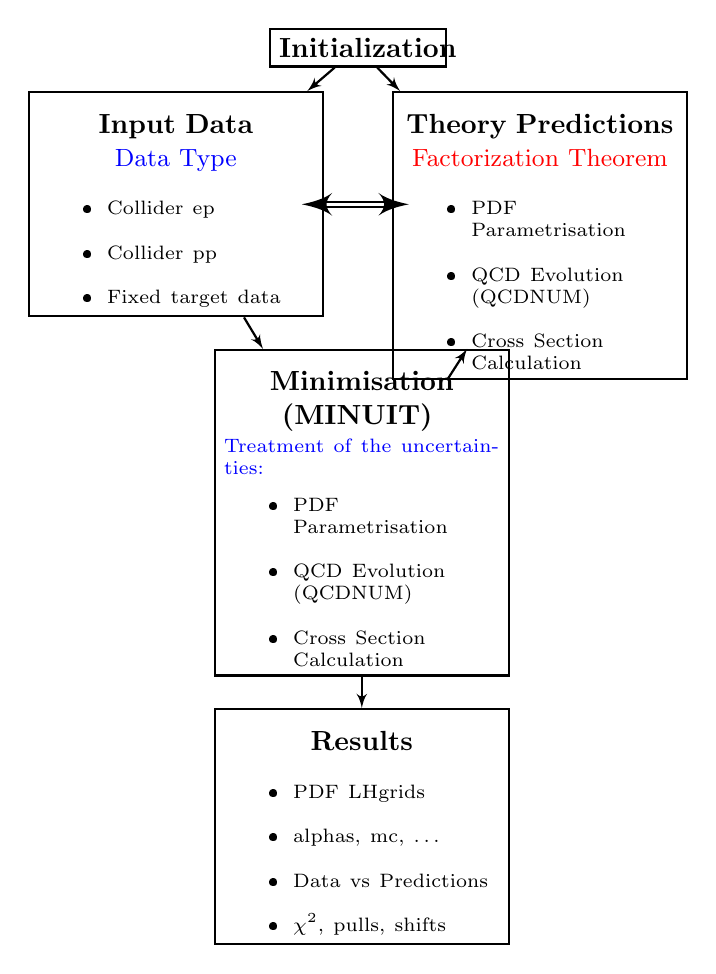
\begin{tikzpicture}[node distance=1cm, auto,>=latex', thick]
      \path[->] node[draw, text width=2cm, align=center] at (0,0) (init) {\bf Initialization};
      \path[->] node[draw, below left=0.3cm and -0.7cm of init, text width=3.5cm] (data) 
                    {\begin{center} \vspace{-0.3cm}{\bf Input Data} 
		      \\ {\color{blue}\small Data Type} 
		     \end{center} 
		     {\scriptsize 
		     \begin{itemize}
                      \vspace{-0.3cm}
		      \item Collider ep
		      \item Collider pp
		      \item Fixed target data
		     \end{itemize}}
		     } (init) edge (data);
      \path[->] node[draw, below right=0.3cm and -0.7cm of init, text width=3.5cm] (theory) 
                    {\begin{center} \vspace{-0.3cm}{\bf Theory Predictions} 
		      \\ {\color{red}\small Factorization Theorem} 
		     \end{center} 
		     {\scriptsize 
		     \begin{itemize}
                      \vspace{-0.3cm}
		      \item PDF Parametrisation
		      \item QCD Evolution (QCDNUM)
		      \item Cross Section Calculation
		     \end{itemize}}
		     } (init) edge (theory);
      \path[->] node[draw, below right=0.4cm and -1.4cm of data, text width=3.5cm] (minuit) 
                    {\begin{center} \vspace{-0.3cm}{\bf Minimisation (MINUIT)} 
                      \vspace{-0.2cm}
		     \end{center} 
		     {\color{blue}\scriptsize Treatment of the uncertainties:} 
		     {\scriptsize 
                      \vspace{-0.1cm}
		     \begin{itemize}
		      \item PDF Parametrisation
		      \item QCD Evolution (QCDNUM)
		      \item Cross Section Calculation
		     \end{itemize}}
		     } (data) edge (minuit)
		     (theory) edge (minuit)
		     (data) ++ (1.6,0) edge [<->,double equal sign distance] ++(1.36,0) (theory);
      \path[->] node[draw, below =0.4cm  of minuit, text width=3.5cm] (res) 
                    {\begin{center} \vspace{-0.3cm}{\bf Results} 
		     \end{center} 
		     {\scriptsize 
		     \begin{itemize}
                      \vspace{-0.3cm}
		      \item PDF LHgrids
		      \item alphas, mc, \dots
		      \item Data vs Predictions
		      \item \(\chi^2\), pulls, shifts
		     \end{itemize}}
		     } (minuit) edge (res);
  \end{tikzpicture}
  \caption{Schematic structure of the \fitter program.} 
  \label{fig:flow}
\end{figure}

%\begin{figure}[!ht]
%   \centering
%   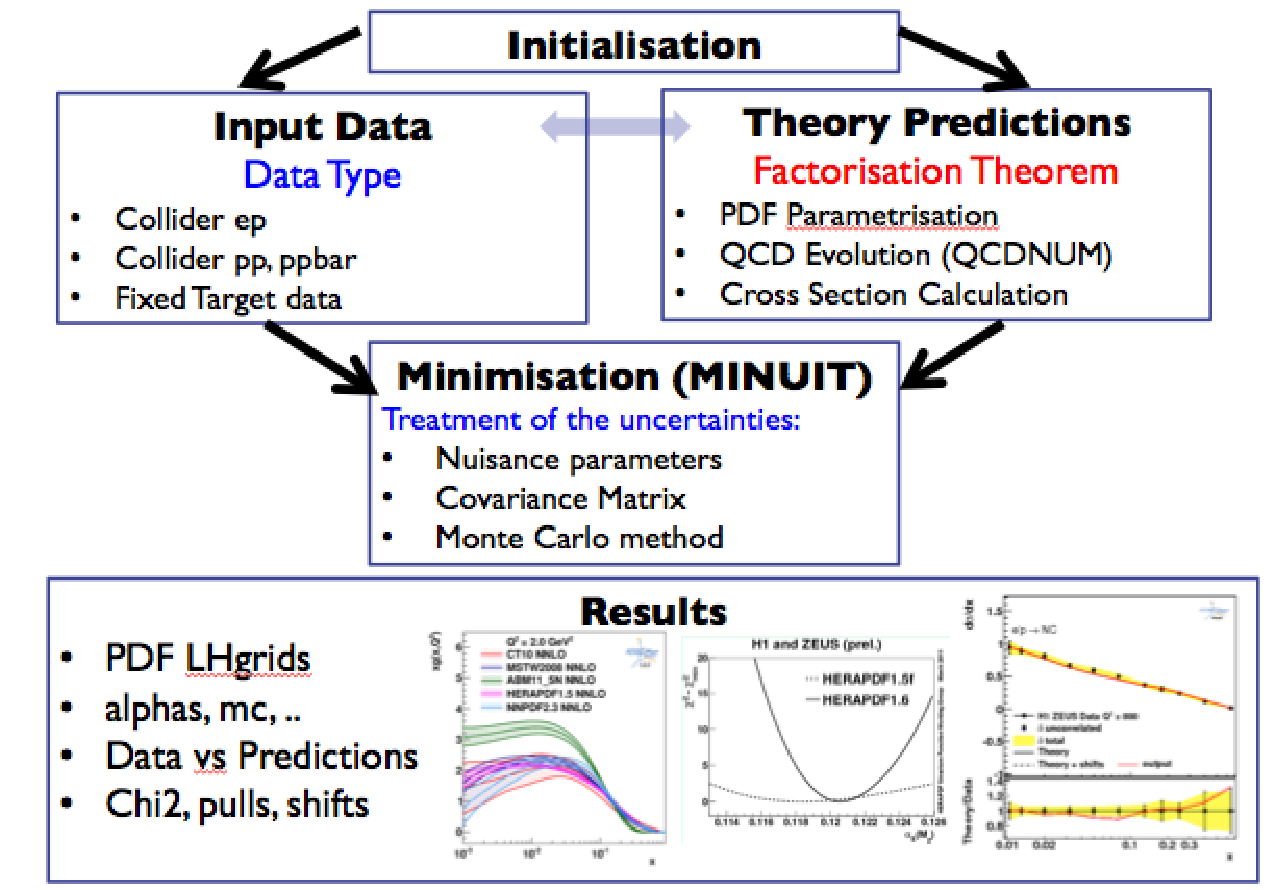
\includegraphics[width=8cm]{flow.pdf}
%   \caption{Schematic structure of the \fitter~program.} 
% \label{fig:flow}
%\end{figure}
\begin{description}
\item 
\bf {Input data:} \rm  All relevant cross section measurements from the various processes
are stored internally in \fitter with the full information on their uncorrelated and correlated
uncertainties. HERA I data sets are the basis of any proton PDF extraction, 
and they are used by all global PDF groups \cite{MSTWpdf, CT10pdf, NNPDFpdf, ABMpdf, JRpdf}. 
Additional measurements provide constraints to the sea flavour decomposition (such as the new 
results from the LHC), as well as constraints to PDFs in the kinematic phase-space regions 
where HERA data is not measured precisely, such as the high $x$ region for the gluon and valence quark distributions.
\item
\bf{Theory predictions:} \rm  Predictions for cross section of different processes are obtained using the factorisation approach (Eq.~\ref{eq:fact}). PDFs are parametrised at a starting scale $Q_0^2$  by a chosen functional form with a set of free parameters $\vec{p}$. These PDFs are then evolved from $Q_0^2$ to the scale of the measurement using the 
Dokshitzer-Gribov-Lipatov-Altarelli-Parisi 
(DGLAP)~\cite{Gribov:1972ri, Gribov:1972rt, Lipatov:1974qm,
Dokshitzer:1977sg, Altarelli:1977zs} evolution equations 
(as implemented in \qcdnum~\cite{qcdnum}), 
CCFM~\cite{\CCFM} or dipole models~\cite{Golec-Biernat:1998js,Iancu:2003ge,Bartels:2002cj} 
and then convoluted with the hard parton cross sections calculated
using a relevant theory program (as listed in Tab.~\ref{tab:proc}).
\item
\bf{PDF fit:} \rm  PDFs are extracted from a least square fit by constructing a 
$\chi^2$ from the input data and the theory prediction.
The $\chi^2$ is  minimized iteratively 
with respect to the PDF parameters using the MINUIT~\cite{minuit} program.
Various choices of accounting for the experimental uncertainties are employed in \fitter, either using 
a nuisance parameter method for the correlated systematic uncertainties, 
or a covariance matrix method (see details in section~\ref{sec:chi2representation}). In addition, \fitter allows to study different statistics 
assumptions for the distributions of the systematic uncertainties (i.e. Gauss or log-normal)~\cite{hera-lhc:report2009}.
%
In the $\chi^2$ minimization,
The parameters $\vec{p}$ of the parametrised PDFs and their uncertainties are extracted from the minimization fit.
%Fitted values of $\vec{p}$ and estimated uncertainties are obtained.
%The fitted parameters $\vec(p)$ and obtained from the uncertainties of the parameters are determined (from chi2+1???)
%
\item
\bf{Results:} \rm 
%The fitted parameters $\vec{p}$ and their estimated uncertainties are produced. 
The resulting PDFs are provided in a format ready to be used by the \lhapdf 
library~\cite{lhapdf,lhapdfweb} or by \tmdlib \cite{tmdlref}.
\fitter drawing tools can be used to display the PDFs with the uncertainty at a chosen scale.  
%Drawing tools are supplied which allow the PDFs to be
%graphically  displayed at chosen scales by the users with their one sigma uncertainty bands. 
A first set of PDFs extracted by \fitter is HERAPDF1.0 \cite{h1zeus:2009wt} (Fig.~\ref{fig:hera1}) 
which is based on HERA~I data.
Since then several other PDF sets were produced within the HERA and LHC collaborations.
In addition to PDF display, 
the figures comparing the data used in the fit and the relevant theory predictions are produced. 
% plots which compare the input data to the fitted theory predictions can be produced 
%to demonstrate the fit consistency. 
\begin{figure}[!ht]
   \centering
   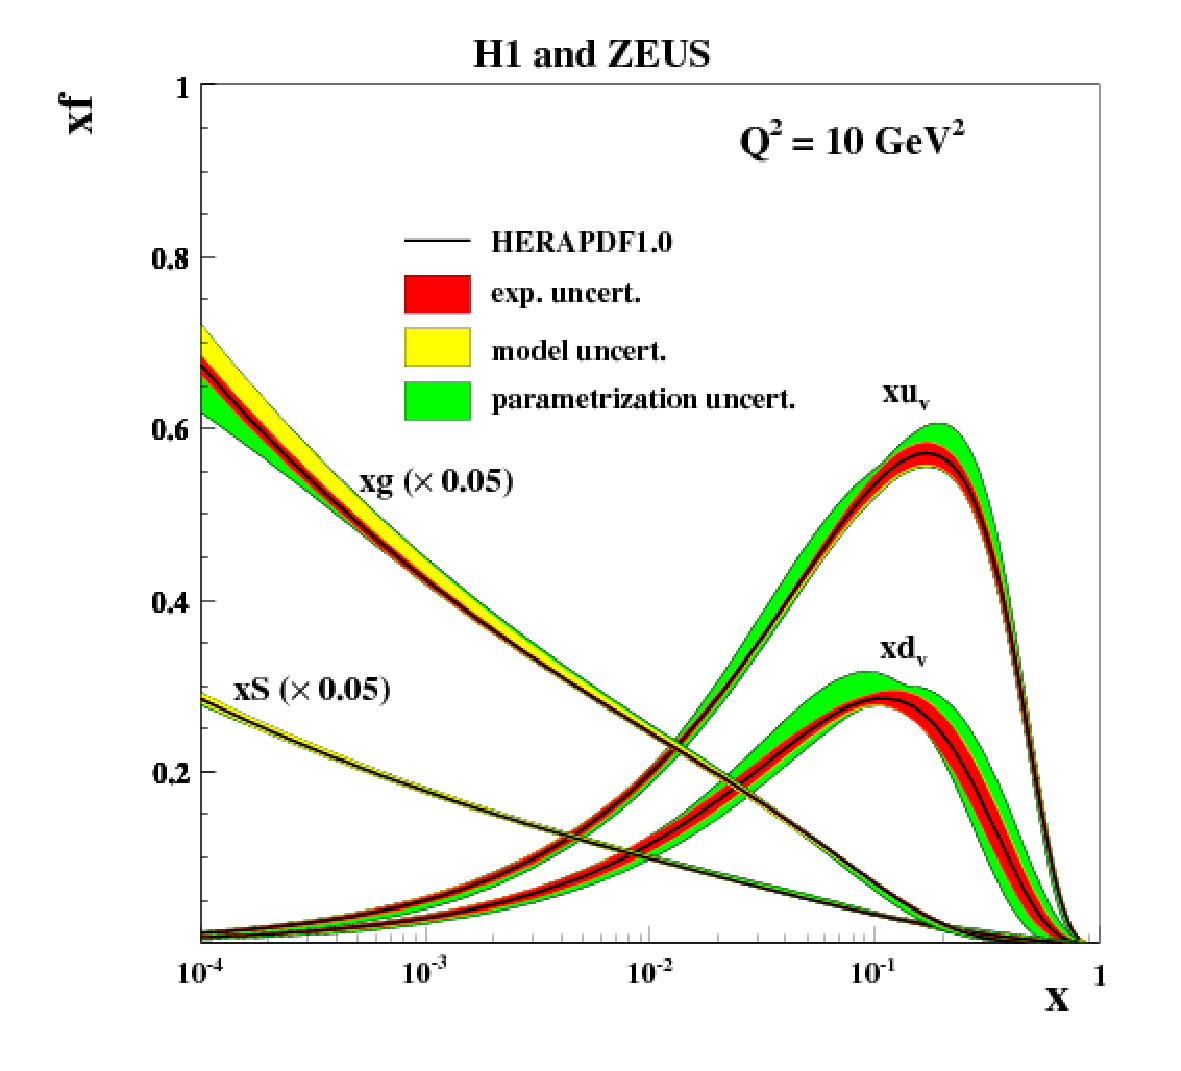
\includegraphics[width=8cm]{hera1.pdf}
   \caption{Summary plots of valence, total sea (scaled) and gluon densities (scaled) with their experimental, model and parametrisation uncertainties at the scale of $Q^2=10 \ \GeV^2$ for the HERAPDF1.0 PDF set at NLO~\cite{h1zeus:2009wt}.}
 \label{fig:hera1}
\end{figure}
In Fig.~\ref{fig:data}, a comparison of inclusive NC data from the HERA~I running period with predictions based on HERAPDF1.0. It also illustrates the comparison to the theory predictions which are adjusted by the  
systematic uncertainty shifts when using the nuisance parameter method that accounts for 
correlated systematic uncertainties. 
As an additional consistency check between data and the theory predictions, pull information, defined as the difference between data and prediction divided by the uncorrelated uncertaintly of the data, is displayed in units of sigma shifts for each given data bin.
% related only to the uncorrelated part of the systematic uncertainty. 

\begin{figure}[!ht]
   \centering
   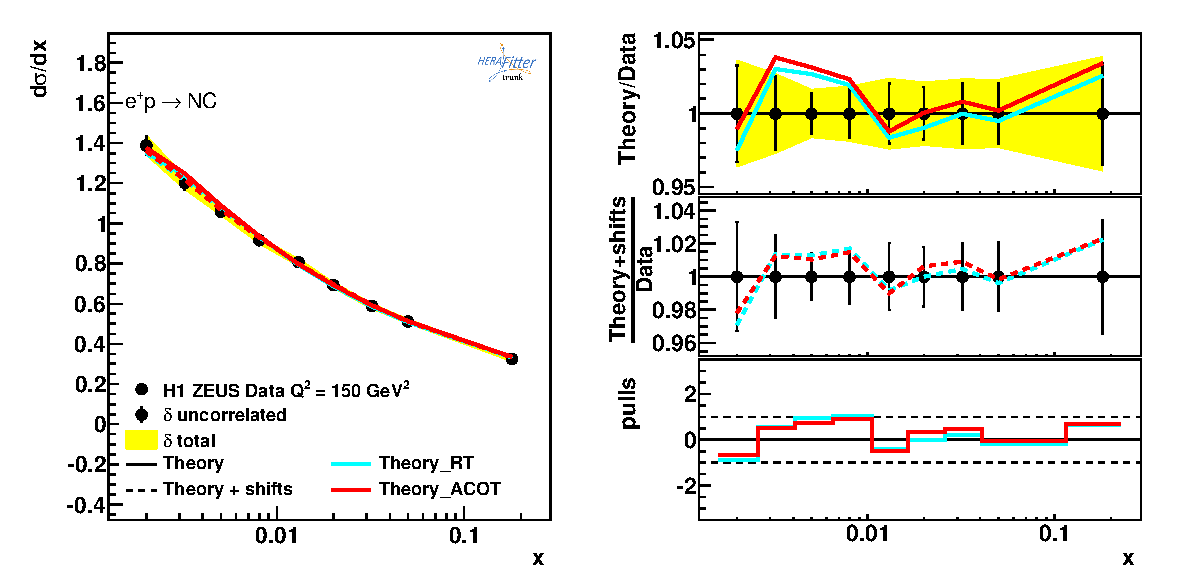
\includegraphics[width=8.6cm]{datatheory.pdf}
   \caption{An illustration of the \fitter drawing tools comparing the measurements (in the case of HERA I) to the predictions of the fit. In addition, ratio plots are also provided together with the pull distribution (right panel).} 
 \label{fig:data}
\end{figure}

\end{description}
%
%This paper provides a comprehensive description of  \\
%the \fitter\ package.
%which is designed for analysis of the High Energy Physics data.
%The package has been developed by members of the H1 and ZEUS collaborations
%with an exclusive support of different theoretical groups.
%The main purpose of the \fitter\ package is analysis of the 
%data from the $e^{\pm}p$, $p\bar{p}$, and $pp$ collider experiments
%information obtained from the deep inelastic scattering experiments
%and the determination of the parton density functions (PDFs).
%The broad range of data taken from the $e^{\pm}p$, $p\bar{p}$, and $pp$ collider experiments can be
%studied by the package. 

%Based on the concept of factorisable nature of the cross sections into universal parton distribution functions (PDFs) and process dependent partonic scattering cross sections, 

%The \fitter\ program facilitates the determination of the PDFs from many 
%cross section measurements at $ep$, $p\bar{p}$ or $pp$ colliders.  
% It includes various options for theoretical calculations and various choices 
%of how to 
%account for the experimental uncertainties. 
The \fitter project provides a versatile environment for benchmarking studies 
and a flexible platform for the QCD interpretation of analyses within the LHC experiments,
as already demonstrated by several publicly available results using the \fitter framework~\cite{atlas:strange,atlas:jets,atlas:hm,cms:strange,cms:jets,h1:2012kk,h1zeus:charm}.  

The outline of this paper is as follows.
%
Section~\ref{sec:theory} discusses the various processes 
and corresponding theoretical calculations performed in the DGLAP~\cite{Gribov:1972ri,Gribov:1972rt,Lipatov:1974qm,
Dokshitzer:1977sg,Altarelli:1977zs} formalism that are available in \fitter.
%
Section~\ref{sec:techniques} presents various techniques employed by the theory calculations used in \fitter.
Section~\ref{sec:method} elucidates the 
methodology of determining PDFs through fits based on various
% {\bf (what do you mean here
%by approaches?)} 
 $\chi^2$ definitions used in the
minimisation procedure. 
Alternative approaches to the DGLAP formalism are presented in section~\ref{sec:alternative}.
%
Specific applications of the package are given in
section~\ref{sec:examples}. 
%
%{\bf add something more here?.}

\section{The HERAFitter Structure}
%
\label{sec:structure}

%\fitter is a flexible open-source platform for the QCD analyses of different experimental measurements, 
%providing a versatile environment for benchmarking studies. It is widely used within the
%LHC experiments~\cite{atlas:strange,atlas:jets,atlas:hm,cms:strange,h1:2012kk,h1zeus:charm}.  

In this section the functionality of \fitter is described.
A block diagram in Fig \ref{fig:flow} gives a schematic view
of the \fitter functionality which can be divided into four main blocks:
\begin{figure}[!ht]
  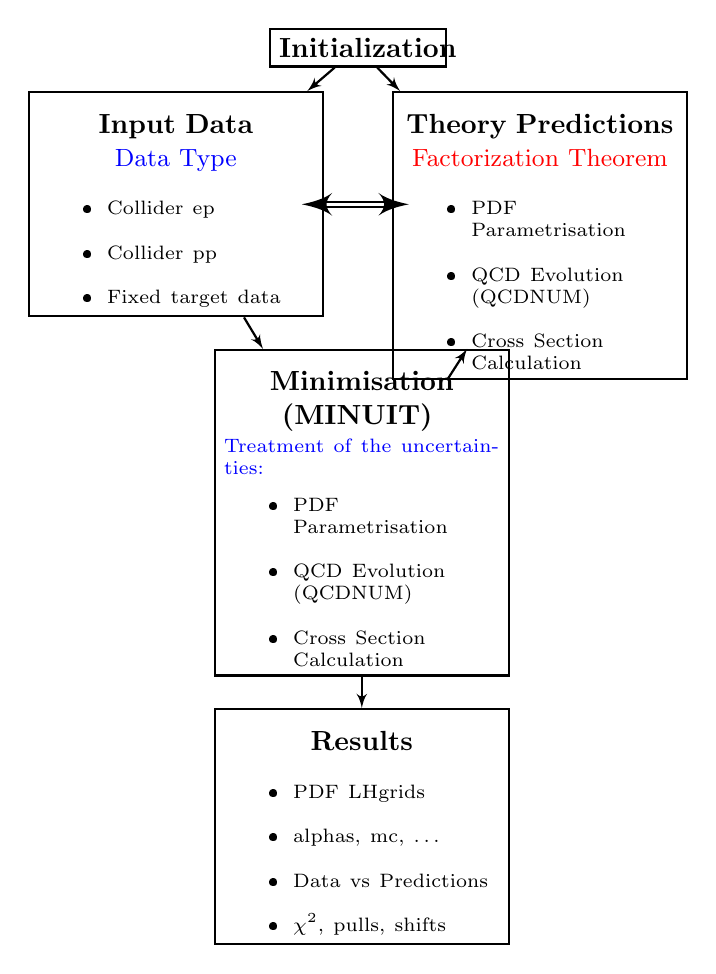
\begin{tikzpicture}[node distance=1cm, auto,>=latex', thick]
      \path[->] node[draw, text width=2cm, align=center] at (0,0) (init) {\bf Initialization};
      \path[->] node[draw, below left=0.3cm and -0.7cm of init, text width=3.5cm] (data) 
                    {\begin{center} \vspace{-0.3cm}{\bf Input Data} 
		      \\ {\color{blue}\small Data Type} 
		     \end{center} 
		     {\scriptsize 
		     \begin{itemize}
                      \vspace{-0.3cm}
		      \item Collider ep
		      \item Collider pp
		      \item Fixed target data
		     \end{itemize}}
		     } (init) edge (data);
      \path[->] node[draw, below right=0.3cm and -0.7cm of init, text width=3.5cm] (theory) 
                    {\begin{center} \vspace{-0.3cm}{\bf Theory Predictions} 
		      \\ {\color{red}\small Factorization Theorem} 
		     \end{center} 
		     {\scriptsize 
		     \begin{itemize}
                      \vspace{-0.3cm}
		      \item PDF Parametrisation
		      \item QCD Evolution (QCDNUM)
		      \item Cross Section Calculation
		     \end{itemize}}
		     } (init) edge (theory);
      \path[->] node[draw, below right=0.4cm and -1.4cm of data, text width=3.5cm] (minuit) 
                    {\begin{center} \vspace{-0.3cm}{\bf Minimisation (MINUIT)} 
                      \vspace{-0.2cm}
		     \end{center} 
		     {\color{blue}\scriptsize Treatment of the uncertainties:} 
		     {\scriptsize 
                      \vspace{-0.1cm}
		     \begin{itemize}
		      \item PDF Parametrisation
		      \item QCD Evolution (QCDNUM)
		      \item Cross Section Calculation
		     \end{itemize}}
		     } (data) edge (minuit)
		     (theory) edge (minuit)
		     (data) ++ (1.6,0) edge [<->,double equal sign distance] ++(1.36,0) (theory);
      \path[->] node[draw, below =0.4cm  of minuit, text width=3.5cm] (res) 
                    {\begin{center} \vspace{-0.3cm}{\bf Results} 
		     \end{center} 
		     {\scriptsize 
		     \begin{itemize}
                      \vspace{-0.3cm}
		      \item PDF LHgrids
		      \item alphas, mc, \dots
		      \item Data vs Predictions
		      \item \(\chi^2\), pulls, shifts
		     \end{itemize}}
		     } (minuit) edge (res);
  \end{tikzpicture}
  \caption{Schematic structure of the \fitter program.} 
  \label{fig:flow}
\end{figure}

%\begin{figure}[!ht]
%   \centering
%   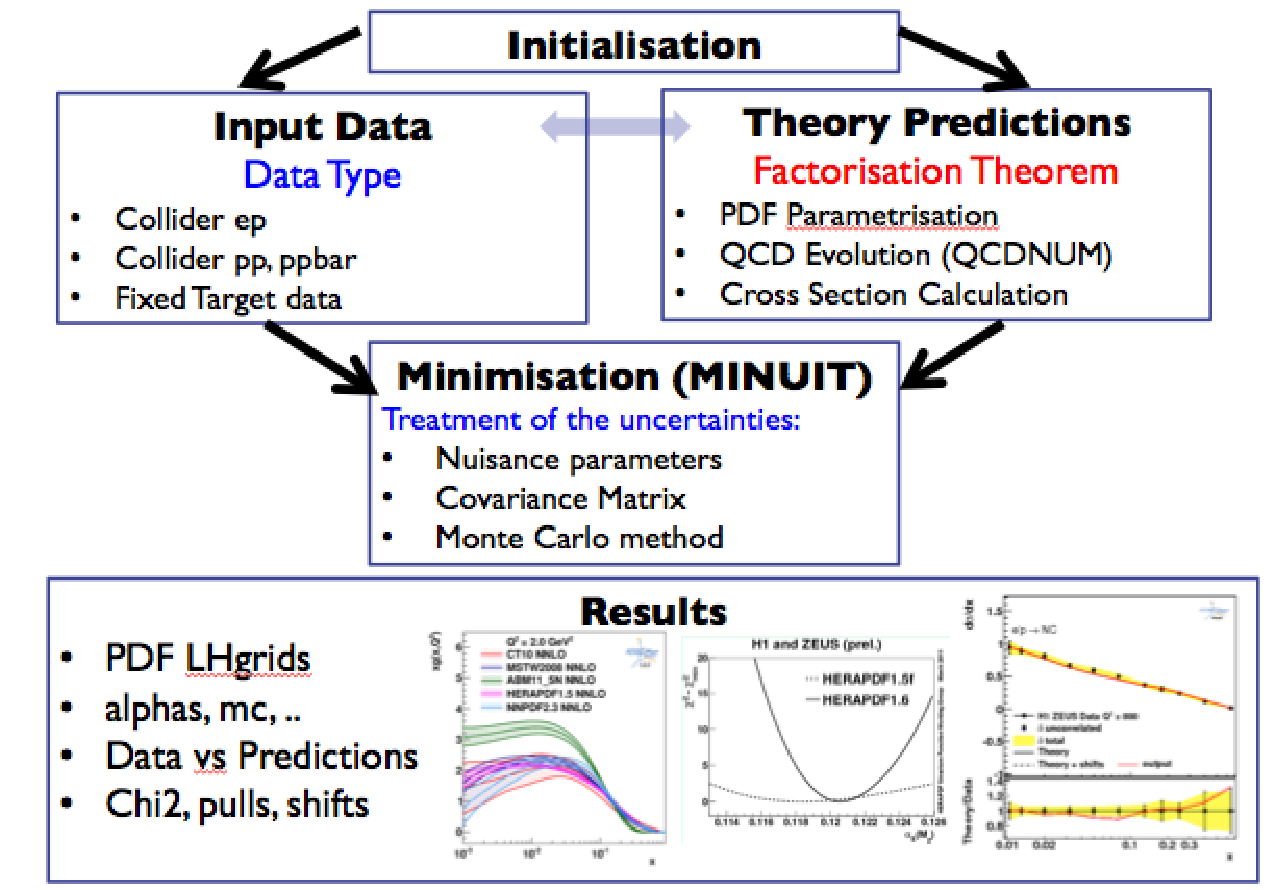
\includegraphics[width=8cm]{flow.pdf}
%   \caption{Schematic structure of the \fitter~program.} 
% \label{fig:flow}
%\end{figure}
%\begin{description}
%\item 
\paragraph{Data:} Different measurements from various processes
are implemented in the \fitter package including the full information on their uncorrelated 
and correlated uncertainties. HERA inclusive scattering data 
are sensitive to quark PDFs and to gluon PDFs through scaling violations and the longitudinal structure function $F_L$.  
%covering low and medium $x$ ranges. 
These data are the backbone of any proton PDF extraction,
and are used by all global PDF groups \cite{MSTWpdf,CT10pdf,NNPDFpdf,Alekhin:2013nda,Jimenez-Delgado:2014twa}.  They can be supplemented by HERA measurements sensitive to heavy quarks and by HERA jet measurements, which have sensitivity to the gluon PDF.
However, the kinematic range of HERA data mostly covers low and medium $x$ ranges.
Improvements in precision of PDFs require additional constraints on the gluon and 
quark distributions at high-$x$, better understanding of heavy quark distributions and 
decomposition of the light-quark sea.  For these purposes, measurements from the fixed-target 
experiments, the Tevatron and the LHC can be used.
% are of particular importance.
%
%Additional measurements provide constraints to the sea flavour decomposition, such as the new 
%results from the LHC, as well as constraints to PDFs in the kinematic phase-space regions 
%where HERA data is not measured precisely, such as the high $x$ region for the gluon and valence 
%quark distributions from Tevatron and fixed target experiments.
%
The processes that are currently available in \fitter framework are listed in Tab.~\ref{tab:proc}.

%
\begin{table}
\small
%\tiny
\scriptsize

\begin{tabular}{|l|l|l|l|}
\hline 
\textbf{Experimental} &\textbf{Process}&\textbf{Reaction}&\textbf{Theory} \\
\textbf{Data}         &        &                &\textbf{calculations, schemes}  \\
\hline \hline \\ [-2.5ex]
%\multirow{6}{*}{HERA} &DIS NC   &$ep\to eX$      & TR', ACOT \\
HERA, &DIS NC   &$ep\to eX$      & TR$^\prime$, ACOT, \\
Fixed Target     &         &                & ZM (\qcdnum), \\
     &         &                & FFN (\texttt{OPENQCDRAD}, \\
     &         &                & \qcdnum), \\ 
     &         &                & TMD (uPDFevolv) \\ [0.5ex]
\hline \\ [-2.5ex]
%\cline{2-4}  \\ [-2.0ex]
HERA &DIS CC   &$ep\to \nu_e X$ & ACOT, ZM (\qcdnum), \\
     &         &                & FFN (\texttt{OPENQCDRAD)} \\  [0.5ex]
\cline{2-4}  \\ [-2.0ex]
     &DIS jets &$ep\to e\ \mathrm{jets}X$      & \nlojetpp (\fastnlo)\\ [0.5ex]
\cline{2-4} \\ [-2.0ex]
     &DIS heavy quarks & $ep\to e c \bar{c} X$, & ZM (\qcdnum), \\
     &         & $ep\to e b \bar{b} X$ & TR$^\prime$, ACOT, \\
     &         &                & FFN (\texttt{OPENQCDRAD}, \\
     &         &                & \qcdnum) \\  [0.5ex]
\hline \\ [-2.5ex]
%Fixed Target   &DIS NC          &$ep\to eX$ & ZM (\qcdnum), \\
%     &         &                & TR', ACOT, \\ [0.5ex]
%     &         &                & FFN (\texttt{OPENQCDRAD}, \\
%     &         &                & \qcdnum) \\  [0.5ex]
%\hline \\ [-2.5ex]
Tevatron,&Drell-Yan &$pp(\bar p)\to l\bar l X$, & \mcfm (\applgrid) \\
LHC              &          &$pp(\bar p)\to l\nu  X$ &                 \\ [0.5ex]
\cline{2-4}  \\ [-2.0ex]
%Tevatron, LHC &W charge asym &$pp(\bar p) \to l\nu X$ & MCFM (\texttt{APPLGRID}) \\
%\hline
              &top pair   &$pp(\bar p) \to t\bar t X$  & \mcfm (\applgrid),  \\
              &            &                            & \texttt{HATHOR}      \\  [0.5ex] 
\cline{2-4}  \\ [-2.0ex]
              &single top &$pp(\bar p) \to t l \nu X$,      & \mcfm (\applgrid) \\
              &           &$pp(\bar p) \to tX$,             &  \\
              &           &$pp(\bar p) \to tWX$             &  \\ [0.5ex]
\cline{2-4}  \\ [-2.0ex]
             &jets &$pp(\bar p) \to \mathrm{jets} X$ & \nlojetpp (\applgrid), \\
                &  & & \nlojetpp (\fastnlo) \\ [0.5ex]
\hline  \\ [-2.5ex] 
LHC& DY+heavy quarks &$pp \to VhX$ & \mcfm (\applgrid) \\  [0.5ex]
\hline
\end{tabular}
\caption{The list of experimental data and theory calculations implemented in the \fitter package. 
The references for the individual calculations and schemes are given in the text.
}
%The APPLGRID~\cite{Carli:2010rw} and FastNLO~\cite{Kluge:2006xs,Wobisch:2011ij,Britzger:2012bs} 
%techniques for the fast interface to theory calculations are described in section~\ref{sec:techniques}.} 
\label{tab:proc}
\end{table}
%
\normalsize
%\item
\paragraph{Theory:}  
%Predictions for cross section of different processes are obtained using 
%the factorisation approach (Eq.~\ref{eq:fact}).
 The PDFs are parametrised at a starting input scale $Q_0^2$  
by a chosen functional form with a set of free parameters $\vec{p}$. 
These PDFs are evolved to the scale of the measurement $Q^2$, $Q^2>Q_0^2$.
The evolution uses the DGLAP formalism \cite{Gribov:1972ri, Gribov:1972rt, Lipatov:1974qm,
Dokshitzer:1977sg, Altarelli:1977zs} (as implemented in \qcdnum~\cite{qcdnum}) by default, however CCFM evolution \cite{\CCFM} is also available 
(as implemented in \texttt{uPDFevolv}~\cite{tmdlref2}).
%or dipole models~\cite{Golec-Biernat:1998js,Iancu:2003ge,Bartels:2002cj}.
The prediction of the cross section for a particular process is obtained, assuming factorisation,  by the convolution of the evolved 
PDFs and the appropriate hard-process parton scattering cross section.
Appropriate theory calculations are listed in Tab.~\ref{tab:proc}.
Alternatively, predictions using dipole models~\cite{Golec-Biernat:1998js,Iancu:2003ge,Bartels:2002cj} can also be obtained.
%\item
\paragraph{QCD Analysis:} \rm  
The PDFs are determined by a least square fit, minimising a $\chi^2$ function, constructed using the input data and theory predictions, with the \minuit \cite{minuit} program.
%with respect to free parameters $\vec{p}$ using the MINUIT~\cite{minuit} program.
%
%extracted from a least square fit by minimising the  $\chi^2$ function with respect to free parameters. 
%The $\chi^2$ function is formed from the input data and the theory prediction.
%The $\chi^2$ is  minimised iteratively 
%with respect to$\vec{p}$ using the MINUIT~\cite{minuit} program.
In \fitter various choices are available to account for the experimental uncertainties. Correlated experimental uncertainties can be accounted for using 
a nuisance parameter method  
or a covariance matrix method as described in section~\ref{sec:chi2representation}.  Different statistical assumptions for the distributions of the systematic uncertainties, like Gaussian or LogNormal~\cite{hera-lhc:report2009} can also be studied (see section~\ref{sec:experimentalerrors}).
%\item
\paragraph{Results:}
%The fitted parameters $\vec{p}$ and their estimated uncertainties are produced. 
The resulting PDFs are provided in a format ready to be used by the \lhapdf 
library~\cite{lhapdf,lhapdfweb} or by \tmdlib \cite{tmdlref}.
\fitter drawing tools can be used to display the PDFs with their uncertainties at a chosen scale.  
%Drawing tools are supplied which allow the PDFs to be
%graphically  displayed at chosen scales by the users with their one sigma uncertainty bands. 
As an example, the first set of PDFs extracted using \fitter from HERA I data, HERAPDF1.0 \cite{h1zeus:2009wt}, 
is shown in Fig.~\ref{fig:hera1} (taken from \cite{h1zeus:2009wt}).
 Note that the PDFs displayed are parton momentum distributions $xf(x,\mu_F^2)$ since this is how PDFs are conventionally stored and displayed.
%%%Since then several other PDF sets were produced within the HERA \cite{hera:grids} and LHC \cite{atlas:grids} collaborations.
%In addition to the PDF display, 
%The comparison of data used in the fit to the theory predictions are also produced. 
% plots which compare the input data to the fitted theory predictions can be produced 
%to demonstrate the fit consistency. 
\begin{figure}[!ht]
   \centering
   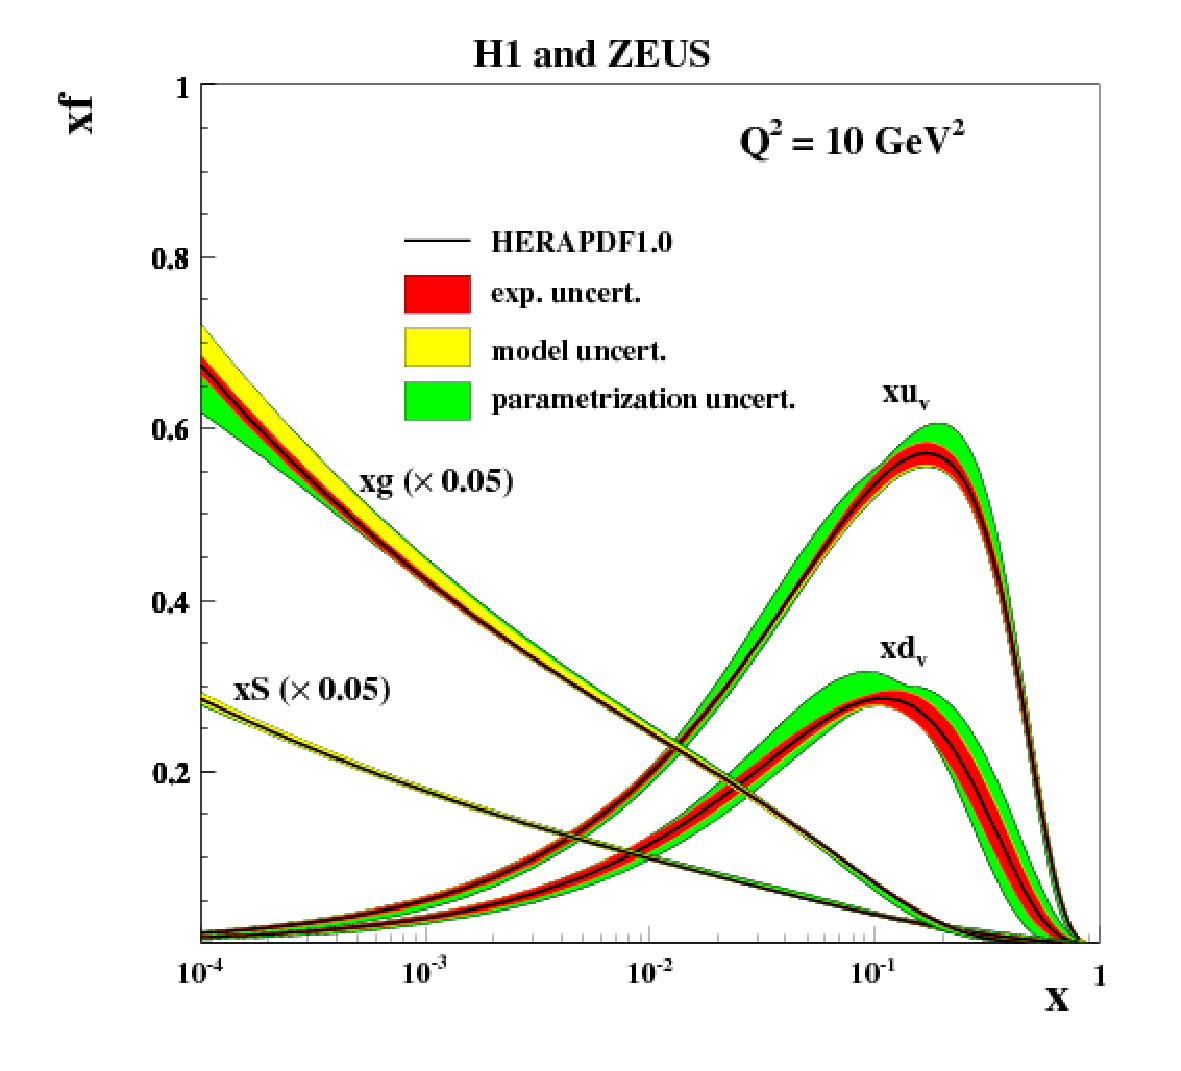
\includegraphics[width=8cm]{hera1.pdf}
   \caption{Distributions of valence ($xu_v$, $xd_v$), sea ($xS$) and the gluon ($g$) densities in HERAPDF1.0~\cite{h1zeus:2009wt}. 
       The gluon and the sea distributions are scaled down by a factor of 20.
       The experimental, model and parametrisation uncertainties are shown as coloured bands.}
       %Summary plots of valence ($xu_v$, $xd_v$), total sea ($xS$, scaled) and gluon ($xg$, scaled) densities
       %with their experimental, model and parametrisation uncertainties shown as colored bands at the scale 
       %of $Q^2=10 \ \GeV^2$ for the HERAPDF1.0 PDF set~\cite{h1zeus:2009wt}.}
 \label{fig:hera1}
\end{figure}
%In Fig.~\ref{fig:data}, a comparison of inclusive NC data from the HERA~I running period with predictions based on HERAPDF1.0 is shown. 
%The inclusive NC data from the HERA I are compared with the predictions based on 
%HERAPDF1.0 PDFs in Fig.~\ref{fig:data}.


%Also shown are theory predictions, obtained using the nuisance parameter method, 
%which accounts for correlated systematic
%shifts when using the nuisance parameter method that accounts for 
%correlated systematic uncertainties (see section~\ref{sec:chi2representation}). 
%The consistency of the measurements and the theory is expressed by pulls, defined as a difference between data 
%and theory divided by the uncorrelated error of the data. 
%In each kinematic bin of the measurement, pulls are provided in units of standard deviation (sigma).  
%As an additional consistency check between data and the theory predictions, pull information, defined as the difference between data and prediction divided by the uncorrelated uncertainty of the data, is displayed in units of sigma shifts for each given data bin.
%\begin{figure}[!ht]
%   \centering
%   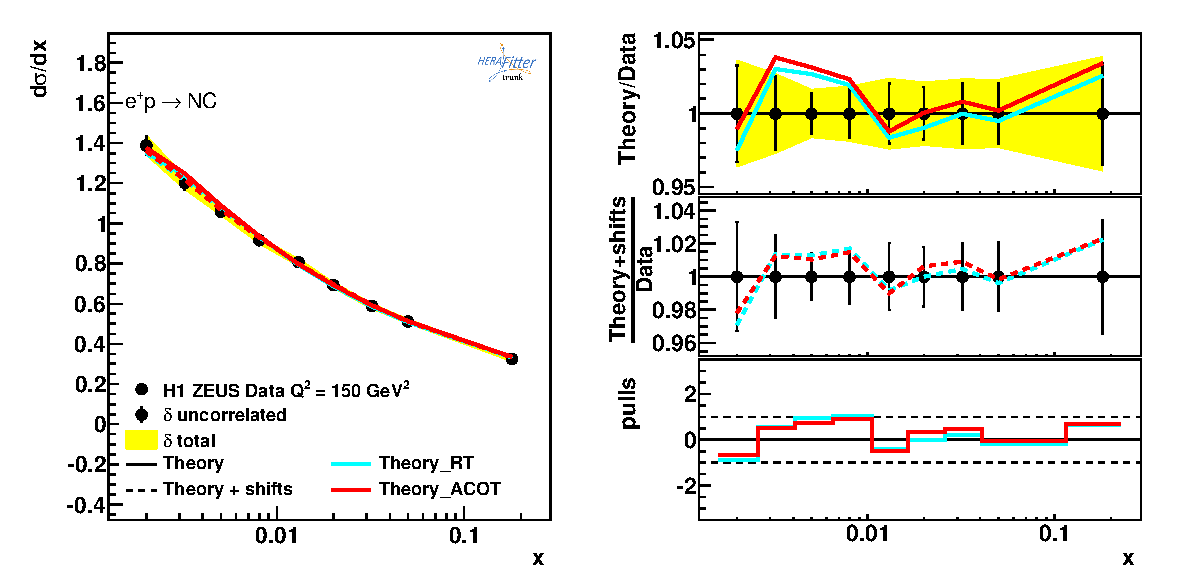
\includegraphics[width=8.6cm]{datatheory.pdf}
%   \caption{An illustration of the consistency of HERA measurements~\cite{h1zeus:2009wt} and the theory predictions, 
%       obtained in \fitter with the default drawing tool.} 
%       %In addition, ratio plots are also provided together with the pull distribution (right panel).}    
% \label{fig:data}
%\end{figure}

%\end{description}
%
%This paper provides a comprehensive description of  \\
%the \fitter\ package.
%which is designed for analysis of the High Energy Physics data.
%The package has been developed by members of the H1 and ZEUS collaborations
%with an exclusive support of different theoretical groups.
%The main purpose of the \fitter\ package is analysis of the 
%data from the $e^{\pm}p$, $p\bar{p}$, and $pp$ collider experiments
%information obtained from the deep inelastic scattering experiments
%and the determination of the parton density functions (PDFs).
%The broad range of data taken from the $e^{\pm}p$, $p\bar{p}$, and $pp$ collider experiments can be
%studied by the package. 

%Based on the concept of factorisable nature of the cross sections into universal parton distribution functions (PDFs) and process dependent partonic scattering cross sections, 

%The \fitter\ program facilitates the determination of the PDFs from many 
%cross section measurements at $ep$, $p\bar{p}$ or $pp$ colliders.  
% It includes various options for theoretical calculations and various choices 
%of how to 
%account for the experimental uncertainties. 
%The \fitter project provides a versatile environment for benchmarking studies 
%and a flexible platform for the QCD interpretation of analyses within the LHC experiments,
%as already demonstrated by several publicly available results using the \fitter 
%framework~\cite{atlas:strange,atlas:jets,atlas:hm,cms:strange,cms:jets,h1:2012kk,h1zeus:charm}.  

\section{Theoretical formalism using DGLAP evolution}
\label{sec:theory}


%The proton PDFs are classically extracted from QCD fits by a measure of 
%the agreement between experimental data and corresponding theory models.
%During the fit procedure in the \fitter\ framework, the PDFs are
%parametrised at a starting scale $Q^2_0$ chosen to be below the charm 
%mass threshold and then evolved using coupled, integro-differential
%Dokshitzer-Gribov-Lipatov-Altarelli-Parisi 
%(DGLAP)~\cite{Gribov:1972ri,Gribov:1972rt,Lipatov:1974qm,
%Dokshitzer:1977sg,Altarelli:1977zs} evolution equations 
%as implemented in the QCDNUM~\cite{qcdnum} program in the $\overline{\text{MS}}$ scheme. 
%The evolution can be performed in the LO, NLO or NNLO accuracy~\cite{Curci:1980uw,Furmanski:1980cm}.
%
In this section the theoretical formalism based on DGLAP evolution equations for various processes 
available in \fitter is described. 

A direct consequence of factorisation (Eq. \ref{eq:fact}) is that scale dependence or ``evolution'' of PDFs can be predicted 
by the renormalisation group equations. 
By imposing that physical observables are independent on 
$\muf$, it leads to a representation 
of parton evolution in terms of 
DGLAP \cite{Gribov:1972ri,Gribov:1972rt,Lipatov:1974qm,Dokshitzer:1977sg,Altarelli:1977zs} equations:
%integro-differential equations known as 
%DGLAP~\cite{Gribov:1972ri,Gribov:1972rt,Lipatov:1974qm,Dokshitzer:1977sg,Altarelli:1977zs} (Dokshitzer-Gribov-Lipatov-Altarelli-Parisi) equations:

\begin{small}
\begin{eqnarray}
\frac{d~f_i(x,\mur,\muf)}{d \log\muf^2} = \sum_{j=q\bar{q},g}\int_{x}^{1}\frac{d y}{y} 
P_{ij}\left(\frac{x}{y};\alpha_s,\mur,\muf\right) f_j(y,\mur,\muf)\,,
\label{eq:dglap}
\end{eqnarray}
\end{small}

where the functions $P_{ij}$ are the evolution kernels or splitting functions, which represent the probability 
of finding parton $i$ in parton $j$, and have perturbative expansion in $\alpha_s$. 
The analytic structure of $P_{ij}$ is known at 3-loop in perturbation theory and can be found in the literature. 

Once PDFs are determined by a direct comparison with the experiments at the initial
scale $Q_0$, their evolution at the scale $\mu$ is entirely determined by DGLAP equations.
Alternative approaches to DGLAP evolution, valid in different kinematic regimes, are also implemented in \fitter and will be discussed in the next sections.


%The PDFs are determined by measuring the agreement 
%the agreement between experimental data and corresponding theory models within 
%the DGLAP~\cite{Gribov:1972ri,Gribov:1972rt,Lipatov:1974qm,
%Dokshitzer:1977sg,Altarelli:1977zs} formalism.
%Models which are available in \fitter\ for various processes are described in the following text.



\subsection{Deep Inelastic Scattering and Proton Structure}
\label{dissection}


DIS data provide the backbone of any PDF fit.
The for\-ma\-lism that relates the DIS measurements to pQCD and the PDFs has been described
in detail in many extensive reviews (see e.g.~\cite{disbook}) and it is only briefly summarised here.
DIS is the process where a lepton scatters off the constituents of the proton
by a virtual exchange of a NC 
or CC vector boson and, as a result, a scattered lepton and a 
multi-hadronic final state are produced.
The common DIS kinematic variables are the absolute squared four-momentum of 
the exchange boson, $Q^2$, the Bjorken $x$, 
%which can be related in the parton model to 
%the fraction of momentum carried by the struck quark, 
and the inelasticity $y$, related by $y=Q^2/sx$, where $s$ is the squared centre-of-mass (c.o.m.) energy.
%$s = 4E_eE_p$ at HERA.
%which is the fraction of the energy 
%transferred to the hadronic vertex.
\\
%
The NC cross section can be expressed in terms of generalised structure functions:
\begin{eqnarray}
%  \nonumber
   \frac{d^2\sigma_{NC}^{e^{\pm} p}}{dxdQ^2}&=&\frac{2\pi\alpha^2}{xQ^4}\cdot \sigma_{r,NC}^{e^{\pm} p},\\ 
   \sigma_{r,NC}^{e^{\pm} p}&= &  Y_{+} \tilde F_2^{\pm} \mp Y_{-}x \tilde F_3^{\pm} - y^2 \tilde F_L^{\pm},
 %\label{eq:NC not reduced}
\end{eqnarray}
where the electromagnetic coupling constant $\alpha$, the photon propagator and a helicity factor are absorbed in the definition of reduced cross section $\sigma_r$, and  $Y_{\pm} = 1 \pm (1-y)^2$ (additional terms of $O(1/Q^2)$ are numerically small 
at the HERA kinematics and are neglected). 
The generalised structure functions $\tilde F_{2,3}$ 
can be written as linear combinations of the proton structure functions $F_2^{\gamma}, F_{2,3}^{\gamma Z}$ 
and $F_{2,3}^Z$ associated to pure photon exchange terms, photon-$Z$ interference
terms and pure $Z$ exchange terms, respectively. 
The structure function $\tilde F_2$ is the dominant contribution to the cross section, 
$x \tilde F_3$ becomes important at high $Q^2$ and $\tilde F_L$ is sizable 
only at high $y$. 
%In the framework of pQCD the structure functions are directly related to the 
%PDFs, i.e. in leading order (LO)  $F_2$ is the weighted momentum sum of quark and anti-quark distributions, 
%$F_2 \approx x \sum e^2_q (q+ \overline q)$, $xF_3$ is related to their difference, 
%$xF_3 \approx x \sum 2e_q a_q (q- \overline q)$ (where $a_q$ is the axial-vector 
%quark coupling and $e_q$ the quark electric charge) and $F_L$ vanishes. 
%At higher orders, terms related to the gluon density distribution
%($\as g$) appear, in particular $F_L$ is strongly related to the low-$x$ 
%gluon.
\\
The inclusive CC $ep$ cross section, analogous to the NC case, can be expressed in terms of another set 
of structure functions and in LO in $\alpha_s$, the $e^+p$ and $e^-p$ cross sections are sensitive to 
different combinations of the quark flavour densities:
\begin{eqnarray}
\centering
%  \nonumber
%    \begin{array}{rll}
   \frac{d^2\sigma_{CC}^{e^{\pm} p}}{dxdQ^2}&=&\frac{1\pm P}{2}\frac{G^2_F}{2\pi x}\big [\frac{M^2_W}{M^2_W+Q^2}\big ]\cdot \sigma_{r,CC}^{e^{\pm} p}\\
   \sigma_{r,CC}^{e^{\pm} p}&= &  Y_{+} \tilde W_2^{\pm} \mp Y_{-}x \tilde W_3^{\pm} - y^2 \tilde W_L^{\pm},
%      \sigma_{r,CC}^{e^{+} p} &\approx& 
%        x [\overline u + \overline c] + (1-y)^2 x [d+s], \\
%      \sigma_{r,CC}^{e^{-} p} &\approx& 
%        x[u+c] + (1-y)^2 x[\overline d + \overline s],
%    \end{array}
\end{eqnarray}
where $P$ represents the lepton beam polarisation and $\tilde W_2$, $\tilde W_3$,$\tilde W_L$ are structure functions.
%Here $U$ and $D$ denote the sum over up- and down-type quarks;
%the latter include also strange and beauty quarks and 
%the former charm quarks.
%
%Beyond LO, 
%{\bf check this sentence if it makes sense}.
The QCD predictions for the DIS structure functions are obtained by convoluting 
the PDFs with the respective coefficient functions. 

The DIS measurements
span a large range of $Q^2$ from few GeV$^2$ to about $10^5$ GeV$^2$,
%from low to high $Q^2$
crossing heavy-quark mass thresholds, thus the
treatment of heavy quarks (charm and beauty) and of their masses becomes important. 
There are different approaches to the treatment of heavy quark production that should 
be equivalent if calculations are carried out to all orders in $\alpha_s$. 
Several variants of these schemes are implemented in \fitter and they are briefly discussed below.


%\begin{description}
\paragraph{Zero-Mass Variable Flavour Number (ZM-VFN)\cite{ZMVFNpub}:}

In this scheme, the
heavy quark densities appear in the proton at $Q^2$ values above $\sim m_h^2$ (heavy quark mass)
and the heavy quarks
%for $Q^2>>m_h^2$ but 
are treated as massless in both the initial 
and final states of the hard scattering process. The lowest order process is the
%scattering of a heavy quark in the proton with the lepton via (electroweak) boson exchange.
scattering of lepton off the heavy quark via boson exchange.
This scheme is expected to be reliable only in the region with $Q^2 \gg m_h^2$.
%This is the scheme that had been used in the past by PDF groups.
In \fitter this scheme is available for the DIS structure function calculation 
via the interface to the \qcdnum \cite{qcdnum} package and it benefits 
from the fast \qcdnum convolution engine.

\paragraph{Fixed Flavour Number (FFN)\rm \cite{Laenen:1992, Laenen:1993, Riem:1995}:} 

In this scheme only the gluon and the light quarks are considered
as partons within the proton and massive 
quarks are produced perturbatively in the final state.
The lowest order process is
the heavy quark-antiquark pair production in the boson-gluon fusion.
%the fusion of a gluon in the proton
%with a boson from the lepton to produce a heavy quark and an antiquark.
%The recent series of PDFs that use this scheme as default are ABM and JR PDF groups.
In \fitter this scheme can be accessed via the 
\qcdnum implementation or through the interface to the open-source code \texttt{OPENQCDRAD}~\cite{openqcdrad:page}, as implemented by the ABM group.
Through \qcdnum, the calculation of the heavy quark contributions to DIS structure functions
are available at Next-to-Leading-Order (NLO), at $O(\as^2)$, and only electromagnetic exchange contributions are taken into account.
Through the ABM implementation the heavy quark contributions to CC structure functions are available 
%and, for the NC case, the QCD corrections to the massive Wilson coefficients at Next-to-Next-to Leading Order (NNLO)
and, for the NC case, the QCD corrections to the coefficient functions at Next-to-Next-to Leading Order (NNLO)
are provided at the best currently known approximation~\cite{SMoch:npb864}.
The ABM implementation also includes 
the definition in $\overline{\text{MS}}$ scheme with the running heavy-quark mass \cite{Alekhin:runm}.
The scheme has the advantage of reducing the sensitivity of the DIS cross sections to
higher order corrections, and improving the theoretical precision of the mass definition. 


\paragraph{General-Mass Variable Flavour Number (GM-VFN)\rm \cite{VFN}:}

It this scheme, heavy quark production is treated for
$Q^2 \le m_h^2$ in the FFN scheme and for $Q^2 \gg m_h^2$
in a massless scheme. 
%in the ZM-VFN scheme with a suitable interpolation in between.
The recent series of PDF groups that use this scheme are MSTW, CT(CTEQ), NNPDF, and HERAPDF.
%This scheme is very popular and numerous variants exist.
\fitter implements different variants of the GM-VFN scheme and they are presented below:
% 
\begin{itemize}
%
\item \it {GM-VFN Thorne-Roberts scheme:} \rm
%\subsubsection{GM-VFN Thorne-Roberts scheme}
%
%The Thorne-Roberts (TR) scheme provides a smooth transition from the massive FFN
%scheme at low scales $Q^2<m_h^2$ to the massless ZM-VFNS scheme at  
%high scales $Q^2>>m_h^2$.
%There are two different variants of the TR schemes: TR standard 
%(as used in MSTW PDF 
%sets~\cite{Thorne:1997ga,Thorne:2006qt,MSTWpdf}) 
%and TR optimal~\cite{Thorne:6180}, with a smoother transition across the heavy quark threshold region.
%Both of these variants are accessible within the \fitter package at 
%NLO and NNLO.  
%
The Thorne-Roberts (TR) scheme~\cite{Thorne:1997ga} was designed to provide a smooth transition 
from the massive FFN scheme at low scales $Q^2 < m_h^2$ to the massless ZM-VFNS scheme at high scales $Q^2 \gg m_h^2$. 
However, the original version was technically difficult to implement beyond NLO, and was updated 
to the TR$^\prime$ scheme~\cite{Thorne:2006qt}.
%which is simpler (and closer to the ACOT-scheme, see below).
There are two different variants of the TR$^\prime$ schemes: TR$^\prime$ standard (as used in MSTW PDF sets~\cite{Thorne:2006qt,MSTWpdf}) 
and TR$^\prime$ optimal~\cite{Thorne:6180}, with a smoother transition across the heavy quark threshold region. 
Both variants are accessible within the \fitter package at LO, NLO and NNLO.
%%%%
\vspace{0.1cm}
\item \it {GM-VFN ACOT scheme:} \rm
The Aivazis-Collins-Olness-Tung (ACOT) scheme belongs to the group of VFN factorisation 
schemes that use the renormalisation method of Collins-Wilczek-Zee (CWZ) \cite{CWZ}.
This scheme unifies the low scale $Q^2 < m_h^2$ and high scale $Q^2 > m_h^2$ regions with a smooth interpolation across the full energy range. 
%It is built upon the massive factorisation theorem by Collins~\cite{CWZ} 
%to incorporate the heavy quark masses for $Q^2 > m_h^2$; hence, it can be consistently applied 
%order by order in the perturbation theory.
%
%This scheme involves a mixture of the $\overline{\text{MS}}$ scheme 
%for light and heavy (when the factorisation scale is larger than the heavy quark mass) partons
%and the zero-momentum subtraction renormalisation scheme for graphs with heavy quark lines 
%(if the factorisation scale is smaller than the mass of the heavy quark threshold). 
%% is this sentence below is important?
%%The DGLAP kernels and PDF evolution are pure $\overline{\text{MS}}$, 
%%therefore, the ACOT scheme is considered to be a minimal extension of the $\overline{\text{MS}}$ scheme.
Within the \tt ACOT\rm package, different variants of the ACOT scheme are available:
ACOT-Full \cite{Aivazis:1993pi}, S-ACOT-$\chi$ \cite{Kramer:2000hn,Kretzer:2003it}, ACOT-ZM \cite{Aivazis:1993pi}, 
$\overline{\text{MS}}$ at LO and NLO. 
For the longitudinal structure function higher order calculations are also available. 
%The ACOT-Full implementation takes into account the quark masses 
%and it reduces to ZM $\overline{\text{MS}}$ scheme in the limit of masses going to zero, 
%but it has the disadvantage that it is computationally intensive (addressed in 
%section~\ref{sec:techniques}).
A comparison of PDFs extracted from the QCD fits to the HERA data 
with the TR$^\prime$ and ACOT-Full schemes is illustrated in Fig.~\ref{fig:acotrt} as taken from \cite{h1zeus:2009wt}.

\begin{figure}[!ht]
\centering
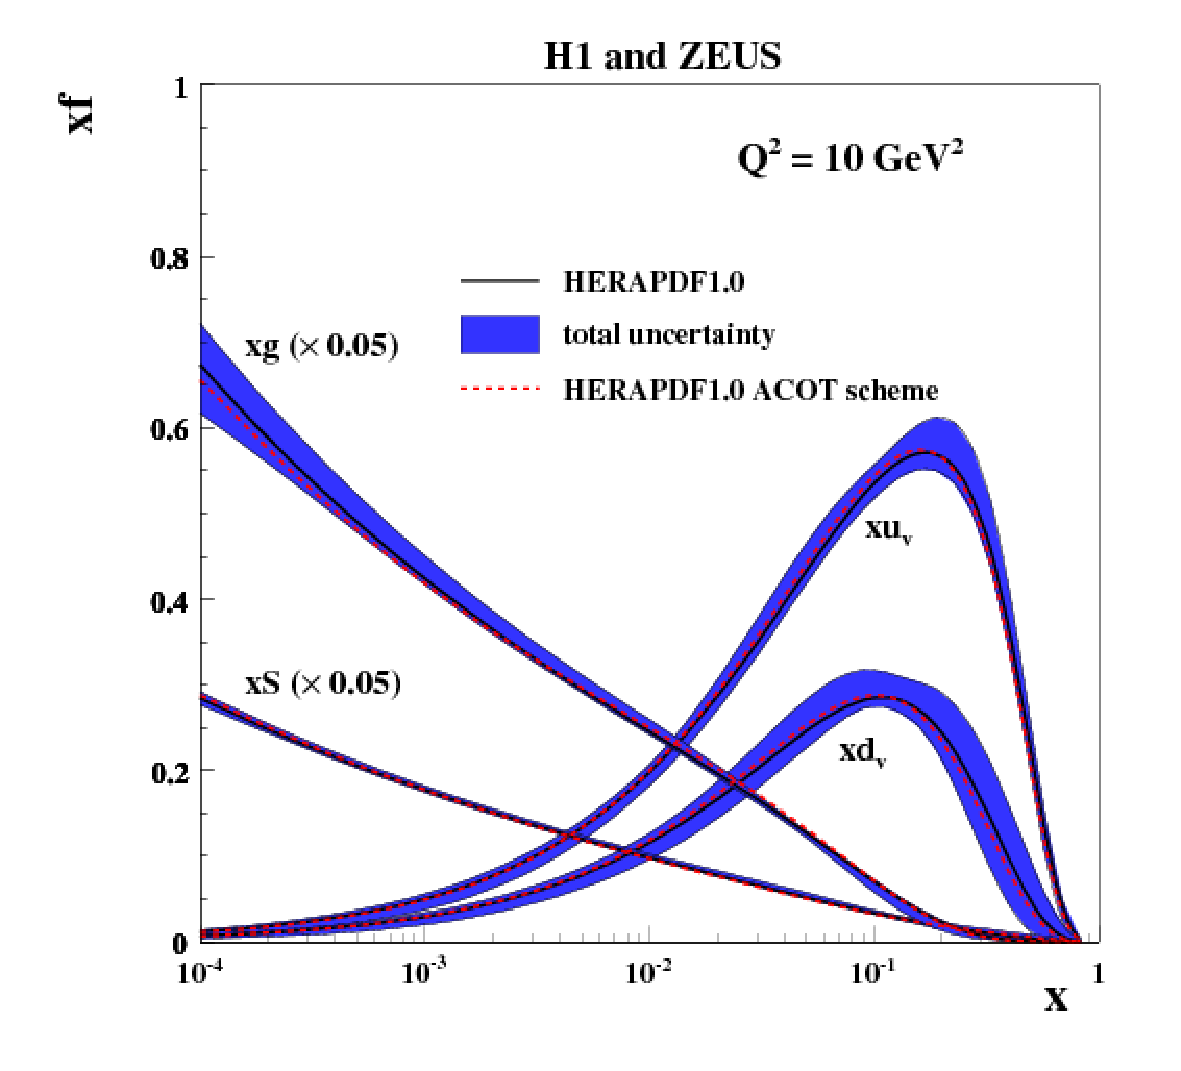
\includegraphics[width=8cm]{heraacot}
  \caption{Overview showing the $u$- and $d$-valence, the total sea
    (scaled), and gluon (scaled) PDFs of the NLO HERAPDF1.0 set \cite{h1zeus:2009wt} 
    with their 
    total uncertainty at the scale of $Q^2 = 10\ \GeV^2$ obtained 
    using the TR$^\prime$ scheme and compared to the PDFs obtained with 
    the ACOT scheme using the $k$-factor technique (red).}
 \label{fig:acotrt}
\end{figure}


%\vspace{0.1cm}
\end{itemize}
%\end{description}

\subsection{Electroweak Corrections to DIS}
%%%%%%%%%%%
%\item \bf {Electroweak corrections for \texorpdfstring{$ep$}{ep} scattering:} \rm
Calculations of higher-order electroweak corrections to DIS scattering at 
HERA are available in \fitter in the on-shell scheme. In this scheme the
gauge bosons masses $M_W$ and 
$M_Z$ are treated symmetrically as basic parameters together with the top, 
Higgs and fermion masses.
These electroweak corrections 
are based on the \tt EPRC\rm package~\cite{SpiesbergerPrivComm}.
The code provides the running of electromagnetic coupling $\alpha$ using the most recent parametrisation
of the hadronic contribution to $\Delta_\alpha$ \cite{Jegerlehner}, as well as 
an older version from Burkhard \cite{Burkhard}.



\subsection{Diffractive PDFs}

\newcommand{\asotp}{\ensuremath{\frac{\alpha_{\rm s}}{2\pi}}}
\newcommand{\Sgl}[1]{\ensuremath{\tilde f_{#1+}}}
\newcommand{\Pom}{{I\!P}}
\newcommand{\Reg}{{I\!R}}
\newcommand{\xpom}{$x_{I\!P}$}
\newcommand{\xP}{x_\Pom}


Similarly to standard PDFs, diffractive parton distributions (DPDFs) 
can be determined from QCD fits to diffractive cross sections.
%In this section the diffractive process is briefly described.
About 10\% of deep inelastic interactions at HERA are diffractive, i.e. leading to
events in which the interacting proton stays intact ($ep\to eXp$). 
In the diffractive process the proton is well separated from the 
rest of the hadronic final state by a large rapidity gap.  
This is interpreted as the dissociation of the virtual photon into
hadronic system $X$ with the invariant mass much 
smaller than the photon-proton c.o.m. energy $W=ys-Q^2+m_p^2(1-y)$, where $m_p$ is proton's mass,  and the same net 
quantum numbers as the exchanged photon.
%Figure~\ref{fig:diff} illustrates the kinematic variables used to describe
%the inclusive diffractive DIS process. 
For such a processes, the 
%proton vertex factorisation approach
%is assumed where 
diffractive DIS is mediated by the exchange of a hard Pomeron 
or a secondary Reggeon with the vacuum quantum numbers. 
The factorisable pomeron picture has proved remarkably successful in the description of most of these data.
%
%\begin{figure}[!ht]
%\begin{center}
%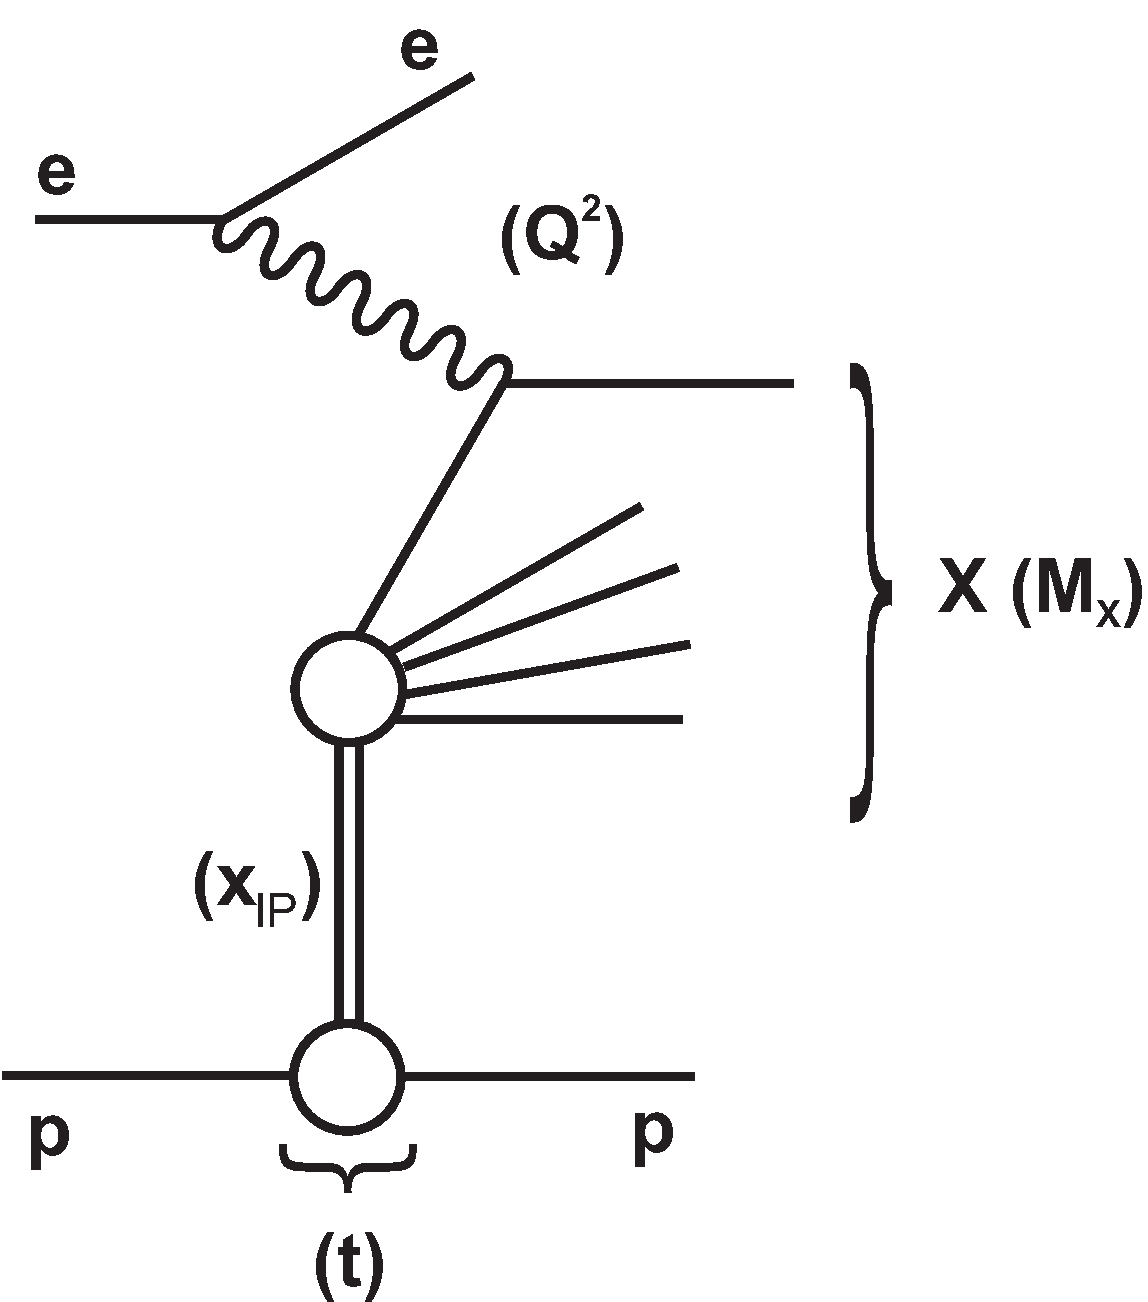
\includegraphics[width=0.5\linewidth]{figures/diffraction.pdf}
%\end{center}
%\caption{Schematic diagram of the kinematic variables used to
% describe the inclusive diffractive DIS process.}
%\label{fig:diff}
%\end{figure}

The kinematic variables squared four-momentum transfer $t$
(the undetected momentum transfer to the proton system) and
the mass $M_X$ of the diffractively produced final state 
appear for the diffractive process in addition to the usual DIS variables $x$, $Q^2$.
In practice, the variable $M_X$ 
is often replaced by dimensionless quantity $\beta=\frac{Q^2}{M_X^2+Q^2-t}$.
%
In models based on a factorisable pomeron, $\beta$ may be viewed at LO as the fraction of the
pomeron longitudinal momentum which is carried by the struck parton, $x=\beta x_{\Pom}$.
%The diffractive parton distribution functions (DPDFs) are interpreted as probabilities for 
%finding a parton with a small fraction of the proton momentum $x=\beta\Pom$
\\
For the inclusive case, the diffractive cross-section reads as:
\begin{equation}
\begin{array}{lcl}
  \frac{d\sigma}{d\beta\,dQ^2dx_{\Pom}\,dt}
=
  \frac{2\pi\alpha^2}{\beta Q^4}\,
    \left( 1 +  (1-y)^2 \right) \ensuremath{\overline\sigma}^{D(4)}(\beta,Q^2,x_{\Pom},t)
\label{Dxs}
\end{array}
\end{equation}
with the ``reduced cross-section'': 
\begin{equation}
\begin{array}{lcl}
\overline\sigma^{D(4)}
 = F_2^{D(4)} - \frac{y^2}{1 +  (1-y)^2}\, F_L^{D(4)}.
% = F_T^{D(4)} + \frac{2(1-y)}{1 +  (1-y)^2}\, F_L^{D(4)}.
\label{eq:sigred}
\end{array}
\end{equation}
%The dimension of $F_k^{D(4)}(\beta,Q^2,x_{\Pom},t)$
%is $GeV^{-2}$ and thus quantities integrated over $t$.
%\begin{equation}
%F_k^{D(3)}(\beta,Q^2,x_{\Pom})
%\equiv
%\int_{t_{\rm min}}^{t_{\rm max}} dt
%F_k^{D(4)}(\beta,Q^2,x_{\Pom},t)
%\end{equation}
%are dimensionless. The maximum kinematically allowed value of $t$ is given by
%\begin{equation}
%t_{\rm MAX} 
%=
%-\frac{x_{\Pom}^2 m_p^2 + p_\perp^2}{1-x_{\Pom}}
%\approx 
%-\frac{x_{\Pom}^2}{1-x_{\Pom}} m_p^2
%\end{equation}
%where $m_p$ is the proton mass.
Substituting $x = x_{\Pom}\beta$ we can relate Eq.~\ref{Dxs} to the standard DIS formula.
%\begin{equation}
%\begin{array}{lcl}
%\frac{d\sigma}{d\beta\,dQ^2\,dx_{\Pom}\,dt} =
%  \frac{2\pi\alpha^2}{x\, Q^4}\,
%    \left( 1 +  (1-y)^2 \right) x_{\Pom}\ensuremath{\overline\sigma}^{D(4)}(\beta,Q^2,x_{\Pom},t)
%\end{array}
%\end{equation}
%which upon integration over $t$ reads
%\begin{equation}
%\begin{array}{lcl}
%\label{Dxs3}
%  \frac{d\sigma}{d\beta\,dQ^2\,dx_{\Pom}}
%=  
%  \frac{2\pi\alpha^2}{x Q^4}\,
%    \left( 1 +  (1-y)^2 \right) \,x_{\Pom}\ensuremath{\overline\sigma}^{D(3)}(\beta,Q^2,x_{\Pom}).
%\end{array}
%\end{equation}
%%The H1 and ZEUS data files typically contain $x_{\Pom}\ensuremath{\overline\sigma}^{D(3)}$.
In this way, the diffractive structure functions can be expressed as convolutions of the
calculable coefficient functions with the diffractive quark and gluon distribution functions,
 which in general depend on \xpom, $Q^2$, $\beta$, $t$.

The diffractive PDFs in \fitter \cite{Aktas:2006hy, zeus:diff2009} are implemented as a sum 
of two factorised contributions:
\begin{equation}
 \Phi_\Pom(\xP,t)\, f^{Pom}_{a}(\beta,Q^2)
  + 
 \Phi_\Reg(\xP,t)\, f^{\Reg}_{a}(\beta,Q^2)
 \,,
\end{equation} 
where $\Phi(\xP,t)$ are the Regge type fluxes.
The Reggeon PDFs, $f^{\Reg}_{a}$ are taken as those of the pion, while the Pomeron ones,
$f^{\Pom}_{a}$, are obtained from a fit to the data.

%==========================================
%{\bf Regge factorization} 
%Needed? \\
% The diffractive PDFs in \fitter\ are implemented following the prescription of ZEUS
% collaboration \cite{zeus:diff2009}.
%and can be used to reproduce their results.
%For a  better description of data, a contribution from a secondary Reggeon, $\Reg$, is included, hence
%\begin{equation}
%F_k^{D(4)}(\beta,Q^2,x_{\Pom},t) = 
%\sum_{\mathcal{X} =\Pom,\Reg}
%\phi_\mathcal{X}(x_{\Pom},t)\, F^\mathcal{X}_k(\beta,Q^2)
%\end{equation}
%or
%\begin{equation}
%\label{eq:FD3}
%F_k^{D(3)}(\beta,Q^2,x_{\Pom}) = 
%\sum_{\mathcal{X} =\Pom,\Reg}
%\Phi_\mathcal{X}(x_{\Pom})\, F^\mathcal{X}_k(\beta,Q^2)
%\end{equation}
%where
%\begin{equation}
%\label{eq:intFlux}
%\Phi_{\mathcal{X}}(x_{\Pom}) =
%\int\limits_{t_{\rm min}}^{t_{\rm max}} dt\, \phi_\mathcal{X}(x_{\Pom},t)
%\,.
%\end{equation}
%The fluxes are parametrized as
%\begin{subequations}
%\label{eq:flux}
%\begin{equation}
%\phi_\mathcal{X}(x_{\Pom},t) = 
%\frac {A_\mathcal{X}\, e^{b_\mathcal{X} t}} {x_{\Pom}^{2\alpha_\mathcal{X}(t) -1}}
%\end{equation}
%where
%\begin{equation}
%\alpha_\mathcal{X}(t) = \alpha_\mathcal{X}(0) + \alpha_\mathcal{X}' t
%\,.
%\end{equation}
%\end{subequations}
%The function $F^\Reg_k(\beta,Q^2)$  is taken to be that of the pion.
%




\subsection{Drell-Yan Processes in $pp$ or $p\bar p$ Collisions}
\label{dysection}

%This section presents calculations of Drell-Yan processes that can be used to 
%predict lepton pair production at the LHC or Tevatron.
Drell-Yan process
provides further valuable information about PDFs.
In $pp$ and $p\bar p$ scattering, the $Z/\gamma^*$ and $W$ production 
probe bi-linear combinations of quarks. 
Complementary information on the different quark densities
can be obtained from the $W$ asymmetry ($d$, $u$ and their ratio),
the ratio of the $W$ and $Z$ cross sections (sensitive to the flavour 
composition of the quark sea, in particular to the $s$ density), 
and associated $W$ and $Z$ production with
heavy quarks (sensitive to $s$- and $c$-quark densities).
 Measurements at large boson $p_T\gtrsim M_{W,Z}$ are potentially sensitive to the gluon density~\cite{Malik:2013kba}.
%

%Currently, the predictions for DY and $W$ and $Z$ production are available
%to NNLO and $W$, $Z$ in association with heavy flavour quarks - to NLO. There are several possibilities 
%for obtaining the theoretical
%predictions for DY production in \fitter. 
%At LO an analytic calculation is available within the package and described
%below: 

The LO DY for NC triple differential cross section in invariant mass \(M\), boson rapidity \(y\) 
and lepton scattering angle \(\cos\theta\) in the parton c.o.m. frame can be written as~\cite{Drell:1970wh,Yamada:1981mw}:
\begin{align}
% \scriptstyle
 \textstyle
% \frac{\mathrm{d}^3\sigma}{\mathrm{d}M\mathrm{d}y\mathrm{d}\cos\theta} &= 
 \frac{d^3\sigma}{dM{d}y d\cos\theta} =  
 \frac{\pi\alpha^2}{3MS}\sum_{q}P_q \left[f_q(x_1,Q^2)f_{\bar{q}}(x_2,Q^2) 
 + (q\leftrightarrow\bar{q})\right],
\end{align}
where \(S\) is the squared c.o.m. beam energy, \(x_{1,2} = \frac{M}{\sqrt{S}}\exp(\pm y)\), $f_q(x_1,Q^2)$ 
are the quark distribution functions, and 
$P_q$ is a partonic cross section. 
%\begin{align}
%  P_q &=  e_l^2e_q^2(1+\cos^2\theta) \nonumber \\
%      &+  e_le_q\frac{2M^2(M^2-M_Z^2)}{\sin^2\theta_W\cos^2\theta_W
%          \big[(M^2-M_Z^2)^2+\Gamma_Z^2M_Z^2\big]} \nonumber \\
%      &    \big[aA_q(1+\cos^2\theta)+2bB_q\cos\theta\big] \nonumber \\
%      &+  \frac{M^4}{\sin^4\theta_W\cos^4\theta_W
%          \big[(M^2-M_Z^2)^2+\Gamma_Z^2M_Z^2\big]} \nonumber \\
%      &    \big[(a^2+b^2)(A_q^2+B_q^2)(1+\cos^2\theta)+8abA_qB_q\cos\theta\big].
%\end{align}
%Here \(\theta_W\) is the Weinberg angle, \(M_Z\) and \(\Gamma_Z\) are Z boson mass and 
%width, $a, b, A_q, B_q, e_l, e_q$ are electro-weak couplings.
%
%\begin{align}
% a & = -\frac{1}{4} + \sin^2\theta_W, \  b  = -\frac{1}{4}, \nonumber \\
% A_q & = \frac{1}{2}I_q^3-e_q\sin^2\theta_W, \ B_q  = \frac{1}{2}I_q^3, \ I_u^3  = -I_d^3 = \frac{1}{2},  \nonumber \\
% e_l & = -1, e_u = \frac{2}{3}, e_d = -\frac{1}{3}.
%\end{align}
\\
\\
The LO expression for CC  scattering has a form:
\begin{align}
\frac{d^3\sigma}{dMdyd\cos\theta} &=
 \frac{\pi\alpha^2}{48S\sin^4\theta_W}
 \frac{M^3(1-\cos\theta)^2}{(M^2-M_W^2)+\Gamma_W^2M_W^2}  \nonumber \\
 & \sum_{q_1,q_2}V_{q_1q_2}^2f_{q_1}(x_1,Q^2)f_{q_2}(x_2,Q^2),
\end{align}
where \(V_{q_1q_2}\) is the Cabibbo-Kobayashi-Maskawa (CKM) quark mixing matrix and \(M_W\) and \(\Gamma_W\)
are the \(W\) boson mass and decay width, respectively.

The simple form of these expressions allows the calculation of integrated
cross sections without the use of Monte Carlo (MC) techniques which often 
introduce statistical fluctuations.
%This is particularly useful for PDF fitting purposes because
%statistical fluctuations are avoided in this case. 
In both NC and CC expressions the PDFs depend only on boson rapidity \(y\) and
invariant mass \(M\), while
the integral in \(\cos\theta\) can be solved analytically
including the case of realistic kinematic cuts.
%. This form 
%provides easy means to apply kinematic cuts to theory predictions to emulate data.
%
%and integrations in \(y\) and \(M\) can be performed with the Simpson
%method. The \(\cos\theta\) parts are kept in the equation 
%explicitly because their integration is asymmetric for
%data in lepton \(\eta\) bins and also because of the need to apply 
%lepton \(p_{\perp}\) cuts.
%{\bf I think that this is an inappropriate level of detail about the LO DY calculation which could largely be replaced by references, however I have kept it for now, having moved it from the k-factor section where it did not belong}

Currently, the predictions for $W$ and $Z/\gamma^*$ production are available
to NNLO and $W$, $Z$ in association with heavy flavour quarks to NLO. There are several possibilities 
for obtaining the theoretical
predictions for DY production in \fitter. 

The NLO and NNLO calculations are computing power and time consuming
%highly demanding in terms of the computing power and time, 
and $k$-factor or fast grid techniques must be employed (see section~\ref{sec:techniques}
for details), interfaced to programs such as
\texttt{MCFM}~\cite{Campbell:1999ah,Campbell:2000je,Campbell:2010ff}, 
available for NLO calculations, or 
\tt FEWZ\rm~\cite{FEWZ} and \tt DYNNLO\rm~\cite{DYNNLO} for NLO and NNLO.
 

%The most abundant processes at the LHC are the production of the $W$ and $Z$ bosons, therefore measurements of the $W$ and $Z$ cross-sections are very precise. Their  LO decomposition in terms of quark distributions show strong 


%Alternatively, one can obtain the NLO predictions directly by using 
%APPLGRID or FASTNLO techniques, which rely on the factorisation theorem by 
%decoupling the hard scattering coefficients from PDFs.
%The hard scattering coefficients are calculated once and stored into a grid 
%for a given kinematic bin, speeding up the convolution process with the PDFs 
%and thus allowing to for fast QCD fits. 


%These methods are described in more detail in section \ref{sec:theory:jets}.
%An independent treatment for the electro-weak corrections is applied as the 
%independent k-factors, using packages such as SANC and FEWZ.

\subsection{Jet Production in $ep$ and $pp$ or $p \bar p$ Collisions}
\label{jetsection}
%In this subsection, the use of the factorisation formalism is fully exploited for the 
%calculations of the inclusive jets and dijet cross sections.
%This sections presents various fast calculational techniques for jet production based on
%the factorization formalism.

Cross section for production of the high-transverse-momentum hadronic jets
is sensitive to the high-$x$ gluon 
PDF (see e.g.~\cite{MSTWpdf}) 
therefore this process can be used to improve determination of the gluon PDF,
%and can thus increase the precision of the 
%gluon PDF determination, 
which is particularly important for the Higgs production and searches for new physics.
Jet production cross sections are currently only known to NLO, although 
%NNLO 
calculations for higher-order contributions to jet production in proton-proton collisions
are now quite advanced~\cite{nigel:2013,nigel:2010,Currie:2013dwa}. 
Within \fitter, the \nlojetpp program \cite{Nagy:1998bb,Nagy:2001fj} may be used for the 
calculations of jet production.
Similarly to the DY case, the calculation 
is very demanding in terms of computing power. 
Therefore fast grid techniques are used  
to facilitate the QCD analyses including jet cross section measurements.
%to efficiently perform PDF and
%$\alpha_S$ fits of jet cross section measurements 
in $ep$, $pp$ and $p\bar{p}$ collisions
%Therefore, to allow the possibility to include  $ep$, $pp$ or $p\bar p$ 
%jet cross section 
%measurements in QCD fits in order to extract PDFs and $\as$, the fast 
%grid techniques are used 
(for details see section~\ref{sec:techniques}).


%the perturbative
%coefficients have to be pre-computed in a PDF and $\alpha_s$ 
%independent way. For this reason, the fast grid tools to the theory calculations
%obtained with MCFM~\cite{Campbell:1999ah,Campbell:2000je,Campbell:2010ff} and NLOJET++~\cite{Nagy:1998bb,Nagy:2001fj}, 
%which are interfaced to the \fitter , are also exploited for the jet production . 



\subsection{Top-quark Production in $pp$ or $p \bar p$ Collisions}

Top-quark pairs ($t \bar t$) are produced at hadron colliders dominantly via $gg$ fusion (at the LHC) and $q\bar{q}$ annihilation (at the Tevatron). Measurements of the $t \bar t$ cross sections provide additional 
constraints in particular on the gluon density at medium to high values of $x$, 
on $\as$ and on the top-quark mass, $m_t$ \cite{cms:top}. 
Precise predictions for the total $t \bar t$ cross section are available 
to full NNLO~\cite{Czakon:2013goa}. They can be computed within \fitter via an interface 
to the program \texttt{HATHOR}~\cite{Aliev:2010zk}. Differential $t \bar t$ cross section
predictions can be used with
\texttt{MCFM}~\cite{Campbell:2010ff,Campbell:2009ss,Campbell:2005bb,Campbell:2004ch,Campbell:2012uf} 
at NLO accuracy interfaced to \fitter with fast grid techniques.

Single top quarks are produced via electroweak interactions and single-top cross sections 
can be used, for example, to probe the ratio of the $u$ and $d$ densities in the proton 
as well as the $b$-quark PDF. Predictions 
for single-top production are available only at NLO accuracy using \texttt{MCFM}.


%\subsection{Cross Sections for \texorpdfstring{$t\bar{t}$}{t-tbar} production in $pp$ or $p\bar p$ collisions}
%
%This provides the possibility to use top production to
%constrain the gluon density in the proton. Calculations are available to NLO precision with  
%MCFM and to approximate NNLO precision with the HATHOR program~\cite{Aliev:2010zk}. These are both available within \fitter\. 
%Version 1.3 of HATHOR includes the exact NNLO for $q \bar q \to t \bar t$ \cite{Baernreuther:2012ws}
%as well as a new high-energy constraint on the 
%approximate NNLO calculation obtained from
%soft-gluon resummation \cite{Moch:2012mk}.
%The use of these programs also requires fast grid techniques.



%\input{}
%Text with citations \cite{RefB} and \cite{RefJ}.
\section{Computational Techniques}
\label{sec:techniques}
%With increased precision of data, the calculations must also progress to higher accuracy, involving an increased number of diagrams with each 
%additional order, and this translates into computationally demanding 
%calculations even for the DIS processes. Such calculations 
%are too slow to be used iteratively in a fit.
%There are several methods available which allow fast PDF extractions.  
%Two such techniques
%are implemented into \fitter: the $k$-factor approximation from lower to higher order in theoretical precision and the fast grid techniques using interfaces to the 
%packages \texttt{fastNLO} \rm and \texttt{APPLGRID}. These techniques are briefly described below.  
%\\
More precise measurements
require theoretical predictions with equally improved accuracy in
order to maximize their impact in PDF fits.  Perturbative
calculations, however, get more and more involved with increasing
number of Feynman diagrams at the each higher order. 
Nowadays even the most advanced perturbative techniques in
combination with recent computing hardware do not lead to sufficiently
small turn-around times. The direct inclusion of computationally
demanding higher-order calculations into iterative fits therefore is
not possible. Relying on the fact that a full repetition of the
perturbative calculation for arbitrary changes in input parameters is
not necessary at each iteration step, two methods have been developed
to resolve this problem: the techniques of $k$-factors and
\emph{fast grids}. Both are available in \fitter and described in the following.

%\begin{description}
%\item{\bf$k$-factor technique:}
\subsection{$k$-factor Technique}
  $k$-factors are defined as the ratio of the prediction of a
  higher-order (slow) pQCD calculation to a lower-order (fast)
  calculation. Because the $k$-factors depend on the phase space
  probed by the measurement they have to be stored into a table in
  dependence of the relevant kinematic variables. Before the start of
  a fitting procedure the table of $k$-factors has to be computed once
  for a given PDF with the time consuming higher-order code. In
  subsequent iteration steps the theory prediction is derived from the
  fast lower-order calculation multiplied by the pre-tabulated
  $k$-factors.

  However, this procedure neglects the fact that the $k$-factors are
  process dependent and, 
%  and are, for example, different for dijet
%  production from quark-quark or gluon-gluon initial states. 
  as a consequence, they have to be re-evaluated
  for the newly determined PDF at the end of the fit in order to check
  for any changes. Usually, the fit is repeated until input and output
  $k$-factors have converged. In summary, this technique avoids to
  iterate the higher-order calculation at each step, but still
  requires a couple of repetitions depending on the analysis.


\begin{itemize}
%\item For the DIS process, the heavy flavour schemes provide accurate but computationally slow calculations. 
%In \fitter ``FAST'' schemes were implemented 
%such that the $k$-factors used can be
%the ratio between same order calculations but massive versus massless
%i.e. NLO (ACOT)/NLO (ZM-VFNS), or 
%the ratio between NLO (massive)/LO (massless).
%The $k$-factors are only calculated for the PDF parameters at the first 
%fit iteration
% and hence, the FAST heavy flavour schemes should only be used 
%for quick checks and the full scheme is recommended.
%%%%
%The method was employed in the QCD fits to the HERA data when ACOT scheme was used as a cross check of the central results \cite{h1zeus:2009wt}, as shown in Fig.~\ref{fig:acotrt}.
%
  \item In DIS, the special case occurs of accurate but
    computationally slow calculations of the heavy flavour schemes.
    For this purpose, ``FAST'' heavy flavour schemes are implemented
    in \fitter with $k$-factors defined as the ratio of
    calculations at the same perturbative order but for massive vs.\
    massless quarks, e.g.\ NLO (massive)/NLO (massless).
    In the \fitter
    implementation, these $k$-factors are calculated only for the
    starting PDF and hence, the ``FAST'' heavy flavour schemes should
    only be used for quick checks, i.e. full heavy flavour schemes
    are recommended
    %and it is recommended to apply the full heavy flavour schemes 
    (with an exception of ACOT case 
    where, due to long computation time, the $k$-factors are used in 
    the default settings).

    This ``FAST'' method was employed in the QCD fits to the HERA data
    shown in Fig.~\ref{fig:acotrt}. In this case, the ACOT scheme was
    used as a cross check of the central results~\cite{h1zeus:2009wt}.

\begin{figure}[!ht]
\centering
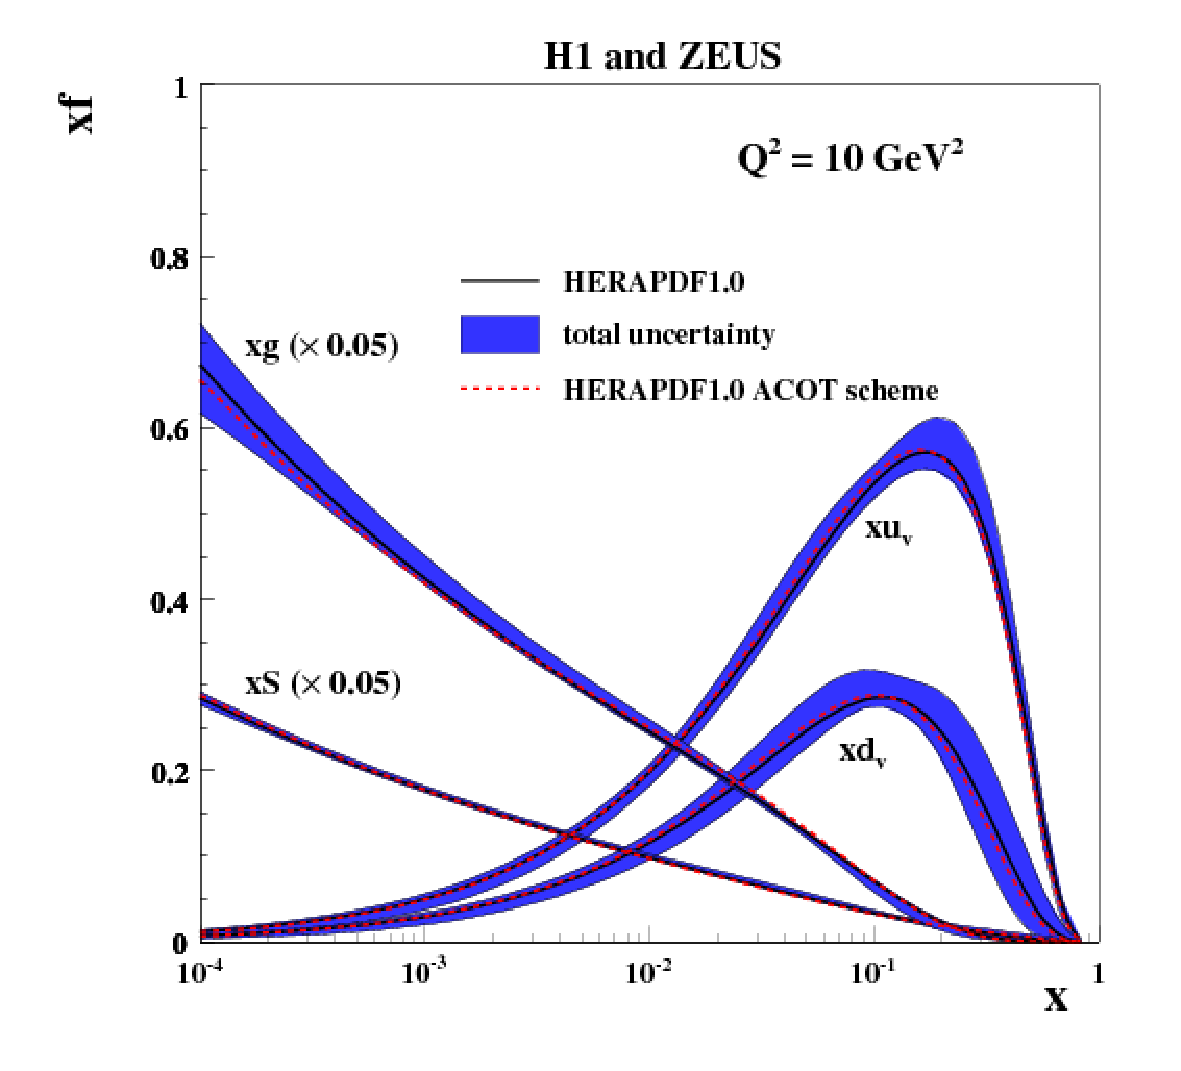
\includegraphics[width=8cm]{heraacot}
  \caption{Overview showing the $u-$ and $d$-valence, the total sea
    (scaled), and gluon (scaled) PDFs of the NLO HERAPDF1.0 set with their 
    total uncertainty at the scale of $Q^2 = 10\ \GeV^2$ obtained 
    using the TR' scheme and compared to the PDFs obtained with 
    the ACOT scheme using the $k$-factor technique (red).}
 \label{fig:acotrt}
\end{figure}



%\item 
%In the case of the DY processes the LO calculation described in section~\ref{dysection}
%is such that the PDFs can be factorised, allowing high speed calculations when 
%performing QCD fits over lepton rapidity data. In this case
%the factorised part of the expression which is independent of PDFs can be
%calculated only once for all minimisation iterations.
%The leading order code in \fitter package implements this 
%optimisation and uses fast convolution routines provided by
%\qcdnum. Currently the full width LO calculations are optimised 
%for lepton pseudorapidity and boson rapidity distributions with the
%possibility to apply lepton \(p_{\perp}\) cuts.
%making this procedure flexible to describe data.
%This flexibility allows the calculations to be performed within the phase space
%corresponding to the available measurement.
%The calculated LO cross sections are multiplied by
%$%k$-factors to obtain predictions at NLO.
%
%  \item In the case of the DY process a part of the LO calculation
%    described in Section~\ref{dysection} can be factored out such that
%    high speed calculations become possible when performing QCD fits
%    with lepton rapidity data. The part of the expression that can be
%    written as an extra factor is independent of the PDFs and needs to
%    be derived only once for all minimisation iterations. The
%    leading-order code in \fitter implements this optimisation and
%    uses fast convolution routines provided by \qcdnum. Currently, the
%    full width LO calculations are optimised for lepton pseudorapidity
%    and boson rapidity distributions with the possibility to apply
%    selection criteria to the lepton \pperp.
%    % making this procedure flexible to describe data.
%    This flexibility allows to perform the computations for
%    the phase space corresponding to each available measurement.
%    % The calculated leading order cross sections are multiplied by
%    % NLO or NNLO k-factors provided for corresponding data
%    % distributions.
%    The LO cross sections are then multiplied by $k$-factors to
%    obtain predictions at NLO\@.

\end{itemize}


%\vspace*{0.25cm}
%\item{\bf{}Fast grid technique:}
\subsection{Fast Grid Techniques}

  Fast grid techniques exploit the fact that iterative PDF fitting
  procedures do not impose completely arbitrary changes to the types
  and shapes of the parameterised functions that represent each PDF\@.
  Instead, it can be assumed that a generic PDF can be approximated by
  a set of interpolating functions with a sufficient number of
  strategically well-chosen support points. The quality, i.e.\ the
  accuracy of this approximation, can be tested and optimised by a
  number of means, the simplest one being an increase in the number of
  support points. Ensuring an approximation bias that is negligibly
  small for all practical purposes this method can be used to perform
  the time consuming higher-order calculation (see Eq.~\ref{eq:fact})
  only once for the set of interpolating functions. 
  The repetition of a cross section evaluation for
  a particular PDF set then is very fast and implies only sums over
  the set of interpolators multiplied by factors depending on the
  respective PDF\@. The described approach applies equally to
  processes involving one or two hadrons in the initial state as well
  as to the renormalisation and factorisation scale dependence in the
  convolution of the PDFs with the partonic cross section.

  This technique was pioneered in the \fastnlo
  project~\cite{Kluge:2006xs} to facilitate the inclusion of
  notoriously time consuming jet cross sections at NLO into PDF fits.
  The \applgrid~\cite{Carli:2010rw} package extended first a similar
  methodology to DY production. While differing in their interpolation
  and optimisation strategies, both packages construct tables with
  grids for each bin of an observable in two steps: In the first step
  the accessible phase space in the parton momentum fractions $x$ and
  the renormalisation and factorisation scales \mur and \muf is
  explored in order to optimize the table size. The second step
  consists of the actual grid construction and filling for the
  requested observables. Higher-order cross sections can then be
  restored very efficiently from the preproduced grids while varying
  externally provided PDF sets, \mur and \muf, or the strong coupling
  \asq\@. The approach can in principal be extended to arbitrary
  processes, but requires to establish an interface between the
  higher-order theory programs and the fast interpolation
  frameworks. Work in that direction is ongoing for both packages.
  They are described in some more detail in the following:

\begin{itemize}
  \item The \fastnlo project~\cite{Kluge:2006xs} has been interfaced
    to the \nlojetpp program~\cite{Nagy:1998bb} for the calculation of
    jet production in DIS~\cite{Nagy:2001xb} as well as 2- and 3-jet
    production in hadron-hadron collisions at
    NLO~\cite{Nagy:2003tz,Nagy:2001fj}. To demonstrate the
    applicability to higher-orders, threshold corrections at 2-loop
    order, which approximate the NNLO for the inclusive jet cross
    section, have been included into the framework as
    well~\cite{Wobisch:2011ij} following Ref.~\cite{Kidonakis:2000gi}.
    % KR: Maybe not necessary to include in a HERAFitter document
    % Recently it was shown~\cite{Kumar:2013hia,deFlorian:2013qia},
    % however, that in particular for the LHC the jet size $R$
    % dependence must be taken into account in these threshold
    % corrections.

    The latest version of \fastnlo~\cite{Britzger:2012bs} allows 
    creation of tables where renormalisation and factorisation scales
    can be chosen
    freely as a function of two pre-defined observables, e.g.\ jet
    transverse momentum \pperp and $Q$ for DIS\@. 
    \fastnlo can be obtained from~\cite{fastNLO:HepForge}, where
    numerous precalculated grid tables for jet cross sections can be
    downloaded as well. 
%    The latest release is compatible with \lhapdf
%    versions 5 or 6, includes the \as evolution package
%    \crundec~\cite{Schmidt:2012az}, and can also be linked to use the
%    \hoppet or \qcdnum evolution. The C++ library part can be accessed
%    via an optional Python interface.

    Dedicated \fastnlo libraries and tables required for comparison to
    particular datasets are included in the \fitter package. In this
    case, the evaluation of the strong coupling constant is taken
    consistently with the PDF evolution from the \qcdnum code. The
    interface to the \fastnlo tables from within \fitter was used in a
    recent CMS analysis, where the impact on the
    extraction of the PDFs from the inclusive jet cross section is
    investigated~\cite{cms:jets}. The influence on the gluon density by
    the CMS inclusive jet data is illustrated in Fig.~\ref{fig:cmsjet}.

\begin{figure}[!ht]
  \centering
  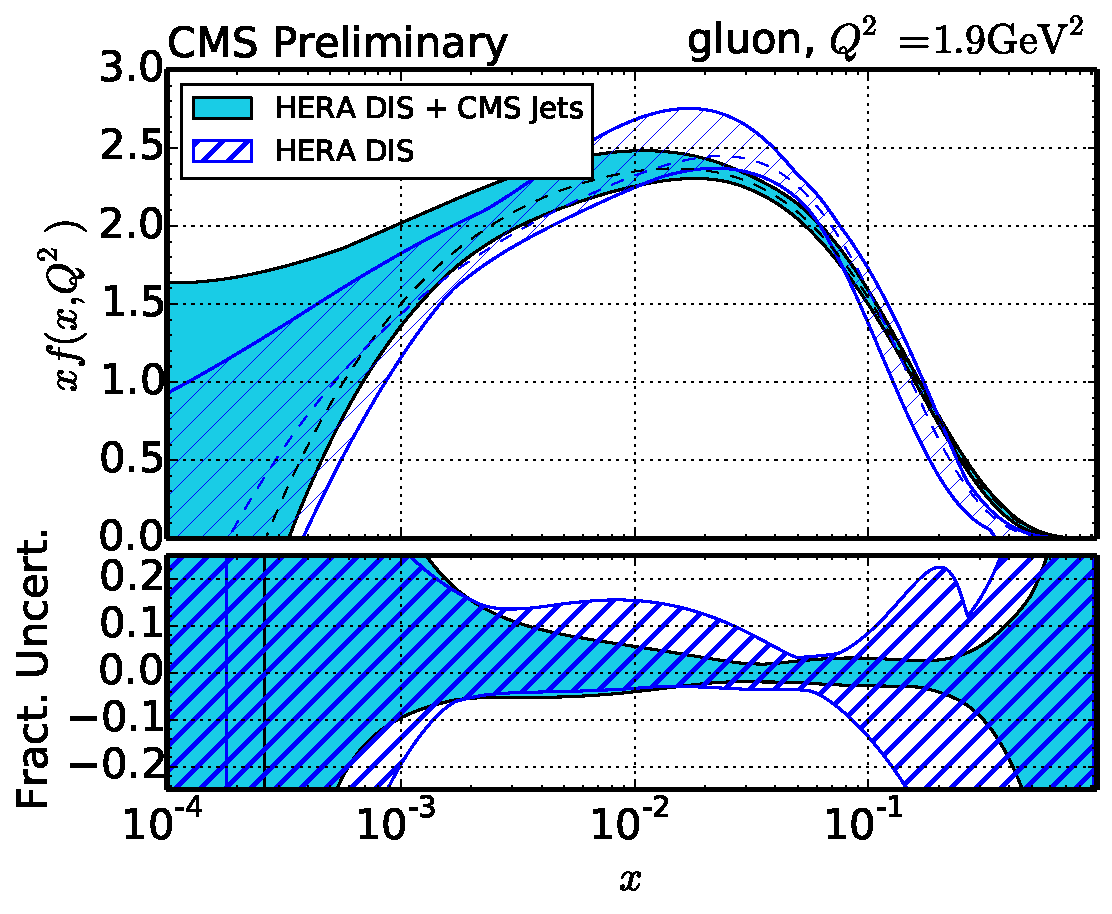
\includegraphics[width=8cm]{CMSjets}
  \caption{The gluon density as a function of $x$ as derived from
    HERA inclusive DIS data alone (cyan) and in combination with
    CMS inclusive jet data from 2011 (blue hatched), where bands
    represent the total uncertainty of the PDFs. The PDFs are
    shown at the starting scale $Q^2 = 1.9\ \GeV^2$.}
  \label{fig:cmsjet}
    \end{figure}

\item The \applgrid package~\cite{Carli:2010rw}, which is also
    available from~\cite{APPLGRID:HepForge}, in addition to
    the jet cross sections from \nlojetpp 
    in $pp(\bar p)$ and DIS processes, implements the calculations 
    of DY production. The look-up tables (also called grids) can be generated with
    modified versions of the \mcfm parton level generator for
    DY~\cite{Campbell:1999ah,Campbell:2000je,Campbell:2010ff}.  
%    The cross section observables and the grid parameters are 
%    defined in the \applgrid code.
    Alternative values of the strong coupling constant as well as 
    a posteriori variation of the renormalisation 
    and factorisation scales can be freely chosen in the calculation
    of the theory predictions with the \applgrid tables. 
    For NNLO predictions in \fitter $k$-factors can be applied.

    The \fitter interface to \applgrid was used by the ATLAS
    collaboration to extract the strange quark density of the proton
    from $W$ and $Z$ cross sections~\cite{atlas:strange}. An
    illustration of ATLAS PDFs extracted using the $k$-factors is shown in
    Fig.~\ref{fig:atlas} together with the comparison to global PDF
    sets CT10~\cite{CT10pdf} and NNPDF2.1~\cite{NNPDFpdf}.

\begin{figure}[!ht]
  \centering
  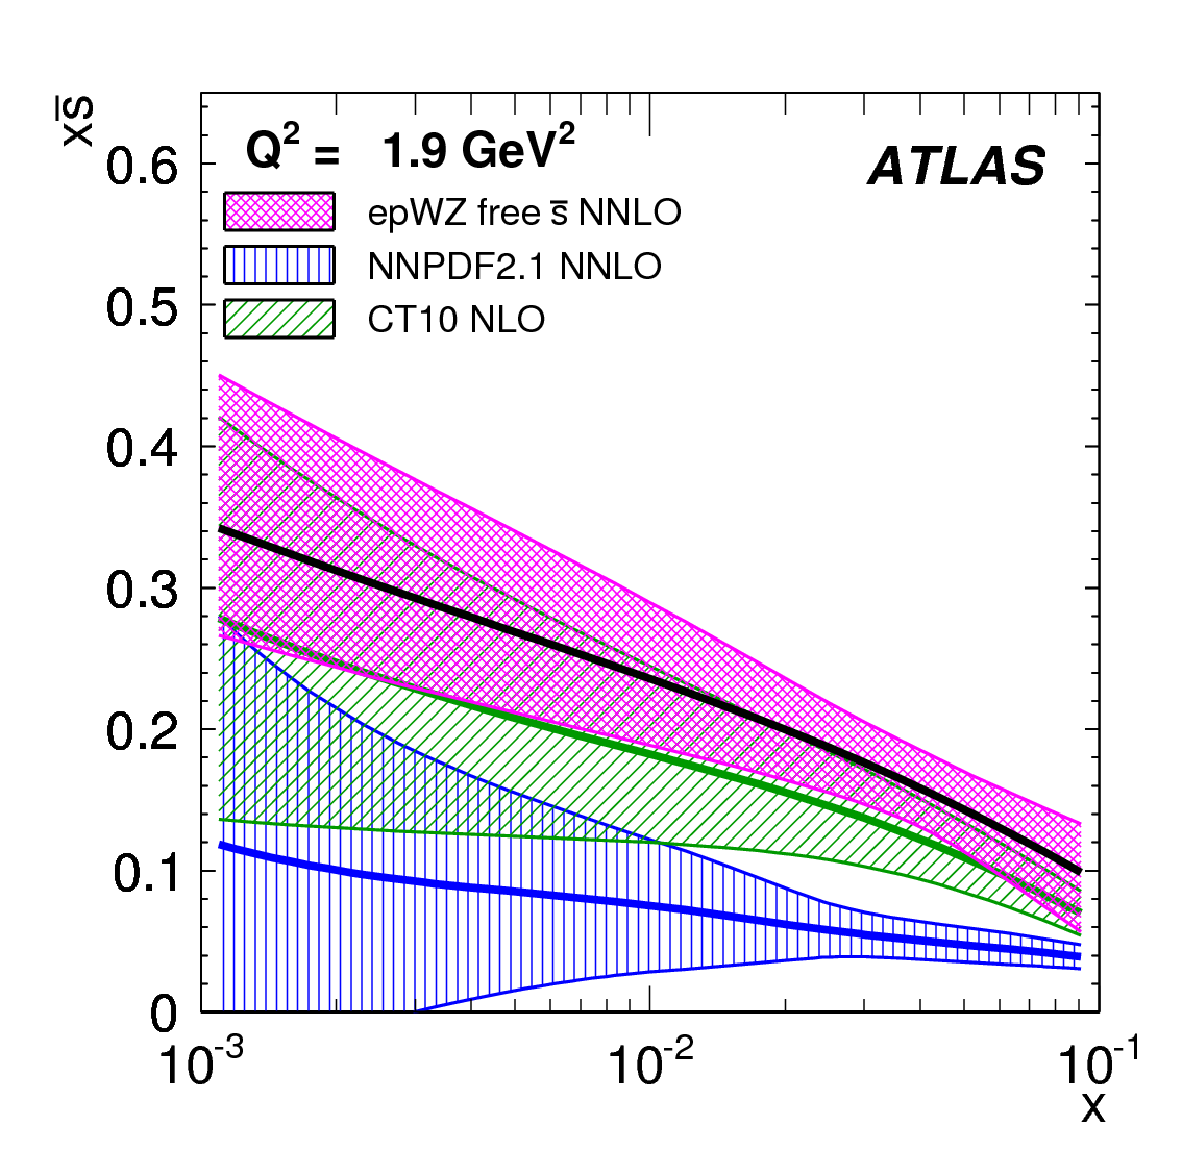
\includegraphics[width=8cm]{atlas.pdf}
  \caption{The strange anti-quark density versus $x$ for the ATLAS
    epWZ free sbar NNLO fit (magenta band) compared to predictions
    from NNPDF2.1 (blue hatched) and CT10 (green hatched) at $Q^2 = 1.9\ \GeV^2$.}
  \label{fig:atlas}
\end{figure}

%    \item The \applgrid~\cite{Carli:2010rw} package allows the fast computation 
%of NLO cross sections for particular processes for arbitrary sets of 
%proton parton distribution functions. The package implements
%calculations of DY production as well as jet production in $pp(\bar p)$
%collisions and DIS processes. 
%
%The approach is based on storing the perturbative coefficients
%of NLO QCD calculations of final-state observables measured
%at hadron colliders in look-up tables. The PDFs and the 
%strong couplings are included during the final calculations,
%e.g. during PDF fitting. The method allows 
%variation of factorisation and renormalisation scales in
%calculations.
%
%The look-up tables (grids) can be generated with modified versions
%of the \texttt{MCFM} parton level generator for DY~\cite{Campbell:1999ah,Campbell:2000je,Campbell:2010ff} 
%or \nlojetpp~\cite{Nagy:1998bb,Nagy:2001fj} code for NLO jet production.
%The model input parameters are pre-set as usual for \texttt{MCFM}, 
%while binning and definitions of the
%cross section observables are set in the \applgrid code.
%%as distributed with the full version of APPLGRID package.
%% NLO calculations
%%for the current analysis are performed with the help of APPLGRID
%%generated grids based on MCFM calculations. 
%%
%%APPLGRID supports an interface to the MCFM parton level generators,
%%hence model input parameters such as electroweak parameters
%%are in fact pre-set following the MCFM input steering card, while
%%binning and definitions of the observables for which the
%%differential cross sections are needed are set in the 
%%APPLGRID code. 
%%The grid parameters \(x_1, x_2\) and \(Q^2\) binning
%The grid parameters, \(Q^2\) binning
%and interpolation orders are also defined in the code.
%
%\applgrid constructs the grid tables in two 
%steps: {\it (i)} exploration of the phase space in order
%to optimize the memory storage and {\it (ii)} actual grid
%construction in the phase space corresponding to the 
%requested observables.
%The NLO cross sections are restored from the grids
%using externally provided PDFs, $\as$, factorization and 
%renormalization scales. For NNLO predictions $k$-factors can be applied.
%
%This method was used by the ATLAS collaboration in determining the strange 
%quark density of the proton from $W$ and $Z$ cross sections 
%together with HERA inclusive DIS data~\cite{atlas:strange}. 
%An illustration of PDFs extracted in~\cite{atlas:strange} using \applgrid method 
%and $k$-factors to correct from NLO to NNLO is shown 
%in Fig.~\ref{fig:atlas} togehter with the comparison to the global PDF sets 
%CT10~\cite{CT10pdf} and NNPDF2.1~\cite{NNPDFpdf}.
%
%\begin{figure}[!ht]
%   \centering
%   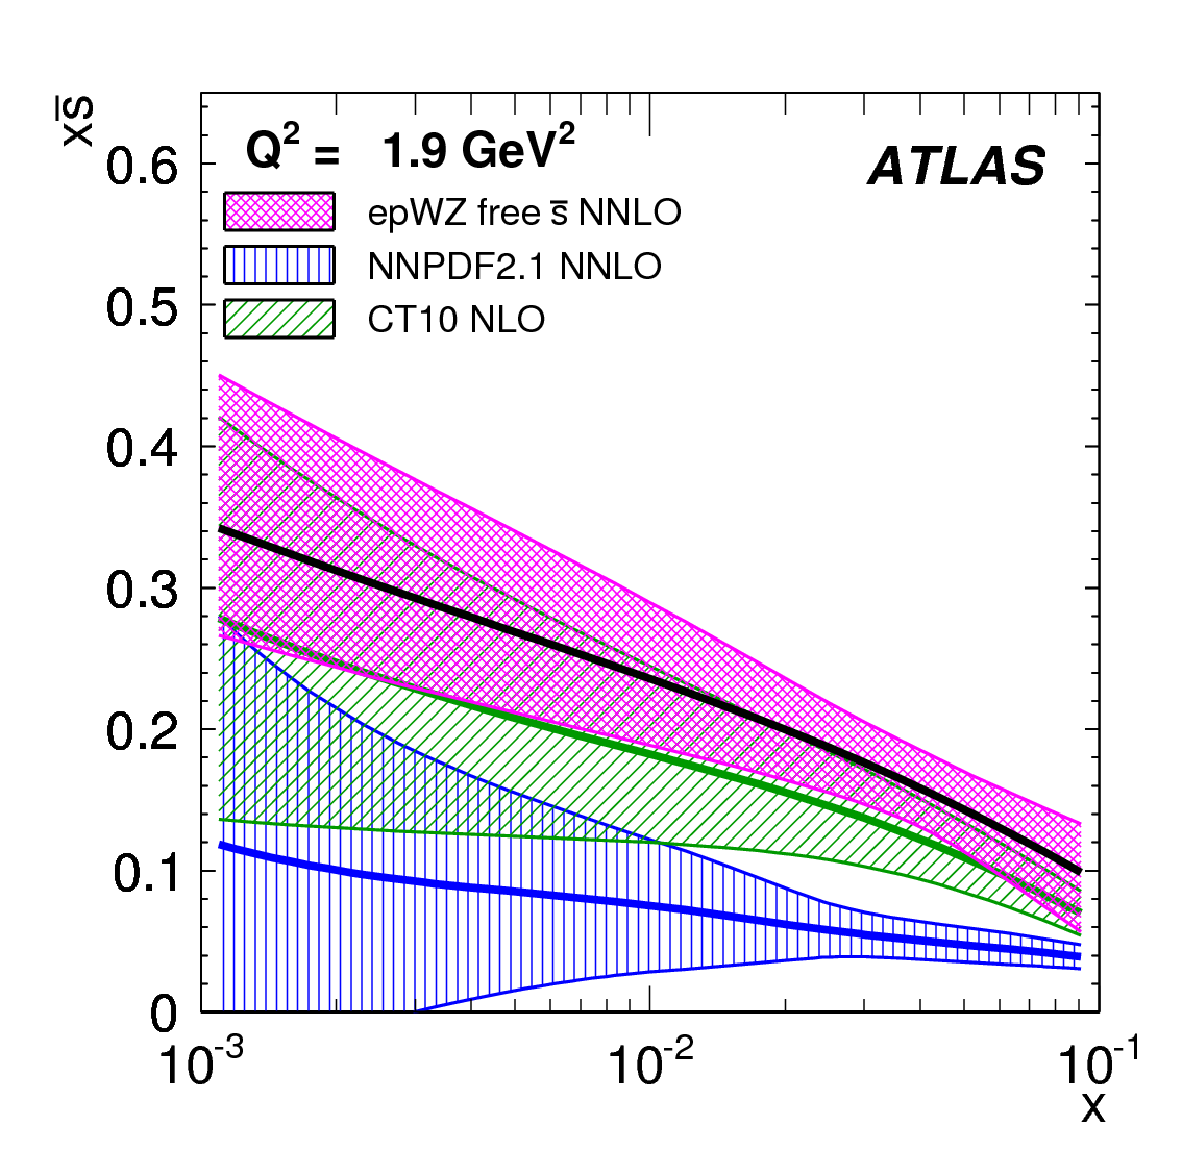
\includegraphics[width=8cm]{atlas.pdf}
%   \caption{The strange anti-quark density versus $x$ for the ATLAS epWZ free sbar NNLO fit (magenta band) compared to predictions from NNPDF2.1 (blue hatched) and CT10 (green hatched) at $Q^2= 1.9 \ \GeV^2$.}
% \label{fig:atlas}
%\end{figure}
%
%

\end{itemize}

%\end{description}

\subsection{Performance Optimisation}

%The above mentioned features make \fitter a powerful project that encapsulates 
%state of the art developments 
%from the most up-to-date theory developments 
%to debates on reaching the ultimate experimental precision. 
%on reaching the ultimate experimental precision. 

An important factor for a feasible QCD fit which is performed by iterative 
$\chi^2$ minimisation, is performance in terms of how long a calculation takes for each given data point.
The performance of the \fitter code is greatly improved with several special built-in options
including the $k-factor$ techniques (see section~\ref{sec:techniques}) and the grid techniques for the fast calculation of cross 
sections of particular processes for arbitrary sets of PDFs. There are also cache options, fast evolution kernels, and 
usage of the OpenMP (Open Multi-Processing) interface which allows
parallel applications of some of the heavy flavour scheme theory predictions in DIS. 
%{\bf please go over this, I have married two separate paragraphs that were in different places}





\section{Fit Methodology}
\label{sec:method}

%\fitter\ is a unique QCD fit platform that provides many options to the user to perform a quantitative assessment of impact level for a new data or new theoretical prediction. The quest on nailing down the uncertainties on PDFs have lead, on one hand, to highly precise measurements that are in need of careful handling of all provided sources of uncertainties, and on the other hand to numerous software packages that provide higher order calculations in QCD to match the precision of data.


When performing a QCD analysis to determine PDFs there are various assumptions and choices to be made concerning, for example, the functional form of the input parametrisation, the treatment of heavy quarks and their mass values, alternative theoretical calculations, alternative representations of the fit $\chi^2$, different ways of treating correlated systematic uncertainties.
%
 It is useful to be able to discriminate or quantify the effect of the chosen ansatz, within a common framework, and 
\fitter is optimally designed for such tests.
%
The methodology employed by \fitter  relies on a flexible and modular
framework that allows for independent integration of the state-of-the-art techniques, either related to the inclusion of a new theoretical calculation, or of new approaches to treat data and their uncertainties. 

In this section we describe the available options for the fit methodology in \fitter.
%ranging from the functional form used to parametrise PDFs and the choice of the form of the $\chi^2$ function, to different methods to assess the experimental uncertainties on extracted PDFs.
%
%list various types of functional forms used to parametrise PDFs, different definitions for  $\chi^2$ evaluation in extracting the PDF parameters which account for correlated and uncorrelated sources of experimental (or theoretical) uncertainties available in \fitter. 
In addition, as an alternative approach to a complete QCD fit, the Bayesian reweighting
method, which is also available in \fitter, is described.
\subsection{Functional Forms for PDF Parametrisation}
The PDFs can be parametrised using several predefined
functional forms and different flavour decompositions:
\paragraph{Standard Polynomials:} 
The standard polynomial form is the most commonly used. A polynomial functional form is used to parametrise the $x$-dependence of the PDFs, where index $j$ denotes each parametrised PDF flavour:
\begin{equation}
\centering
 xf_j(x) = A_j x^{B_j} (1-x)^{C_j} P_j(x).
\label{eqn:pdf_std}
\end{equation}
The parametrised PDFs are the valence distributions
$xu_v$ and $xd_v$, the gluon distribution $xg$, and the $u$-type and $d$-type sea,
% as constrained by HERA data alone,
$x\bar{U}$, $x\bar{D}$, where $x\bar{U} = x\bar{u}$, 
$x\bar{D} = x\bar{d} +x\bar{s}$ at the starting scale, which is 
chosen below the charm mass threshold. 
The form of polynomials $P_j(x)$ can be varied.
% depend on the style and is defined as a steerable parameter. 
The form $(1 + \epsilon_j \sqrt{x} + D_j x + E_j x^2)$
is used for the HERAPDF \cite{h1zeus:2009wt} 
with additional constraints relating to the flavour decomposition of the 
light sea. This parametrisation is termed HERAPDF-style. The polynomial can also
be parametrised in the CTEQ-style, $P_j(x)$ takes the form $e^{a_3x} (1 + e^{a_4} x + e^{a_5} x^2)$ and,
in contrast to  the HERAPDF-style, this is positive by construction.
QCD number and momentum sum rules are used to determine the normalisations $A$ for the valence and gluon
distributions, and the sum-rule integrals are solved analytically.
\paragraph{Bi-Log-Normal Distributions:} 
%A bi-log-normal distribution to parametrise the $x$ dependence of the PDFs is 
%also available in \fitter.
%parton distribution function of the proton.
This parametrisation is motivated by multi-particle statistics
%~\cite{hera-lhc:report2009}
and has the following functional form:
%\begin{center}
\begin{equation}
 xf_j(x)=a_j x^{p_j-b_j\log(x)}(1-x)^{q_j-d_j \log(1-x)}.
\label{eqn:bilog}
\end{equation}
%\end{center}
This function can be regarded as a generalisation of the standard polynomial form described above,
however, numerical integration of Eq.~\ref{eqn:bilog} is required in order to satisfy the QCD sum rules.
%In order to satisfy the QCD sum rules this parametric form requires numerical integration.
\paragraph{Chebyshev Polynomials:} 
A flexible parametrisation  based on the Chebyshev polynomials can be employed for the gluon and sea distributions.
Polynomials with argument $\log(x)$ are considered for better modelling the low-$x$ asymptotic of those PDFs. The polynomials are multiplied
by a factor of $(1-x)$ to ensure that they vanish as $x\to 1$. The resulting parametric form reads
\begin{eqnarray}
x g(x) &=& A_g \left(1-x\right) \sum_{i=0}^{N_g-1} A_{g_i} T_i \left(-\frac{\textstyle 2\log x - \log x_{\rm min} } {\textstyle \log x_{\rm min} } \right)\,, \label{eq:glu} \\
x S(x) &=& \left(1-x\right) \sum_{i=0}^{N_S-1} A_{S_i} T_i \left(-\frac{\textstyle 2\log x - \log x_{\rm min} } {\textstyle \log x_{\rm min} } \right)\,, \label{eq:sea} 
\end{eqnarray}
where $T_i$ are first-type Chebyshev polynomials of order $i$.
%The values of $N_{g,S}$ up to 15 are allowed, however, already
%starting from $N_{g,S}>5$ the fit quality is similar to the one based on
%the standard-polynomial parametrisation with a similar number of parameters.
The normalisation factor $A_g$ is derived from the momentum sum rule analytically.
Values of $N_{g,S}$ to $15$ are allowed, however the fit quality is already similar
to that of the standard-polynomial parametrisation from $N_{g,S} \ge 5$  and has a similar number of free parameters.
%
%where the sum runs over $i$ up to $N_{g,S}=15$ order Chebyshev polynomials of the first type $T_i$ for
%the gluon, $g$, and sea-quark, $S$, density, respectively. 
%The normalisation factor $A_g$ is defined from the momentum sum rule.
%%
%The advantages of this parametrisation are that the momentum sum rule can be evaluated analytically 
%and that for $N \ge 5$ the fit quality is already similar
%to the standard Regge-inspired parametrisation with a similar number of parameters.
%A study of the parametrisation uncertainty at low Bjorken $x \le 0.1$ for PDFs was presented 
%in~\cite{Chebyshev}. Figure~\ref{fig:cheb} shows the comparison of the 
%gluon density detemined from the HERA data  
%with the standard and the Chebyshev parametrisation.
%
%The low-$x$ uncertainties in the PDFs determined from the HERA data using different 
%parametrisatons were studied in Ref.~\cite{Chebyshev}.
Fig. \ref{fig:cheb} (taken from \cite{Chebyshev})
shows a comparison of the gluon density obtained with the parametrisation Eqs.~\ref{eq:glu}, \ref{eq:sea} to 
the standard-polynomial one, for $N_{g,S} = 9$.

%with a reduced parametrisation uncertainty. 
%An additional regularisation prior leads to a 
%significantly reduced uncertainty for $x \le 0.0005$.
\begin{figure}[!ht]
 \centering
%  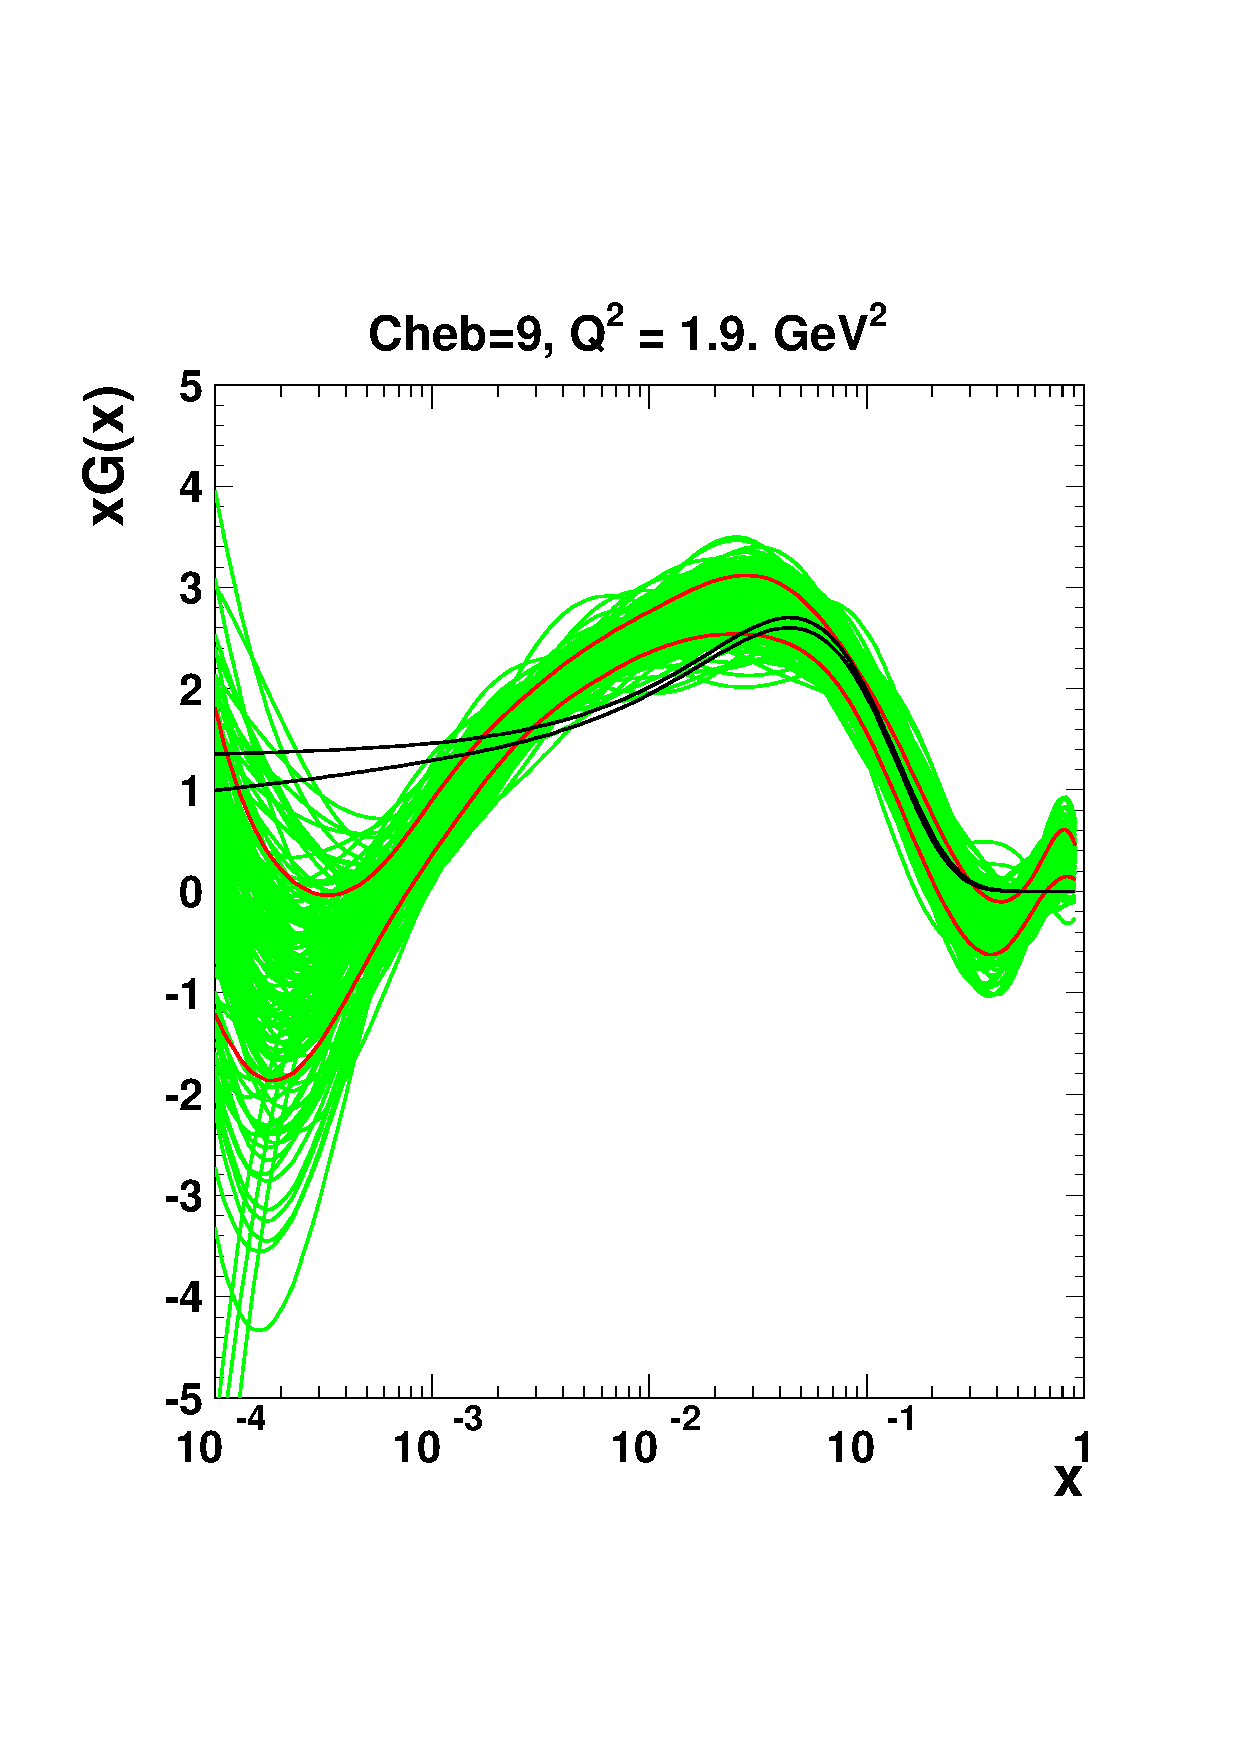
\includegraphics[width=5cm]{chebishev.pdf}
  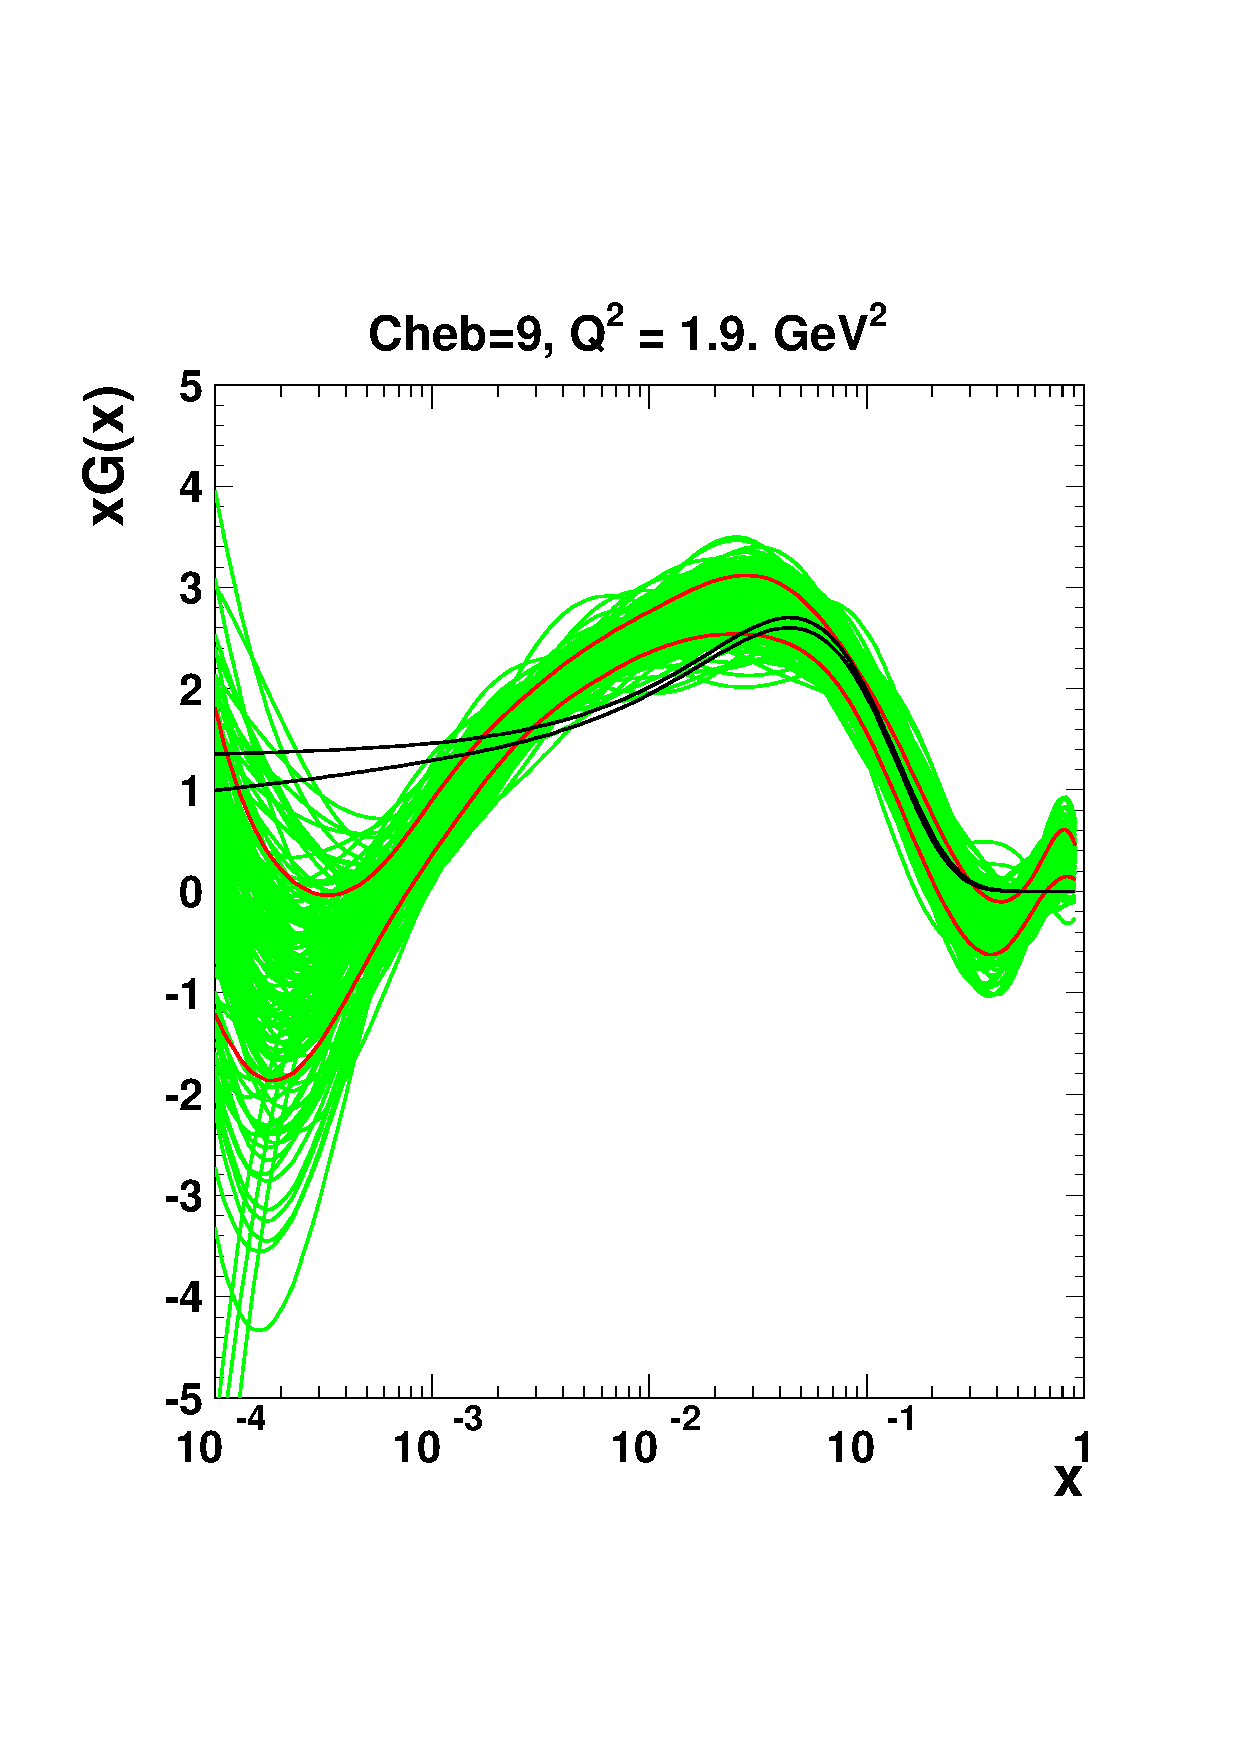
\includegraphics[trim=1cm 4cm 1cm 5cm, clip, width=6cm]{chebishev.pdf}
% \caption{Gluon PDF at the scale of $Q^2=1.9 \  \GeV^2$ for various values of the length-prior 
% weight $\alpha$ \cite{Chebyshev} using the Chebyshev parametrisation expanded to the 15th order.}
  \caption{The gluon density is shown at the starting scale. The black lines correspond to the uncertainty band of the gluon distribution using a standard parametrisation and it is compared to the case of the Chebyshev parametrisation \cite{Chebyshev}. The uncertainty band for the latter case is estimated using the Monte Carlo technique (see section \ref{sec:experimentalerrors}) with the green lines denoting fits to data replica.  Red lines indicate the standard deviation about the mean value of these replicas.}
 \label{fig:cheb}
\end{figure}

%
\paragraph{External PDFs:} \rm 
 \fitter also provides the possibility to access external PDF sets, which can be used to compute 
theoretical predictions for the cross sections for all the processes available in \fitter. 
This is possible via an interface to \lhapdf~\cite{lhapdf,lhapdfweb} providing access to the 
global PDF sets.
%available at different orders.
\fitter also allows to evolve PDFs from \lhapdf with \qcdnum using the corresponding grids as a starting scale.
%locally through the \fitter or taken as provided by the \lhapdf grids. 
Fig. \ref{fig:pdfs} illustrates a comparison of various PDFs accessed from \lhapdf as produced with the drawing 
tools available in \fitter.
%\end{description}
%
\begin{figure}[!ht]
   \centering
   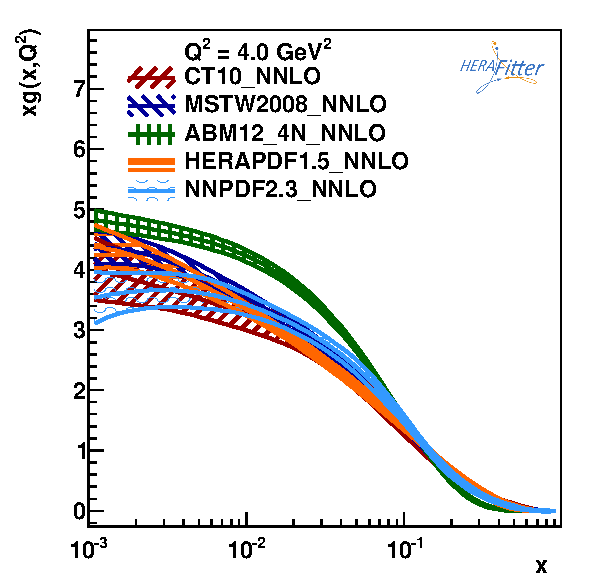
\includegraphics[width=8cm]{pdfs.pdf}
   \caption{The gluon PDF as extracted by various PDF groups at the scale of $Q^2=4 \ \GeV^2$, plotted using the drawing tools from \fitter.} 
 \label{fig:pdfs}
\end{figure}
%
\subsection{Representation of $\chi^2$}
\label{sec:chi2representation}

The PDF parameters are determined in \fitter by minimisation of the
$\chi^2$ function taking into account correlated and uncorrelated measurement uncertainties.
%The PDF parameters are extracted in a $\chi^2$ minimisation process.
%The construction of the $\chi^2$  accounts for the experimental uncertainties.
There are various forms of the $\chi^2$ 
e.g. using a covariance matrix or providing nuisance parameters to encode the dependence of 
each correlated systematic uncertainty for each measured data point.
%, different scaling options, etc. 
%In addition, there are various methods to deal with correlated systematic (or statistical) uncertainties. 
The options available in \fitter are the following.

\begin{description}
\item \it {Covariance Matrix Representation:} \rm
For a data point $\mu_i$ with a corresponding theory prediction $m_i$, 
the $\chi^2$ function 
can be expressed in the following form:
%
\begin{eqnarray}
\chi^2 (m)& = & \sum_{i,k}(m_i-\mu_i)C^{-1}_{ik}(m_k-\mu_k),
\end{eqnarray}
where the experimental uncertainties are given as a covariance matrix $C_{i,k}$ for measurements in bins $i$ and $k$.
%The $\chi^2$ function depends on the theory parameters $m^i$ 
%(denoted as the vector $\boldsymbol{m}$).
The covariance matrix $C_{ik}$ is given by a sum of statistical, uncorrelated and correlated systematic contributions: 
\begin{eqnarray}
C_{ik}& = & C^{stat}_{ik}+C^{uncor}_{ik}+C^{sys}_{ik}.
\end{eqnarray}
Using this representation one cannot distinguish the separate effect of each source of systematic uncertainty. 

\item \it{Nuisance Parameters Representation:} \rm
In this case the $\chi^2$ form is expressed as
\label{sec:nuisance_representation}
%\begin{eqnarray} 
%    \chi^2\left(\boldsymbol{m},\boldsymbol{b}\right) &= &  
% \sum_i \frac{\left[m^i - \sum_j \gamma^i_j m^i b_j  - {\mu^i} \right]^2}
%{ \textstyle \delta^2_{i,{\rm stat}}\mu^i \left(m^i -  \sum_j \gamma^i_j m^i b_j\right)
%  + \left(\delta_{i,{\rm uncor}}\,  m^i\right)^2} \nonumber \\
%  &+& \sum_j b^2_j.
%\label{eq:aven}
%\end{eqnarray}
%{ \small
%\begin{equation} 
%    \chi^2\left(\boldsymbol{m},\boldsymbol{b}\right) =   
% \sum_i \frac{\left[m^i - \sum_j \gamma^i_j m^i b_j  - {\mu^i} \right]^2}
%{ \textstyle \delta^2_{i,{\rm stat}}\mu^i \left(m^i -  \sum_j \gamma^i_j m^i b_j\right)
%  + \left(\delta_{i,{\rm uncor}}\,  m^i\right)^2}+ \sum_j b^2_j.
%\label{eq:aven}
%\end{equation}}
\begin{equation} 
    \chi^2\left(\boldsymbol{m},\boldsymbol{b}\right) =   
 \sum_i \frac{\left[ {\mu_i} - m_i \left( 1 - \sum_j \gamma^i_j b_j \right) \right]^2}
{ \textstyle \delta^2_{i,{\rm unc}}m_i^2 + \delta^2_{i,{\rm stat}}\, {\mu_i} m_i \left(1 - \sum_j \gamma^i_j b_j\right) }
  + \sum_j b^2_j,
\label{eq:aven}
\end{equation}
%
where, $\delta_{i,\rm stat}$ and $\delta_{i,\rm unc}$ are 
relative statistical and uncorrelated systematic uncertainties
of the measurement $i$.
%where, ${\mu_i}$ is the central value of the measurement $i$ 
% ${\mu_i}$ is the central value of the measurement $i$ 
%with its relative statistical $\delta_{i,\rm stat}$ 
%and relative uncorrelated systematic uncertainty $\delta_{i,\rm unc}$.
Further, $\gamma^i_j$ quantifies the sensitivity of the
measurement to the correlated systematic source $j$. 
The function $\chi^2$ depends in addition on
 the set of systematic nuisance parameters $b_j$.
This definition of the $\chi^2$ function assumes that
systematic uncertainties are proportional to the central prediction values
(multiplicative errors), whereas the statistical uncertainties scale 
with the square root of the expected number of events. 

During the $\chi^2$ minimisation, the nuisance parameters $b_j$ and the PDFs are determined, such that the effect of different sources of systematic uncertainties can be distinguished.
\\
%The nuisance parameters $b_j$ as well as the PDF parameters are free parameters of the fit. 
%The fit determines the best PDF parameters to
%the data taking into account correlated systematic shifts of the data. 

\item  \it{Mixed Form Representation:} \rm
In some cases, the statistical and systematic uncertainties of experimental data are provided in different forms.    
%It can happen that various parts of the systematic and statistical uncertainties are stored in different forms. 
For example, the correlated experimental systematic uncertainties are available as nuisance parameters
but the bin-to-bin statistical correlations are given in the form of covariance matrix.
%A situation can be envisaged when the correlated systematic experimental uncertainties are provided as nuisance parameters, but the statistical bin-to-bin correlations are given in the form of a covariance matrix. 
\fitter\ offers the possibilitiy to include such mixed forms of information. 
%information, when provided, as well as any other mixed 
for treating statistical, uncorrelated and correlated systematic uncertainties. 
%In the case of off-diagonal statistical uncertainties, the $\chi^2$ function
%\begin{equation} 
%\begin{eqnarray} 
% \label{eq:chi2gen}
%    \chi^2(\boldsymbol{m},\boldsymbol{b})& = & \sum_{ij} 
%         \left ( m^i - \sum_l \gamma^i_l(m^i)b_l - \mu^i \right)  C^{-1}_{{\rm stat.}~ij}(m^i,m^j) \nonumber \\  
%    && \left(  m^j - \sum_l \gamma^j_l(m^j)b_l - \mu^j \right) +  \sum_l b^2_l.
%\end{eqnarray}
%\end{equation}
%Here the scaling properties of the correlated systematic uncertainties 
%$\Gamma^i_j$ and
%of the covariance matrix $C_{{\rm stat.}~ij}$ are expressed as a dependence
%on $m_i$ and the dependence of $\delta_{\rm stat}$ on $b_j$ is ignored.
\end{description}
Any source of measured systematic uncertainty can be treated as additive or multiplicative. 
The statistical uncertainties can be included as additive or Poisson. Minimisation
with respect to nuisance parameters is performed analytically, however for more 
detailed studies of correlations individual nuisance parameters can be included in 
the \minuit minimisation.


\subsection{Treatment of the Experimental Uncertainties}
\label{sec:experimentalerrors}


Three distinct methods for propagating experimental uncertainties to PDFs are implemented in \fitter and reviewed here:
%\fitter\ provides three methods for assessing the experimental uncertainties on PDFs: 
the Hessian, Offset, and Monte Carlo method.
%Figure \ref{fig:error} illustrates the difference between the Hessian and Monte-Carlo methods both of which can be applied and plotted with \fitter.
%\begin{figure}[!ht]
%   \centering
%   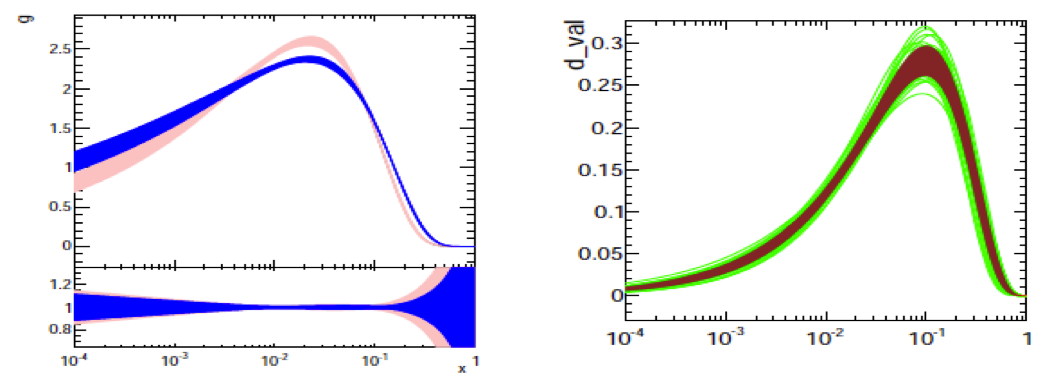
\includegraphics[width=8cm]{error.pdf}
%   \put (-206, 68) {Hessian}
%   \put (-86, 68) {Monte Carlo}
%   \caption{Differences in the experimental uncertainties on the gluon (left) and d-valence quark (right) densities extracted 
%       through different methods in \fitter: Hessian(left) versus Monte Carlo (right).} 
% \label{fig:error}
%\end{figure}
\begin{description}
\item \it{Hessian (Eigenvector) method:} \rm
The PDF uncertainties reflecting the uncertainties in experimental data are estimated by 
examining the shape of $\chi^2$ in the neighbourhood of the minimum \cite{Pumplin:2001ct}.
%The technique developed in~\cite{Pumplin:2001ct} presents an estimate of PDF uncertainties 
%reflecting the experimental precision of data used in the QCD fit by examining the behavior 
%of $\chi^2$ in the neighborhood of the minimum. 
Following approach of Ref. \cite{Pumplin:2001ct}, the Hessian matrix is defined by the second 
derivatives of $\chi^2$ on the fitted PDF parameters. The matrix is diagonalised and the 
Hessian eigenvectors are computed. 
Due to orthogonality, these vectors correspond to independent sources of
uncertainty in the obtained PDFs.
%
%This is known as the Hessian or error matrix method. 
%The Hessian matrix is built by the second derivatives of $\chi^2$ at the minimum. 
%The Hessian matrix is diagonalised through an iterative procedure and its PDF eigenvectors
%are obtained, which correspond to the orthogonal sources of uncertainties on the obtained PDF.

\item \it{Offset  method:} \rm
The Offset method \cite{Botje:2001fx} uses
%Another method to propagate the correlated systematic experimental uncertainties from 
%the measurements to PDFs \cite{Botje:2001fx} is Offset method.
%, which has the practical advantage that it does not require the inversion of a large measurement covariance matrix.
%
the $\chi^2$ function for the central fit, however only
uncorrelated uncertainties are taken into account. 
The goodness of the fit can no longer be judged from the $\chi^2$ since correlated uncertainties are ignored. 
The correlated uncertainties are propagated into the PDF uncertainties by performing variants 
of the fit with the experimental data varied by $\pm 1 \sigma$ from the central value  
for each systematic source.
The resulting deviations of the PDF parameters from the ones obtained in the central 
fit are statistically independent, and they can be combined in quadrature to arrive at the total 
PDF systematic uncertainty.
%
%Instead, the correlated systematic uncertainties of the measurement are used to estimate 
%the errors on the PDF parameters as follows.
%The cross section is varied by $\pm 1 \sigma$ from the central value 
%for each systematic source and the fit is performed. 
%After this has been done for all sources, the 
%resulting deviations of each of these fits from the central PDF parameters are added in quadrature. 

The uncertainties estimated by the offset method are generally larger than 
those from the Hessian method.
\\
%as the offset method does not use the information on correlated systematic uncertainties 
%in the central fit.

\item \it{Monte Carlo method:} \rm
The Monte-Carlo technique \cite{Giele:1998gw, mcmethod2} can also be used to determine PDF uncertainties.
The uncertainties are estimated using pseudo-data replicas (typically $>100$) 
randomly generated from the measurement central values and their systematic and statistical uncertainties 
taking into account all point-to-point correlations.
%
The QCD fit is performed for each replica and the PDF central values and their 
experimental uncertainties are estimated from the distribution of the PDF parameters obtained in these fits, by taking 
the mean values and standard deviations over the replicas.
%
%The preparation of the data is repeated for large $N$ ($>100$ times) and for each of these replicas a QCD fit is performed. 
%The PDF central values and experimental uncertainties are estimated using the mean values 
%and standard deviations over the replicas.

%The MC method represents one of the main concepts of the NNPDF group.
The MC method has been checked against the standard error estimation of the PDF uncertainties obtained by the Hessian method. 
A good agreement was found between the methods provided that Gaussian distributions of statistical and systematic uncertainties are assumed in the MC 
approach~\cite{hera-lhc:report2009}.
%when employing for the MC approach the assumption that uncertainties 
%(statistical and systematic) follow Gaussian distribution~\cite{hera-lhc:report2009}. 
A comparison is illustrated in Fig.~\ref{fig:mchessian}. 
Similar findings were reported by the MSTW global analysis~\cite{Watt:2012tq}. 
\begin{figure}[!ht]
 \centering
%  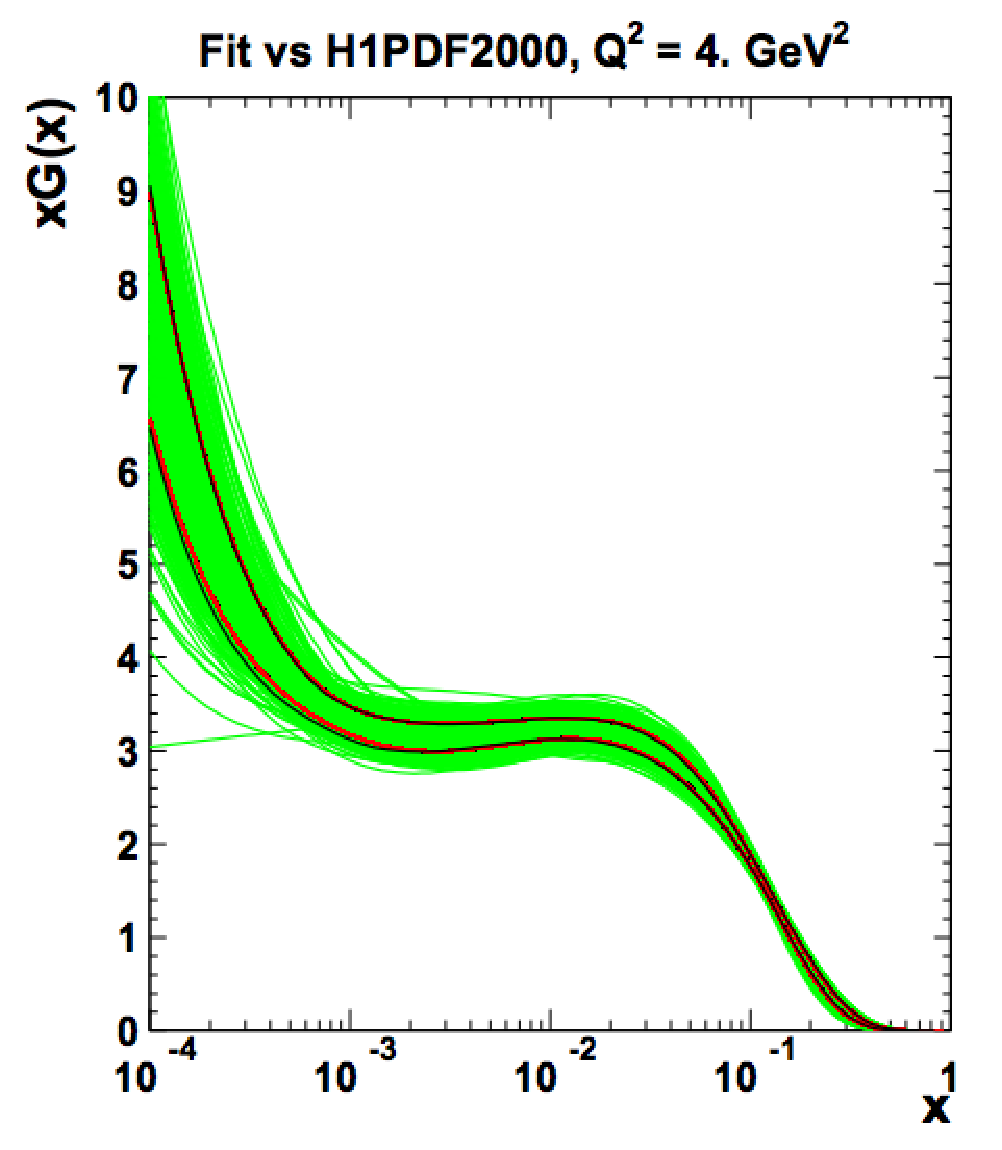
\includegraphics[width=7cm,height=7cm]{mchessian.pdf}
  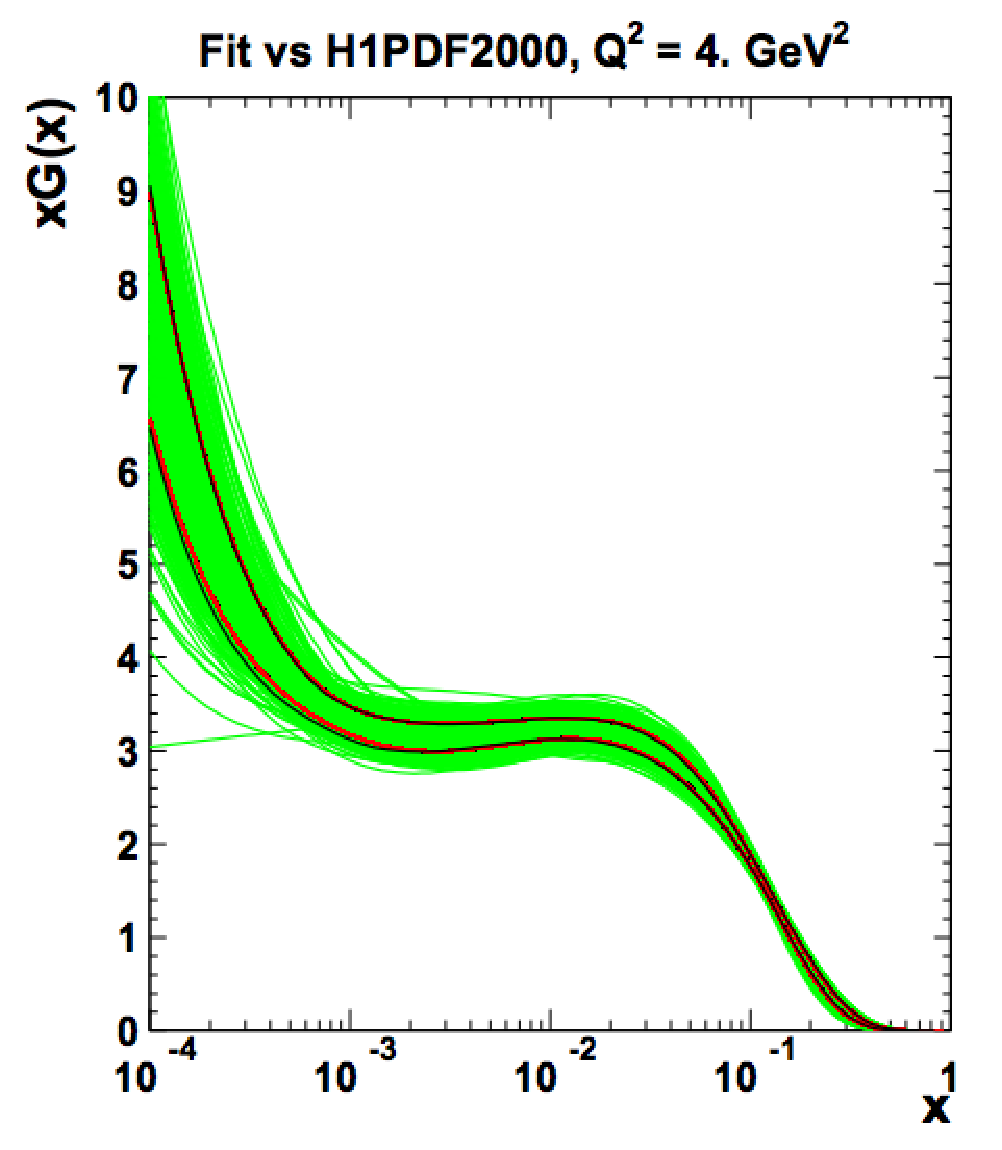
\includegraphics[trim=1cm 4cm 1cm 5cm, clip, width=6.3cm]{mchessian.pdf}
  \caption{Comparison between the standard error calculations as employed by the Hessian approach (black lines) 
           and the MC approach (with more than 100 replicas) assuming Gaussian distribution for uncertainty 
           distributions, shown here for each replica 
          (green lines) together with the evaluated standard deviation (red lines) \cite{hera-lhc:report2009}.
          The black lines in the figure are difficult to see because agreement of the methods is so good that thet are mostly covered by the red lines.}
  \label{fig:mchessian}        
\end{figure}
%

Since the MC method requires large number of replicas, the eigenvector representation 
is a more convenient way to store the PDF uncertainties.
It is possible to transform MC to eigenvector
representation as shown by \cite{Gao:2013bia}. Tools to perform this transformation are provided with \fitter and were 
recently employed for the representation of correlated sets of PDFs at different perturbative order \cite{hfcorrpaper}.
%
\end{description}
%
The nuisance parameter representation of $\chi^2$ in Eq.~\ref{eq:aven} is derived assuming 
symmetric experimental errors, however, the published systematic uncertainties are 
often asymmetric.
%Generally, the experimental uncertainties using nuisance parameters are 
%symmetrised when QCD fits 
%are performed, however often the provided uncertainties are rather asymmetric.
\fitter provides the possibility to use asymmetric systematic uncertainties.
The implementation relies on the assumption that 
asymmetric uncertainties can be described by a parabolic function.
The nuisance parameter in Eq.~\ref{eq:aven} is modified as follows
\begin{equation}
  \gamma^i_{j} \to \omega^i_{j}b_j + \gamma^i_{j},
\end{equation}
where the coefficients $\omega^i_{j}$, $\gamma^i_{j}$ are defined  
from the maximum and minimum shifts of the cross sections due to variaion of the systematic uncertainty $j$, 
$S_{ij}^{\pm}$,
\begin{equation}
  \omega^i_{j}=\frac{1}{2}\left(S_{ij}^{+}+S_{ij}^{-}\right), \\
  \gamma^i_{j}=\frac{1}{2}\left(S_{ij}^{+}-S_{ij}^{-}\right). 
\end{equation}
%For this case the definition of the $\chi^2$ from Eq.~\ref{eq:aven} is extended with the parabolic approximation 
%for asymmetric uncertainties, such that the expected cross section is adjusted to be
%\begin{equation}
%  m_i(1-\sum_j \gamma^i_{j} b_j) \to 
%m_i\left(1-\sum_j b_j(\omega^i_{j}b_j + \gamma^i_{j})\right).
%\end{equation}
%%The minimisation is performed using fixed number of iterations (typically ten), with rapid convergence.





\subsection{Treatment of the Theoretical Input Parameters}
\label{sec:theoryerr}

The results of a QCD fit depend not only on the input data but also on the 
input parameters used in the theoretical calculations. Nowadays, PDF groups 
address the impact of the choices of theoretical parameters by providing
alternative PDFs with different choices of the mass of the charm quarks, $m_c$, 
mass of the bottom quarks, $m_b$, and the value of $\asmz$. 
Other important aspects are the choice of the functional form for the PDFs at the 
starting scale and the value of the starting scale itself. \fitter provides the
possibility of different user choices of all these inputs to the theory.
%a platform in which such choices can readily be varied within a common framework.

\subsection{Bayesian Reweighting Techniques}

As an alternative to performing a full QCD fit, \fitter allows the user to assess the impact of including new
data in an existing fit using the Bayesian Reweighting technique. The method
provides a fast estimate of the impact of new data on PDFs. 
Bayesian Reweighting was first proposed for PDF sets delivered in the form of MC replicas by~\cite{Giele:1998gw} and further developed by the NNPDF Collaboration~\cite{Ball:2011gg,Ball:2010gb}. 
More recently, a method to perform Bayesian Reweighting studies starting from PDF fits for which uncertainties
are provided in the eigenvector representation has been also developed~\cite{Watt:2012tq}. The latter is 
based on generating replica sets by introducing Gaussian fluctuations on the central PDF set with a variance 
determined by the PDF uncertainty given by the eigenvectors. Both reweighting methods are implemented in \fitter.

The Bayesian Reweighting technique relies on the fact that MC replicas of a PDF set give 
a representation of the probability distribution in the space of PDFs. In particular, the PDFs are represented 
as ensembles of $N_{\rm rep}$ equiprobable ({\em i.e.} having all weight equal to unity) replicas, $\{f\}$. 
The central value for a given observable, $\mathcal{O}(\{f\})$, is computed as the average of the 
predictions obtained from the ensemble as
\begin{equation}
\langle\mathcal{O}(\{f\})\rangle =  \frac{1}{N_{\mathrm{rep}}} \sum_{k=1}^{N_{\mathrm{rep}}} \mathcal{O}(f^{k}),
\end{equation}
and the uncertainty as the standard deviation of the sample.

Upon inclusion of new data the prior probability distribution, given by the prior PDF set, is updated according
to Bayes Theorem such that the weight of each replica, $w_k$, is updated according to
\begin{equation}
 w_k = \frac{(\chi^2_k)^{\frac{1}{2} (N_{\mathrm{data}}-1) } e^{-\frac{1}{2}\chi^2_k}}
          { \frac{1}{N_{\mathrm{rep}}} \sum^{N_{\mathrm{rep}}}_{k=1}(\chi^2_k)^{\frac{1}{2}(N_{\mathrm{data}}-1)} e^{-\frac{1}{2}\chi^2_k}  },
\end{equation}
where $N_{\mathrm{data}}$ is the number of new data points, $k$ denotes the specific replica for which the 
weight is calculated and $\chi^2_k$ is the chi-square of the new data obtained using the $k$-th PDF replica.
%{\small
%\begin{equation}
%% \chi^2 (y,\mathrm{PDF}_k) = \sum_{i,j=1}^{N_{\mathrm{data}}} (y_i - y_i(\mathrm{PDF}_k)) \sigma^{-1}_{ij} (y_j-y_j(\mathrm{PDF}_k))\,. 
% \chi^2 (m,\mathrm{PDF}_k) = \sum_{i,j=1}^{N_{\mathrm{data}}} \left( m_i - m_i(\mathrm{PDF}_k)\right) \sigma^{-1}_{ij} (m_j-m_j\left(\mathrm{PDF}_k)\right)\,. 
%\end{equation}
%}
Given a PDF set and a corresponding set of weights, which describes the impact of the
inclusion of new data, the prediction for a given observable after inclusion of the new data can be computed as the {\em weighted} average,
\begin{equation}
\langle\mathcal{O}(\{f\})\rangle =  \frac{1}{N_{\mathrm{rep}}} \sum_{k=1}^{N_{\mathrm{rep}}} w_k \mathcal{O}(f^{k}).
\end{equation}

To simplify the use of reweighted set, an unweighted set ({\em i.e.} a set of equiprobable replicas which incorporates 
the information contained in the weights) is generated according to the unweighting procedure described in~\cite{Ball:2011gg}. 
The number of effective replicas of a reweighted set is measured by its Shannon 
Entropy~\cite{Ball:2010gb}
\begin{equation}
\label{eq:shannon}
N_\mathrm{eff}\equiv 
\exp\left\{\frac{1}{N_\mathrm{rep}}\sum_{k=1}^{N_\mathrm{rep}}w_k\ln(N_\mathrm{rep}/w_k)\right\}\,,
\end{equation}
which corresponds to the size of a refitted equiprobable replica set containing the same amount of information. 
This number of effective replicas, $N_\mathrm{eff}$, gives an indicative measure of the optimal size of an 
unweighted replica set produced using the reweighting/unweighting procedure. No extra information is 
gained by producing a final unweighted set that has a number of replicas (significantly) larger than 
$N_\mathrm{eff}$.  If $N_\mathrm{eff}$ is much smaller than the original number of replicas the new data have great impact, however it is unreliable to use the new reweghted set. Instead a full refit should be performed.

%On the one hand there is no reason in generating a final unweighted set that has a number of replicas
%(significantly) larger than $N_\mathrm{eff}$ as no extra information is gained. On the other hand it is
%advisable to start from a prior PDF set which has as many replicas as possible in order to have a more
%accurate posterior set at the end of the reweighting procedure.






\section{Alternatives to DGLAP Formalism}
\label{sec:alternative}


%\subsection{Alternative to DGLAP DIS models}
QCD calculations based on the DGLAP~\cite{Gribov:1972ri,Gribov:1972rt,Lipatov:1974qm,
Dokshitzer:1977sg,Altarelli:1977zs} evolution equations are very successful in describing
all relevant hard scattering data in the perturbative region $Q^2 \gtrsim $ few $ \GeV^2$.
At small-$x$ ($x <$ 0.01) and small-$Q^2$ DGLAP dynamics may be modified
 by saturation and other (non-perturbative) higher-twist effects.
%
Different approaches alternative to the DGLAP formalism can be used to analyse DIS data in \fitter.
These include several dipole models and the use of 
transverse momentum dependent, or unintegrated PDFs (uPDFs).

\subsection{Dipole Models}

The dipole picture provides an alternative approach to proton-virtual photon
 scattering at low $x$ which can be applied to both inclusive and 
diffractive processes.
 In this approach, the virtual photon fluctuates into a $q\bar q$ (or $q\bar q g$) 
 dipole which interacts with the proton~\cite{NNZ:91,Mueller:1993rr}.  
The dipoles can be considered as quasi-stable quantum mechanical states, which have very long 
life time $\propto 1/m_p x\;$ and a size which is not changed by scattering with the proton.
The dynamics of the interaction are embedded in a dipole scattering amplitude.

Several dipole models, which assume different behaviours of the dipole-proton 
cross section, are implemented in \fitter:
the Golec-Biernat-W\"usthoff (GBW)
dipole saturation model~\cite{Golec-Biernat:1998js},
a modified GBW model which takes into account the effects of  
DGLAP evolution, termed the Bartels-Golec-Kowalski (BGK) dipole model~\cite{Bartels:2002cj}
and the colour glass condensate approach to the high parton density 
regime, named the Iancu-Itakura-Munier (IIM) dipole model~\cite{Iancu:2003ge}.
%\end{itemize}

%\begin{description}
\paragraph{GBW model:} \rm
In the GBW model the dipole-proton cross section $\sigma_{\text{dip}}$ is given by
\begin{equation}
\label{eGBW}
   \sigma_{\text{dip}}(x,r^{2}) = \sigma_{0} \left(1 - \exp \left[-\frac{r^{2}}{4R_{0}^{2}(x)} \right]\right),
\end{equation}
where $r$ corresponds to the transverse separation between the quark and the antiquark, and $R_{0}^{2}$
 is an $x$-dependent scale parameter which represents the spacing of the gluons in the proton. 
$R_{0}^{2}$ takes the form, $R_0^2(x) = (x/x_0)^\lambda  1/ {\rm \GeV}^{2}$, and is called the saturation radius.
The cross-section normalisation $\sigma_0$, $x_0$, and $\lambda$ are parameters 
of the model fitted to the DIS data.
This model gives exact Bjorken scaling when the dipole size $r$ is small.
%%%%
 
\paragraph{BGK model:} \rm
The BGK model is a modification of the GBW model assuming that the
spacing $R_0$ is inverse to the gluon distribution and taking
into account the DGLAP evolution of the latter.
The gluon distribution, parametrised at some starting scale by Eq.~\ref{eqn:pdf_std}, 
is evolved to larger scales using DGLAP evolution.

\paragraph{BGK model with valence quarks:} \rm
The dipole models are valid in the low-$x$ region only, where the valence quark contribution to the total proton momentum 
is 5\% to 15\% for $x$ from 0.0001 to 0.01 \cite{Collaboration:2010ry}.
%, of the order of 5\%. 
The inclusive HERA measurements have a precision which is better than 2$\%$. 
Therefore, \fitter provides the option of taking into account the contribution of the valence quarks
%
%therefore, in \fitter the contribution of the valence quarks can be taken into account~\cite{Luszczak:2013rxa}.

\paragraph{IIM model:} \rm
The IIM model assumes an expression for the dipole cross section which is based on the 
Balitsky-Kovchegov equation~\cite{Balitsky:1995ub}. The explicit formula for $\sigma_{\text{dip}}$ 
can be found in~\cite{Iancu:2003ge}. 
The alternative scale parameter $\tilde{R}$, $x_{0}$ and $\lambda$ are fitted parameters of the model.

\subsection{Transverse Momentum Dependent PDFs}


\def\kt{\ensuremath{k_t}}
\def\pt{\ensuremath{p_t}}


QCD calculations of multiple-scale processes  and complex final-states
can necessitate the use of transverse-momentum dependent (TMD)~\cite{Collins:2011zzd}, or 
unintegrated parton distribution and parton decay 
functions~\cite{Aybat:2011zv,Buffing:2013eka,Buffing:2013kca,Buffing:2012sz,Mulders:2008tf,Jadach:2009gm,Hautmann:2009zzb,Hautmann:2012pf,Hautmann:2007gw}.   
TMD factorisation has been proven recently \cite{Collins:2011zzd} for inclusive DIS. TMD factorisation has also been proven in the high-energy (small-$x$) limit \cite{Catani:1990xk,Collins:1991ty,Hautmann:2002tu} for 
particular hadron-hadron scattering processes, like heavy flavour, vector boson and Higgs production.
  
In the framework of high-energy factorisation~\cite{Catani:1990xk,Catani:1990eg,Catani:1993ww} 
the DIS cross section can be written as a convolution in 
both longitudinal and transverse momenta of the TMD parton distribution function 
${\cal A}\left(x,\kt,\mu_{F}^2\right)$    
 with the off-shell parton scattering matrix elements as follows 
\begin{equation}
 \sigma_j (x, Q^2) = \int_x^1  
d z \int d^2k_t \ 
\hat{\sigma}_j(x,Q^2,{z},k_t) \ 
 {\cal  A}\left( {z} ,\kt, \mu_{F}^2 \right), 
\label{kt-factorisation}
\end{equation}
where  the DIS cross sections 
$\sigma_j$($j= 2 , L$) 
are related to the  structure functions $F_2$ and $F_L$ 
by 
$\sigma_j = 4 \pi^2 F_j / Q^2$, and   
the hard-scattering kernels ${\hat \sigma}_j$ of Eq.~\ref{kt-factorisation}
are $k_t$-dependent. 

The factorisation formula in Eq. \ref{kt-factorisation}
allows resummation of   
logarithmically enhanced small-$ x  $ contributions  
 to all orders in perturbation theory,  
both in the  hard 
scattering coefficients and 
in  the parton evolution, fully taking into account the 
dependence on the factorisation scale $\mu_F$ and on the 
factorisation scheme~\cite{Catani:1994sq,Catani:1993rn}.  


Phenomenological applications of this approach require 
matching of small-$ x  $ contributions with  finite-$x$ contributions.  To this end, 
the evolution  of the 
transverse momentum dependent gluon density 
${\cal  A} $ is obtained  by combining    the resummation of  small-$x$ logarithmic 
corrections~\cite{Lipatov:1996ts,Fadin:1975cb,Balitsky:1978ic}   with   medium-$x$  and large-$x$ 
contributions to parton  splitting~\cite{Gribov:1972ri,Altarelli:1977zs,Dokshitzer:1977sg} according to the 
CCFM  evolution equation~ \cite{\CCFM}. \textcolor{red}{Sea quark
contributions \cite{Hautmann:2012sh} are not yet
included at transverse momentum dependent level.} 
%\cite{Ciafaloni:1987ur,Catani:1989sg,Marchesini:1994wr}.


The cross section $\sigma_j$, ($j= 2 , L$) is calculated in a FFN   scheme,  using 
the boson-gluon fusion process ($\gamma^* g^* \to q \bar{q}$). The masses of the 
quarks are explicitly included as  parameters of the model.
In addition to $\gamma^* g^* \to q\bar{q}$,  the contribution from valence quarks is included 
via $\gamma^* q \to q$   by using  a CCFM evolution of 
valence quarks~\cite{Deak:2010gk,Deak:2011ga,Hautmann:2013tba}. 

%where the DIS cross sections 
%$\sigma_j$ ($j= 2 , L$) are related to the  structure functions $F_2$ and $F_L$.
%The hard-scattering kernels ${\hat \sigma}_j$ of Eq.~\ref{kt-factorisation},    are $k_t$-dependent and the evolution  of the 
%transverse-momentum dependent gluon distribution 
%${\cal A} $ is obtained by combining the resummation of small-$x$ logarithmic 
%contributions \cite{Lipatov:1996ts,Fadin:1975cb,Balitsky:1978ic} with medium-$x$ and large-$x$ 
%contributions to parton  splitting~\cite{Gribov:1972ri,Altarelli:1977zs,Dokshitzer:1977sg} according to the 
%CCFM evolution equation~\cite{Ciafaloni:1987ur,Catani:1989sg,Marchesini:1994wr}.
  
%The factorisation formula (\ref{kt-factorisation})  
%allows resummation of logarithmically enhanced small-$x$ contributions  
%to all orders in perturbation theory,  
%both in the  hard-scattering coefficients and 
%in the parton evolution, fully taking into account the 
%dependence on the factorisation scale $\mu_{F}$ and on the 
%factorisation scheme~\cite{Catani:1994sq,Catani:1993rn}.  
 
%The cross section $\sigma_j$ ($j= 2, L$) is calculated in a FFN scheme, using the boson-gluon fusion process ($\gamma^* g^* \to q \bar{q}$). The masses of the 
%quarks are explicitly included as parameters of the model.
%In addition to $\gamma^* g^* \to q\bar{q}$,  the contribution from valence quarks is included 
%via $\gamma^* q \to q$ by using a CCFM evolution of 
%valence quarks~\cite{Deak:2010gk,Hautmann:2013tba}. 

\paragraph{CCFM Grid Techniques:} \rm

The CCFM evolution cannot be written easily in an analytic closed form. For this 
reason, a MC method is employed, which is, however, time-consuming, and thus
cannot be used directly in a fit program. 

Following the  convolution method introduced in~\cite{Jung:2012hy,Hautmann:2013tba}, the 
kernel $ \tilde {\cal A}\left(x'',\kt,\Pmax\right) $ is determined from the MC  solution of the CCFM evolution equation, 
and then folded with a non-perturbative starting distribution ${\cal A}_0 (x)$
{ 
\begin{eqnarray}
x {\cal A}(x,\kt,\Pmax) &= &x\int dx' \int dx'' {\cal A}_0 (x') \tilde{\cal A}\left(x'',\kt,\Pmax\right) 
 \delta(x' 
x'' - x) 
\nonumber  
\\
& = & \int dx' {{\cal A}_0 (x') }  
\frac{x}{x'} \ { \tilde{\cal A}\left(\frac{x}{x'},\kt,\Pmax\right) }, 
\end{eqnarray}
}
where $\kt$ denotes the transverse momentum of the propagator gluon and $\Pmax$ is the 
evolution variable.

The kernel $\tilde{\cal A}$ incorporates all of  the dynamics of the evolution.  
It is defined on a grid of $50\otimes50\otimes50$ bins in $ x, \kt, \Pmax$.  
The binning in the grid is logarithmic, except for the longitudinal variable 
$x$ for which 40 bins in logarithmic 
spacing below 0.1, and 10 bins in linear spacing above 0.1 are used.

Calculation of the cross section according to Eq.~\ref{kt-factorisation} involves a time-consuming
multidimensional MC integration, which suffers from numerical fluctuations.  
This cannot be employed directly in a fit procedure. Instead the following equation is applied:
\begin{eqnarray}
\sigma(x,Q^2) & = & \int_x^1 d x_g {\cal A}(x_g,\kt,\Pmax) \hat{ \sigma}(x,x_g,Q^2) 
\nonumber\\
  & = & \int_x^1 dx' {\cal A}_0 (x')  \tilde{ \sigma}(x/x',Q^2),
    \label{final-convolution}
 \end{eqnarray}
where first $ \tilde{ \sigma}(x',Q^2)$ is calculated numerically with a MC integration 
on a grid in $x$ for the values of $Q^2$ used in the fit. Then the last step in Eq.~\ref{final-convolution}  
is performed with a fast numerical Gauss integration, which can be used directly in the fit.

%\vspace{0.1cm}
\paragraph{Functional Forms for TMD parametrisation:} \rm

For the starting distribution ${\cal A}_0$, at the starting scale $Q_0^2$, 
the following form is used:
\begin{eqnarray}
x{\cal A}_0(x,\kt) &=& N x^{-B}(1 -x)^{C}\left(1 -D x 
+ E \sqrt{x}   \right) \nonumber\\
   &\times &\exp[ - k_t^2 / \sigma^2 ], 
\label{a0-5par}
\end{eqnarray}
where $ \sigma^2  =  Q_0^2 / 2 $ and $N, B, C, D, E$ are free parameters.
Valence quarks are treated using the method of Ref.~\cite{Deak:2010gk} as described 
in Ref. \cite{Hautmann:2013tba} with a starting distribution taken from any collinear PDF
and imposition of the flavour sum rule at every scale $p$.
\\
The TMD parton densities can be plotted either with \fitter tools 
or with \tt TMDplotter\rm~\cite{Hautmann:2014kza}.

%\end{description}



\section{\fitter Code Organisation}
\label{sec:organisation}

\fitter is an open source code and it can be downloaded from the dedicated webpage \cite{herafitter:page}
together with its supporting documentation and 
\emph{fast grid} theory files (described in section \ref{sec:techniques}) associated with data files.
The source code contains all the relevant information to perform QCD fits with HERA DIS data as a default 
set.~\footnote{Default settings in \fitter are tuned to reproduce the central HERAPDF1.0 set.} 
The performance time depends on the fitting options and varies from 10 minutes 
(using ``FAST'' techniques as described in section \ref{sec:techniques}) to several hours when 
full uncertainties are estimated. The \fitter code is a combination of \tt C++ \rm and \tt Fortran 77\rm \ libraries with minimal 
dependencies, i.e. for the default fitting options no external dependencies are required except the \qcdnum evolution program \cite{qcdnum}.
% and CERN libraries. 
The \tt ROOT \rm  libraries are only required for the drawing tools and when invoking \applgrid.  
Drawing tools built into \fitter provide a qualitative and quantitative assessment of the results.
Fig.~\ref{fig:data} shows an illustration of a comparison between the inclusive NC data from HERA I
with the predictions based on HERAPDF1.0 PDFs.
The consistency of the measurements and the theory can be expressed by pulls, defined as the difference between data and theory divided by the uncorrelated error of the data. 
In each kinematic bin of the measurement, pulls are provided in units of standard deviation (sigma).  
The pulls are also illustrated in Fig.~\ref{fig:data}.
\begin{figure}[!ht]
   \centering
   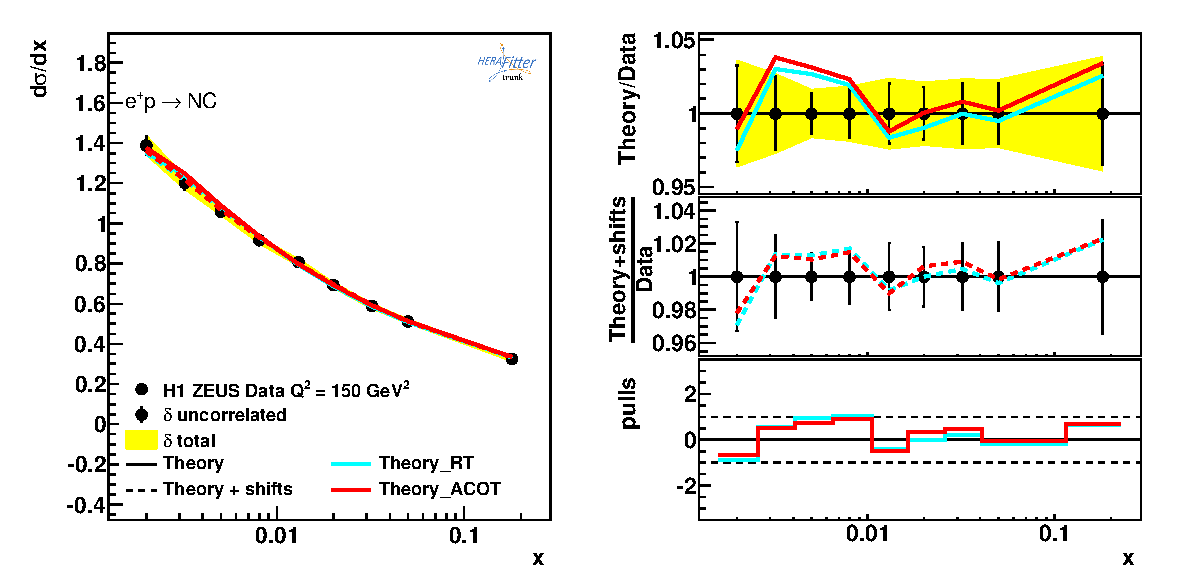
\includegraphics[width=8.6cm]{datatheory.pdf}
   \caption{An illustration of the consistency of HERA measurements~\cite{h1zeus:2009wt} and the theory predictions, 
       obtained in \fitter with the default drawing tool.} 
       %In addition, ratio plots are also provided together with the pull distribution (right panel).}    
 \label{fig:data}
\end{figure}


In \fitter there are also available cache options for fast retrieval, fast evolution kernels, and the OpenMP (Open Multi-Processing) 
interface which allows parallel applications of the GM-VFNS theory predictions in DIS. 
In addition, the \fitter references and GNU public licence are provided 
together with the main source code. 




\section{Applications of \fitter}
\label{sec:examples}
The \fitter project has successfully introduced into a wide variety
of tools to facilitate investigations of the HEP experimental data
and theoretical calculations. It provides a versatile interface
for understanding and interpreting new data and the derived PDFs.
%in the context of precision QCD theory. 
%\fitter\ has been successfully integrated in the high energy community 
%as a much needed means to provide understanding and interpretation 
%of new measurements in the context of QCD theory, a field limited by the precision of the PDFs.  
The \fitter platform not only allows the extraction of PDFs but also of theory 
parameters such as the strong coupling and heavy quark masses. The parameters and distributions are output with a
quantitative asssessment of the fit quality with fully detailed information on 
experimental and theoretical uncertainties.
The results are also output to PDF \lhapdf grids that can be used to study predictions for SM or beyond SM processes, as well as for the study of the impact of 
future collider measurements (using pseudo-data).


So far the \fitter platform has been used to produce grids 
from the QCD analyses performed at 
HERA (\cite{h1zeus:2009wt}), and and at the LHC, using 
measurements from ATLAS~\cite{atlas:strange,atlas:jets} (the first ever ATLAS PDF sets~\cite{atlas:grids}).
% to the QCD studies performed using pseudo-data to study the potential of possible future collider design such as LHeC.

New results that have been based on the \fitter platform include 
the following SM processes 
studied at the LHC:  inclusive Drell-Yan and $W$and $Z$ 
production~\cite{atlas:strange,atlas:hm,cms:strange};
inclusive jets~\cite{atlas:jets,cms:jets} production.
% and top measurements{\bf you need a reference for the top studies}
At HERA, the results of QCD analyses using \fitter are 
published for inclusive H1 measurements~\cite{h1:2012kk}
and the recent combination of charm production measurements 
in DIS~\cite{h1zeus:charm}.
The \fitter framework also provides an unique possibility to 
make impact studies for future colliders
as illustrated by the QCD studies that have been performed to 
explore the potential of the LHeC data~\cite{lhec:studies}.

A determination of the transverse momentum dependent gluon density using precision HERA
data obtained with \fitter has been reported in~\cite{Jung2014}. 

In addition, a recent study based on a set of parton distribution functions 
determined with the \fitter program using HERA data was performed~\cite{hfcorrpaper}.
It addresses the issue of correlations between uncertainties for the LO,
NLO and NNLO sets. These sets are then propagated to study uncertainties 
for ratios of cross sections calculated at different orders in QCD and  
a reduction of overall theoretical uncertainty is observed.




\section{Summary}
\label{sec:outlook}

\label{sec:summary}
\fitter is an open-source platform designed for studies of the structure of the proton.
It provides a unique and flexible framework with a wide variety of QCD tools to 
facilitate analyses of the experimental data and theoretical calculations. 
\fitter allows for direct comparisons of various theoretical approaches under the same settings,
different methodologies in treating the experimental and model uncertainties can be used for benchmarking studies.
The progress of \fitter is driven by the latest QCD advances in theoretical calculations and in the precision of experimental data.

The \fitter code, in version $1.1.0$, has sufficient options to reproduce the different theoretical choices made in MSTW, CTEQ and ABM fits. This will potentially make it a  
valuable tool for benchmarking and understanding differences between PDF fits. Such a study would however need to consider a range of further questions, such as the choices of
data sets, treatments of uncertainties, input parameter values, $\chi^2$ definitions and so forth. We look forward to studying these questions in future work.




%as required. Don't forget to give each section
%and subsection a unique label (see Sect.~\ref{sec:1}).
%\paragraph{Paragraph headings} Use paragraph headings as needed.
%\begin{equation}
%a^2+b^2=c^2
%\end{equation}



%%%%%%%%%%%%%%%%%%%%%%%%%%%%%%%%%%%%%%%%%%%%%%%%%%%%%%%%
%% For one-column wide figures use
%\begin{figure}
%% Use the relevant command to insert your figure file.
%% For example, with the graphicx package use
%  \includegraphics{example.eps}
%% figure caption is below the figure
%\caption{Please write your figure caption here}
%\label{fig:1}       % Give a unique label
%\end{figure}
%
%%%%%%%%%%%%%%%%%%%%%%%%%%%%%%%%%%%%%%%%%%%%%%%%%%%%%%%%
%% For two-column wide figures use
%\begin{figure*}
%% Use the relevant command to insert your figure file.
%% For example, with the graphicx package use
%  \includegraphics[width=0.75\textwidth]{example.eps}
%% figure caption is below the figure
%\caption{Please write your figure caption here}
%\label{fig:2}       % Give a unique label
%\end{figure*}
%
%%%%%%%%%%%%%%%%%%%%%%%%%%%%%%%%%%%%%%%%%%%%%%%%%%%%%%%%
%% For tables use
%\begin{table}
%% table caption is above the table
%\caption{Please write your table caption here}
%\label{tab:1}       % Give a unique label
%% For LaTeX tables use
%\begin{tabular}{lll}
%\hline\noalign{\smallskip}
%first & second & third  \\
%\noalign{\smallskip}\hline\noalign{\smallskip}
%number & number & number \\
%number & number & number \\
%\noalign{\smallskip}\hline
%\end{tabular}
%\end{table}

%%%%%%%%%%%%%%%%%%%%%%%%%%%%%%%%%%%%%%%%%%%%%%%%%%%%%%%%
\begin{acknowledgements}
\fitter developers team acknowledges the kind hospitality of DESY 
and funding by the Helmholtz Alliance "Physics at the Terascale" of the Helmholtz Association.
We are grateful to the DESY IT department for their support of the \fitter  developers.
Additional support was received from the BMBF-JINR cooperation program,
the Heisenberg-Landau program, the RFBR grant 12-02-91526-CERN~a, 
the Polish NSC project DEC-2011/03/B/ST2/00220 and 
a dedicated funding of the Initiative and Networking Fond of Helmholtz Association SO-072. 
We also acknowledge Nathan Hartland with Luigi Del Debbio for contributing to the 
implementation of the Bayesian Reweighting technique and
would like to thank R. Thorne for fruitful discussions.
\end{acknowledgements}



%%%%%%%%%%%%%%%%%%%%%%%%%%%%%%%%%%%%%%%%%%%%%%%%%%%%%%%%
% BibTeX users please use one of
%\bibliographystyle{spbasic}      % basic style, author-year citations
%\bibliographystyle{spmpsci}      % mathematics and physical sciences
%\bibliographystyle{spphys}       % APS-like style for physics
%\bibliography{}   % name your BibTeX data base


\bibliography{herafitter-epjc.bib}

%%%%%%%%%%%%%%%%%%%%%%%%%%%%%%%%%%%%%%%%%%%%%%%%%%%%%%%%%%%%%%%%%%
%% Non-BibTeX users please use
%\begin{thebibliography}{}
%%
%% and use \bibitem to create references. Consult the Instructions
%% for authors for reference list style.
%%
%\bibitem{RefJ}
%% Format for Journal Reference
%Author, Article title, Journal, Volume, page numbers (year)
%% Format for books
%\bibitem{RefB}
%Author, Book title, page numbers. Publisher, place (year)

%\end{thebibliography}


\end{document}
% end of file template.tex

